\documentclass[11pt]{article}
\usepackage[utf8]{inputenc}
\usepackage{amsmath,amsthm,amsfonts,amssymb,amscd}
\usepackage{multirow,booktabs}
\usepackage[italian]{babel}
\usepackage[table, dvipsnames]{xcolor}
\usepackage{fullpage}
\usepackage{lastpage}
\usepackage{enumitem}
\usepackage{glossaries}
\usepackage{fancyhdr}
\usepackage{mdframed}
\usepackage{float}
\usepackage{mathrsfs}
\usepackage{subfig}
\usepackage{tabularx}
\usepackage{wrapfig}
\usepackage{setspace}
\usepackage{calc}
\usepackage{multicol}
\usepackage{cancel}
\usepackage[retainorgcmds]{IEEEtrantools}
\usepackage[margin=3cm]{geometry}
\usepackage{amsmath}
\newlength{\tabcont}
\setlength{\parindent}{0.0in}
\setlength{\parskip}{0.05in}
\usepackage{empheq}
\usepackage{framed}
\usepackage[subfigure]{tocloft}
\usepackage[most]{tcolorbox}
\usepackage{xcolor}
\usepackage[toc,page]{appendix}
\usepackage{pgfplots}
\pgfplotsset{compat=1.16}
\usetikzlibrary{automata,arrows,positioning,calc}
\usepackage{hyperref}

\hypersetup{
  colorlinks   = true, %Colours links instead of ugly boxes
  urlcolor     = red, %Colour for external hyperlinks
  linkcolor    = blue, %Colour of internal links
  citecolor   = red %Colour of citations
}

\colorlet{shadecolor}{orange!15}
\parindent 0in
\parskip 10pt
\geometry{margin=1in, headsep=0.25in}
\theoremstyle{definition}
\newtheorem{defn}{Definizione}
\newmdtheoremenv{theo}{Teorema}
\newtheorem{reg}{Regola}
\newtheorem{exmp}{Esempio}
\newtheorem{exer}{Esercizio}
\newtheorem{note}{Nota}
 
\setlength\cftparskip{-2pt}
\setlength\cftbeforesecskip{1pt}
\setlength\cftaftertoctitleskip{2pt}
\newtcolorbox{mybox}[3][]
{
  colframe = #2!25,
  colback  = #2!10,
  coltitle = #2!20!black,  
  title    = {#3},
  #1,
  frame hidden,
}

\numberwithin{equation}{subsection}
\newcommand*{\info}[1]{\ensuremath{\log \frac{1}{p({#1})}}}
\newcommand{\sumx}{\ensuremath{\sum_{x \in X}}}
\newcommand{\sumy}{\ensuremath{\sum_{y \in Y}}}
\newcommand\numberthis{\addtocounter{equation}{1}\tag{\theequation}}

\begin{document}
\setcounter{section}{0}
\title{Appunti di Teoria dell'Informazione}

\thispagestyle{empty}

\begin{center}
{\LARGE \bf Appunti di Teoria dell'Informazione}\\
{\large \textit{Giovanni Bindi}} \\
{Universit\`a degli Studi di Firenze}
\end{center}

\tableofcontents

\newpage
\`E stato un ingegnere e matematico statunitense, \textbf{Claude Elwood Shannon} (1916 – 2001), che per primo ha
fatto diventare l’informazione qualcosa di ben definito e misurabile fornendo delle basi fondamentali per i
sistemi di comunicazioni.\\
Shannon ha lavorato nei laboratori Bell dal ’41 al ’72 e nel 1948 ha pubblicato “\href{http://www.math.harvard.edu/~ctm/home/text/others/shannon/entropy/entropy.pdf}{\emph{A Mathematical Theory of Communication}}” su The Bell System Technical Journal, una relazione tecnica che ora è alla base della Teoria dell’Informazione. \\
Oltre a definire e dare un’unità di misura all’informazione, la teoria di Shannon permette di rispondere anche a due domande fondamentali:
\begin{itemize}
    \item Quale è la massima compressione dei dati informativi senza perdita che si può ottenere.
    \item Quale è il massimo rate di trasmissione che si può avere per comunicazioni affidabili.
\end{itemize}
Gli studi di Shannon intendevano infatti migliorare l'efficienza della trasmissione dell’informazione: 

\textit{“Il problema fondamentale della comunicazione consiste nel riprodurre in un punto, esattamente o
approssimativamente, un messaggio selezionato in un altro punto.”}

L’importanza dei risultati degli studi di Shannon sta anche nel fatto che permettono di ridurre a forme
analitiche abbastanza semplici, problemi in realtà molto complessi e generali. \\
Dato un messaggio prodotto da una sorgente informativa, l’obiettivo della teoria dell’informazione è capire
come si deve rappresentare tale messaggio per ottenere una trasmissione efficiente dell’informazione in esso
contenuta su di un canale di comunicazione reale, ovvero soggetto a inevitabili limitazioni fisiche. \\
Questo obiettivo viene perseguito attraverso quattro passi fondamentali:
\begin{enumerate}
    \item \hyperref[sec:def]{Definizione e misura} dell’informazione di una sorgente.
    \item Capire, data una sorgente informativa, \textit{come} e \textit{quanto} è possibile ridurre il suo rate di trasmissione (\hyperref[sec:sorg]{\textit{Codifica di Sorgente}}).
    \item Definire cosa sia la capacità di comunicazione di un canale e sotto quali condizioni i dati provenienti da una sorgente informativa possono essere trasmessi in modo affidabile (\hyperref[sec:rdt]{\textit{Rate Distortion Theory}}).
    \item Come si può sfruttare al massimo la capacità di trasmissione di un canale rimuovendo (o rendendo trascurabili) gli effetti del canale di comunicazione (\hyperref[sec:can]{\textit{Codifica di Canale}}).
\end{enumerate}
\begin{figure}[H]
    \centering
    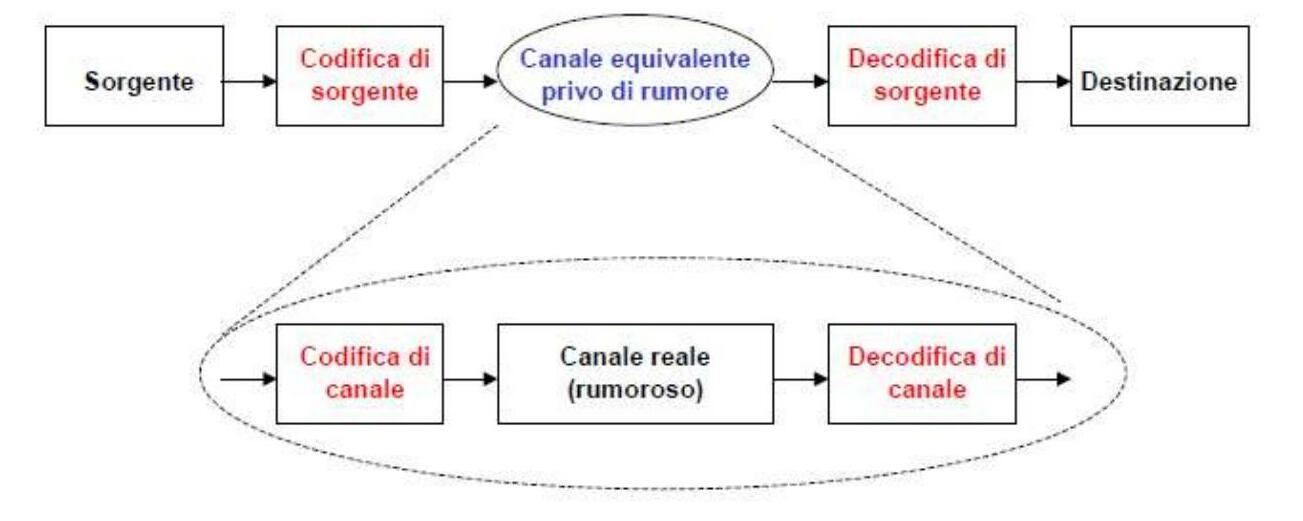
\includegraphics[scale=0.2]{img/croppedim.jpg}
    \caption{Percorso del messaggio, dalla sorgente al destinatario.}
    \label{fig:percorso}
\end{figure}
Come raffigurato in Figura \ref{fig:percorso} la codifica (sia di sorgente che di canale) si deve adattare alla sorgente e al canale in modo da avere la massima efficienza possibile nel trasferimento dell'informazione:
\begin{itemize}
    \item La \textit{codifica di sorgente} adatta la sorgente alla trasmissione su di un opportuno canale equivalente privo di rumore.
    \item La \textit{codifica di canale} permette di trasmettere l’informazione emessa dalla sorgente (opportunamente
trattata mediante la codifica di sorgente) in maniera affidabile su un canale reale caratterizzato da limitazioni fisiche.
\end{itemize}

\begin{center}
  $\ast$~$\ast$~$\ast$
\end{center}

Questi appunti sono stati elaborati principalmente sulla base del materiale pubblicato dal titolare del corso, a cui vanno tutti i crediti. I riferimenti principali oltre a questo sono stati:
\begin{enumerate}
    \item \textit{\href{https://www.wiley.com/en-it/Elements+of+Information+Theory,+2nd+Edition-p-9780471241959}{Elements of Information Theory} - Thomas M. Cover \& Joy A. Thomas.}
    \item \textit{\href{http://clem.dii.unisi.it/~vipp/files/TIC/dispense.pdf}{Lecture notes on Information Theory and Coding} - Mauro Barni \& Benedetta Tondi.}
    \item \textit{\href{http://www.inference.org.uk/mackay/itprnn/book.html}{Information Theory, Pattern Recognition, and Neural Networks} - David MacKay.}
\end{enumerate}
Chiunque volesse contribuire a questo materiale, segnalando degli errori o estendendo il contenuto, mi pu\`o contattare a \href{mailto:gio.bindi@pm.me}{gio.bindi@pm.me}.
\begin{flushright}
Novembre 2019.
\end{flushright}

\newpage
\section{Definizioni fondamentali e primi risultati} \label{sec:def}

\subsection{Sorgenti}
In generale si dice sorgente $S$ un oggetto che emette\footnote{In questi appunti spesso si user\`a lo stesso simbolo sia per la sorgente che per l'alfabeto, anche se ci sono testi in cui si fa differenza, come in \href{http://www.inference.org.uk/mackay/itprnn/book.html}{Information Theory, Inference, and Learning Algorithms}.} simboli $x$ appartenenti ad un alfabeto $X$. La sorgente è nota quando conosciamo la probabilità con cui viene emesso ciascun simbolo. Possiamo distinguere tra:
\begin{itemize}
    \item Sorgenti \textbf{discrete}, in cui l'alfabeto \`e un insieme finito.
    \item Sorgenti \textbf{continue}, in cui l'alfabeto \`e un insieme di simboli infinito numerabile.
\end{itemize}

Sappiamo, comunque, che qualsiasi sorgente continua può essere trasformata in una sorgente numerica (in
particolare digitale) grazie alle operazioni di campionamento e quantizzazione. Le sorgenti con cui abbiamo a che fare nei moderni sistemi informativi sono infatti sostanzialmente sempre sorgenti discrete. Per questo motivo la nostra attenzione sarà principalmente rivolta alle sorgenti discrete anche se poi i risultati verranno generalizzati al caso continuo perché ci sono contesti (in particolare il canale di comunicazione) in cui abbiamo a che fare con segnali/sorgenti continui. \\
I simboli emessi dalla sorgente sono delle \hyperref[sec:prob]{\textbf{variabili aleatorie}} (altrimenti \textit{non ci sarebbe informazione da
trasmettere}) e quindi ci si riferisce sempre a variabili e processi aleatori. Quando, infatti, si considera l’emissione successiva di simboli nel tempo si ha un \hyperref[sec:stoc]{\textbf{processo stocastico}}, ovvero una sequenza di variabili aleatorie indicizzate nel tempo.

Un'altra distinzione che possiamo fare nelle sorgenti dipende dal legame tra simboli successivi (emessi ad istanti successivi dalla sorgente). Se questi sono dipendenti gli uni dagli altri la sorgente si dice \textbf{con memoria}, altrimenti si dice \textbf{senza memoria} e le variabili aleatorie sono indipendenti e identicamente distribuite. \\
Le sorgenti senza memoria sono più semplici ma più rare. Un lancio di monete è una sorgente senza memoria: in questo caso basta conoscere la probabilità di ogni singolo simbolo perché la probabilità congiunta è il prodotto delle singole probabilità. Le sorgenti con memoria invece sono più complesse ma sono anche quelle che di solito si trovano in pratica, e sono caratterizzate dalle probabilità congiunte. Ad esempio un testo scritto: ci sono ovviamente dei legami tra le lettere che escono, ad esempio una $q$ è seguita da una $u$, perché devono rispettare una sintassi. 
\subsection{Informazione ed Entropia}
Prima di tutto il problema della teoria dell’informazione è definire, rappresentare matematicamente e
quantificare l’informazione che viene prodotta da una sorgente. L’informazione può essere di tipo:
\begin{itemize}
    \item \textbf{Semantico}, ovvero riguardare il significato del messaggio.
    \item \textbf{Sintattico}, ovvero riguardare i simboli che si usano e come questi sono relazionati tra loro - come \`e costruito il messaggio.
\end{itemize}
La teoria dell’informazione si occupa \textit{solo dell’aspetto \textbf{sintattico}} (o simbolico): a livello di sistema di comunicazione non ci interessa la semantica, ovvero cosa significa un dato messaggio (dal momento che incontriamo il problema della soggettività dell’informazione) ma la \textit{quantità} di informazione che questo porta.\\ 
Shannon sviluppò l’idea di definire l’informazione legata ad un evento $x$ solo in relazione
alla probabilità $p(x)$ che quell’evento avvenga, in particolare ebbe l'intuizione di imporre che il contenuto informativo dell'evento fosse tanto maggiore quanto pi\`u bassa fosse la probabilit\`a dell'evento associato. Le propriet\`a che la definizione di informazione $I(\cdot)$ deve soddisfare sono:
\begin{itemize}
    \item Deve essere una funzione (continua) della probabilit\`a: $I(x) = f(p(x))$ e deve essere $f(p(x)) \in (0,1]$ (un evento che non pu\`o avvenire non \`e di interesse). 
    \item Deve essere $I(1) = 0$, dal momento che un evento certo non porta informazione.
    \item Deve essere $p(x) \to 0^+ \implies I(x) \to \infty$, ovvero che un evento raro porti molta informazione, e quindi che la funzione $f$ sia decrescente.
\end{itemize}

Sia $S$ una sorgente (una variabile aleatoria discreta) che emette simboli su un alfabeto $X=\{x_1, x_2, \dots, x_M\}$ con una distribuzione $p(x) = Pr\{S=x\}, x\in X$.
\defn{\textit{Informazione}}: L'informazione associata al simbolo $x$ \`e definita\footnote{Il logaritmo si intende implicitamente in base 2 anche se pu\`o essere ovviamente operato un cambio di base: $\log_b p = \log_b a \log_a p$. In questo caso cambia solamente l'unit\`a con cui si misura l'informazione. Per $b=2$ si ha il $bit$, per $b=3$ il $trit$, per $b=e$ il $neper$ e cos\`i via. Si veda la Figura \ref{fig:autoinf}b per l'andamento della funzione di informazione al variare della base $b$.} come 
\begin{equation}
I(x) \coloneqq \log \frac{1}{p(x)}
\end{equation}
Se si hanno più eventi \textit{indipendenti}, essendo la probabilità congiunta degli eventi il prodotto delle probabilità, l’informazione complessiva è la somma delle singole informazioni:
\begin{equation}
I(x, y) = \log \frac{1}{p(x,y)} = \log \frac{1}{p(x)p(y)} = \log \frac{1}{p(x)} + \log \frac{1}{p(y)} = I(x) + I(y)
\end{equation}
\textit{\`E importante sottolineare come l’informazione sia solo legata alla probabilità  che un evento accada, non è in alcun modo legata alla natura dell'evento}. \\
Se consideriamo una sorgente $S$ discreta senza memoria (DMS): si ha che l'informazione media della sorgente \`e data dal valore atteso dell'informazione:

\defn{\textit{Entropia}}: L'entropia associata alla sorgente DMS \`e definita come
\begin{equation}
H(S) \coloneqq \mathbb{E}_p [I(x)] =  \sum_{x \in X} p(x) \info{x} = - \sum_{x \in X} p(x) \log p(x)
\end{equation}
e si misura in \textit{bit/simbolo}. Vedremo pi\`u avanti come l’entropia dia una misura del “costo minimo” per rappresentare un’informazione, ovvero il \textit{minimo numero medio di bit che servono per rappresentare le informazioni inviate da una sorgente}. \\
Quando si ha $p(x)=0$ si adotta la convenzione $0 \times \info{0} \coloneqq 0$ dal momento che 
\begin{equation}
\lim_{x\to0^+} x \log \frac{1}{x} = 0
\end{equation}

\begin{figure}[!tbp]
  \centering
  \subfloat{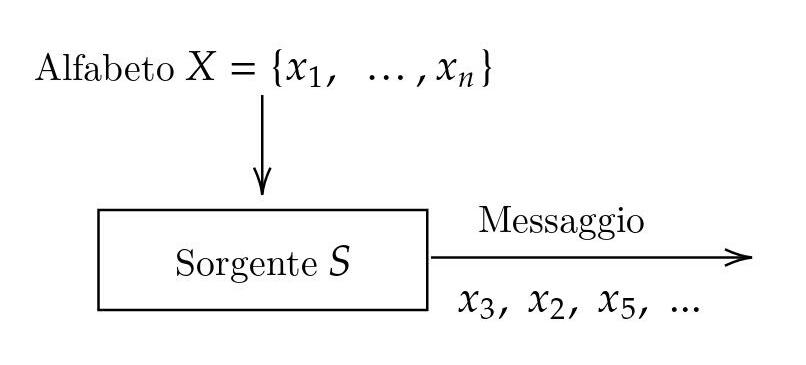
\includegraphics[width=0.5\textwidth]{img/sorgente.jpg}\label{fig:sorge}}
  \hspace{15pt}
\begin{tikzpicture}[thick,scale=0.65]
\begin{axis}[domain=-.5:20, samples=1000,grid=major,
    restrict y to domain=0:5,xlabel=$p(x)$,ylabel=$I(x)$, ylabel style={rotate=-90},]
          \addplot [color=red]    {-log2(x)};
\addplot [color=green]  {-log2(x)/log2(e)};
\addplot [color=blue] {-log2(x)/log2(10)}; 
\legend{$b=2$, $b=e$, $b=10$}
\end{axis}
\end{tikzpicture}
  \caption{Rappresentazione schematica di una sorgente e grafico della funzione di informazione.}
  \label{fig:autoinf}
\end{figure}

\begin{mybox}{green}{\textit{\textbf{Esempio 1} : \textbf{Sorgente Binaria}}}
Consideriamo una sorgente $S$ che emette due soli simboli: $X = \{x,y\}$ con probabilit\`a $p(x) = q$ e $p(y) = 1- q$. Si ha che 
\begin{equation}
H(S) = H(q) = q \log \frac{1}{q} + (1-q)\log \frac{1}{1-q}
\end{equation}
Ad esempio se $q=0.7$ si avrebbe $H(q) \approx 0.88$ $bit/simbolo$. Quand'\`e che l'entropia di una sorgente binaria \`e massima? Si vede facilmente che il massimo si ottiene in:
\begin{align*}
    &\frac{d}{dq} H(q) = \frac{d}{dq} \Big \{ -q \log q - (1-q) \log{1-q} \Big \} = \\
    &= - \Big \{ \log q + q \frac{1}{q} \log e -\log(1-q) - (1-q)\frac{1}{1-q} \log e \Big \} = \\
    &= \log{(1-q)} - \log{q} = 0 
\end{align*}
ovvero quando si ha
\[
1-q = q \implies q = \frac{1}{2}
\]
Quindi si ha che l'entropia di una sorgente binaria \`e massima quando i due simboli sono equiprobabili e vale $H(q) = 1$.

\begin{figure}[H]
    \centering
    \begin{tikzpicture}[thick,scale=0.9, every node/.style={scale=0.9}]
\begin{axis}[domain=0:1, samples=100,grid=major,
    restrict y to domain=0:1,xlabel=$q$,ylabel=$H(q)$, ylabel style={rotate=-90},]
          \addplot [color=blue]    {-x*log2(x) - (1-x)*log2(1-x)};
\end{axis}
\end{tikzpicture}
    \caption{Entropia di una sorgente binaria, al variare di $q$.}
    \label{fig:binentropy}
\end{figure}
\end{mybox}

Si hanno poi queste due propriet\`a, in cui la seconda \`e una generalizzazione di quanto appena visto per una sorgente binaria:
\begin{enumerate}
    \item $H(S) \geq 0$ dal momento che $0 \leq p(x) \leq 1 \implies \info{x} \geq 0$. 
    \item $H(S) \leq \log M$ con $H(S) = \log M \iff$ i simboli sono equiprobabili.
\end{enumerate}
Vediamo la dimostrazione per questa seconda propriet\`a: 
\begin{tcolorbox}[enhanced, breakable, frame hidden]
\textbf{Dim}: Vogliamo provare che $H(S) - \log M \leq 0$. Si ha che
\begin{align*}
&H(S) - \log M = \\
&= \sum_{x \in X} p(x) \info{x} - \log M \overset{\alpha}{=} \\
&= \sum_{x \in X} p(x) \info{x} - \sum_{x \in X} p(x) \log M = \\
&= \sum_{x \in X} p(x) \Big ( \log \frac{1}{Mp(x)} \Big ) = \\
&= \log{e} \bigg [ \sum_{x \in X} p(x) \Big ( \ln \frac{1}{Mp(x)} \Big ) \bigg ] \overset{\beta}{\leq} \\
&\leq \log{e} \bigg [ \sum_{x \in X} p(x) \Big ( \frac{1}{Mp(x)} - 1 \Big ) \bigg ] = \\
&= \log{e} \bigg [ \sum_{x \in X} \Big ( \frac{1}{M} - p(x) \Big ) \bigg ] = \\
&= \log{e} \bigg [ 1 - \sum_{x \in X} p(x) \bigg] \overset{\alpha}{=} 0 \\
\end{align*} 
Si ha poi che la disuguaglianza vale con l'uguale quando, $\forall x \in X$:
\[
\ln \frac{1}{Mp(x)} = \frac{1}{Mp(x)} -1 \iff \frac{1}{Mp(x)} = 1 \iff p(x) = \frac{1}{M}
\]
ovvero quando tutti i simboli $x$ sono equiprobabili. $\square$
\end{tcolorbox}
Dette $p,q$ due distribuzioni sullo stesso alfabeto $X$ si definisce una quantit\`a importante: 
\defn{\textit{Entropia Relativa}}: L'entropia relativa, detta anche \textit{divergenza di Kullback-Leibler} è una misura non simmetrica{\footnote{Anche se è spesso pensata come una distanza, la divergenza KL non è una vera e propria metrica - per esempio, infatti, non è simmetrica: la KL da $p$ a $q$ non è in genere la stessa KL da $q$ a $p$. Tuttavia, la sua forma infinitesimale, in particolare la sua matrice Hessiana, è un tensore metrico: \`e l'\href{https://it.wikipedia.org/wiki/Informazione_di_Fisher}{informazione metrica di Fisher}. Oltre a non essere simmetrica non pu\`o essere una distanza dal momento che non vale la disuguaglianza triangolare.}} della differenza tra due distribuzioni di probabilità. Misura infatti l'inefficienza (la perdita di informazione che si ha) nell'assumere che la distribuzione di probabilit\`a sia $q$ quando quella reale \`e $p$.
\begin{equation}
D(p\|q) \coloneqq \sum_{x \in X} p(x) \log \frac{p(x)}{q(x)}
\end{equation}
Anche per l'entropia relativa si pu\`o mostrare un'importante propriet\`a, quella della non-negativit\`a:
\begin{itemize}
    \item $D(p \| q) \geq 0$ con $D(p \| q) = 0 \iff p = q$
\end{itemize}
\begin{tcolorbox}[enhanced, breakable, frame hidden]
\textbf{Dim}: Vogliamo mostrare che $-D(p \| q) \leq 0$. Si ha:
\begin{align*}
    -D(p \| q) = \sum_{x \in X} p(x) \log \frac{q(x)}{p(x)} = \log e \sum_{x \in X} p(x) \ln \frac{q(x)}{p(x)} \overset{\beta}{\leq} \\
    \leq \log e \sum_{x \in X} p(x) \Big ( \frac{q(x)}{p(x)} - 1 \Big ) = \log e \Big ( \sum_{x \in X} q(x) - \sum_{x \in X} p(x) \Big ) = 0 \\
    \square
\end{align*}
\end{tcolorbox}
L'entropia relativa \`e importante in molti ambiti diversi della teoria dell'informazione (e non solo) ed ha una interpretazione legata alla costruzione dei codici: se  abbiamo  una  sorgente $S$ che  emette  simboli con distribuzione $p$ per rappresentarla  possiamo costruire un  codice con lunghezza  $H(p)$ bit/simbolo, se però usiamo un codice costruito per una  distribuzione $q$ c’è bisogno  in media di una lunghezza  $H(p)+D(p\|q)$ per rappresentarla. \\
Data una variabile aleatoria congiunta $(X, Y)$ con distribuzione di probabilit\`a congiunta $p(x,y)$ si definisce l'entropia congiunta delle variabili $X$ e $Y$ come
\defn{\textit{Entropia Congiunta}}: \\ Sia $x \in X = \{x_1, \dots, x_M \}$ e $y \in Y = \{y_1, \dots, y_Q \}$ una coppia di variabili aleatorie con distribuzione congiunta $p(x,y)$. Si ha che l'entropia congiunta tra $X$ e $Y$ \`e definita come:
\begin{equation}
H(X,Y) \coloneqq \sum_{x \in X} \sum_{y \in Y} p(x,y) \log \frac{1}{p(x,y)}
\end{equation}
Una quantit\`a strettamente correlata all'entropia congiunta \`e la:
\defn{\textit{Entropia Condizionata}}: L'entropia condizionata \`e definita come:
\begin{equation}
H(X|Y) = \sum_{x \in X} \sum_{y \in Y} p(x,y) \log \frac{1}{p(x|y)}
\end{equation}
Per quanto riguarda il rapporto tra entropia congiunta e condizionata si pu\`o vedere che:
\begin{equation}
H(X,Y) = H(X) + H(Y|X) = H(Y) + H(X|Y)
\end{equation}
che prende il nome di \textit{chain rule} per l'entropia.
\begin{tcolorbox}[enhanced, breakable, frame hidden]
\textbf{Dim}: Mostriamo che $H(X,Y) = H(X) + H(Y|X)$, vale l'analogo per l'altro caso.
\begin{align*}
    H(X,Y) &= \sum_{x \in X} \sum_{y \in Y} p(x,y) \log \frac{1}{p(x,y)} \overset{\gamma}{=} \sum_{x \in X} \sum_{y \in Y} p(x,y) \log \frac{1}{p(y|x)p(x)} = \\
    &= \sum_{x \in X} \sum_{y \in Y} p(x,y) \Big [ \log \frac{1}{p(x)} + \log \frac{1}{p(y|x)} \Big] = 
\end{align*}
\begin{align*}
    &= \sum_{x \in X} \sum_{y \in Y} p(x,y) \log \frac{1}{p(x)} + \sum_{x \in X} \sum_{y \in Y} p(x,y) \log \frac{1}{p(y|x)} = \\
    &\overset{\delta}{=} \sum_{x \in X} p(x) \info{x} + \sum_{x \in X} \sum_{y \in Y} p(x,y) \log \frac{1}{p(y|x)} = \\
    &= H(X) + H(Y|X) \hspace{200pt} \square
\end{align*}
\end{tcolorbox}
La chain rule per l'entropia pu\`o essere generalizzata a $m$ variabili aleatorie $X_1, X_2, \dots, X_m$:
\begin{equation}
    H(X_1, X_2, \dots, X_m) = H(X_1) + H(X_2|X_1) + H(X_3|X_1, X_2) + \dots + H(X_m|X_1, \dots, X_{m-1})
\end{equation}
ricordando che la chain rule per la probabilit\`a \`e data da:
\begin{equation}
\label{eqn:probchain}
    p(x_1, x_2, \dots, x_m) = p(x_1) \cdot p(x_2|x_1) \cdot p(x_3|x_1, x_2) \cdot \dots \cdot p(x_m|x_1, \dots, x_{m-1})
\end{equation}
Una propriet\`a importante dell'entropia condizionata \`e che, in generale, si ha
\begin{equation}
    H(X|Y) \leq H(X)
\end{equation}
ovvero che il condizionamento non pu\`o far aumentare l'entropia (\textit{information can't hurt}).
\begin{tcolorbox}[enhanced, breakable, frame hidden]
\textbf{Dim}: Mostriamo che $H(X|Y) - H(X) \leq 0$
\begin{align*}
    H(X|Y) - H(X) &= \sum_{x \in X} \sum_{y \in Y} p(x,y) \log \frac{1}{p(x|y)} - \sum_{x \in X} p(x) \info{x} \overset{\delta}{=} \\
    &= \sum_{x \in X} \sum_{y \in Y} p(x,y) \log \frac{1}{p(x|y)} - \sum_{x \in X} \sum_{y \in Y} p(x,y) \info{x} =\\
    &= \sumx \sumy p(x,y) \log \frac{p(x)}{p(x|y)} = \log e \sumx \sumy p(x,y) \ln \frac{p(x)}{p(x|y)} \overset{\beta}{\leq} \\
    &\leq \log e \sumx \sumy p(x,y) \Big [ \frac{p(x)}{p(x|y)} - 1 \Big ] = \log e \sumx \sumy p(x,y) \Big [ \frac{p(x)p(y)}{p(x,y)} - 1 \Big] = \\ 
    &= \log e \bigg [ \sumx p(x) \sumy p(y) - \sumx \sumy p(x,y) \bigg] = 0 \hspace{100pt} \square
\end{align*}
\end{tcolorbox}
Ovviamente vale anche $H(Y|X) \leq H(Y)$ per cui, per l'entropia congiunta, vale anche questa disuguaglianza:
\begin{equation}
\label{eqn:leq}
    H(X,Y) \leq H(X) + H(Y)
\end{equation}

\subsection{Informazione Mutua}
Un'altra grandezza fondamentale \`e l'informazione mutua tra due sorgenti. Questa misura in un certo senso il grado di dipendenza di due variabili aleatorie, ovvero misura \textit{quanta informazione di una variabile aleatoria \`e contenuta nell'altra}. Pu\`o essere pensata come la quantit\`a di riduzione dell'incertezza su una variabile aleatoria quando si osserva l'altra. \`E definita come
\defn{\textit{Informazione mutua:}} Date due variabili aleatorie $X, Y$ si ha che l'informazione mutua \`e definita come:
\begin{equation}
    I(X;Y) \coloneqq \sumx \sumy p(x,y) \log \frac{p(x,y)}{p(x)p(y)}
\end{equation} 
Data questa definizione si vede subito che
\begin{equation}
    I(X;Y) = D \Big ( p(x,y) \| p(x)p(y) \Big )
\end{equation}
ovvero che l'informazione mutua \`e \textit{l'entropia relativa tra la distribuzione congiunta e il prodotto delle marginali}. Da questa considerazione si ha subito una prima propriet\`a per l'informazione mutua:
\begin{equation}
    I(X;Y) \geq 0
\end{equation}
Si ha inoltre che, se le due variabili aleatorie sono indipendenti, $p(x,y) = p(x)p(y)$, si ha $I(X;Y) = 0$ ovvero non c'\`e distanza tra le due distribuzioni. Viceversa più le variabili aleatorie sono tra loro legate più l’informazione mutua cresce, difatti la differenza tra la distribuzione congiunta e il prodotto delle due aumenta. \\
Se $X$ e $Y$ sono indipendenti, allora la conoscenza di $X$ non dà alcuna informazione riguardo a $Y$ e viceversa, perciò la loro mutua informazione è zero. All'altro estremo, se $X$ e $Y$ sono identiche allora tutte le informazioni trasmesse da $X$ sono condivise con $Y$: la conoscenza di $X$ determina il valore di $Y$ e viceversa.\\
L’informazione mutua è strettamente collegata all’entropia, infatti:
\begin{equation}
    I(X;Y) = H(X) - H(X|Y) = H(Y) - H(Y|X)
\end{equation}
\begin{tcolorbox}[enhanced, breakable, frame hidden]
\textbf{Dim}: Mostriamo che $I(X;Y) = H(X) - H(X|Y)$, l'altro caso \`e equivalente.
\begin{align*}
    I(X;Y) &= \sumx \sumy p(x,y) \log \frac{p(x,y)}{p(x)p(y)} = \sumx \sumy p(x,y) \frac{p(x|y)p(y)}{p(x)p(y)} = \\
    &= \sumx \sumy p(x,y) \log \frac{p(x|y)}{p(x)} = \sumx \sumy p(x,y) \Big [ \log \frac{1}{p(x)} - \log \frac{1}{p(x|y)} \Big ] = \\
    &= \sumx \sumy p(x,y) \log \frac{1}{p(x)} - \sumx \sumy p(x,y) \log \frac{1}{p(x|y)} =\\ 
    & = \sumx p(x) \info{x} - \sumx \sumy p(x,y) \log \frac {1}{p(x|y)} = H(X) - H(X|Y) \hspace{30pt} \square
\end{align*}
\end{tcolorbox}
In sostanza quindi l’informazione mutua è una differenza tra entropie: l’entropia di una variabile aleatoria meno l’incertezza di quella variabile aleatoria una volta che ho conosciuto l'altra. Si ha inoltre che
\begin{itemize}
    \item L'informazione mutua \`e simmetrica: $I(X;Y) = I(Y;X)$.
    \item $I(X;Y) = H(X) + H(Y) - H(X,Y)$ (dalla chain rule per l'entropia).
    \item Nel caso discreto vale $I(X;X) = H(X)$ (dal fatto che $H(X|X) = 0$) per cui si ha $I(X;X) \geq I(X;Y)$, ovvero che una variabile $X$ contiene almeno tanta informazione riguardo a sé stessa di quanta ne può fornire una qualsiasi altra variabile $Y$.
\end{itemize}
\begin{figure}[!tbp]
  \centering
  \subfloat{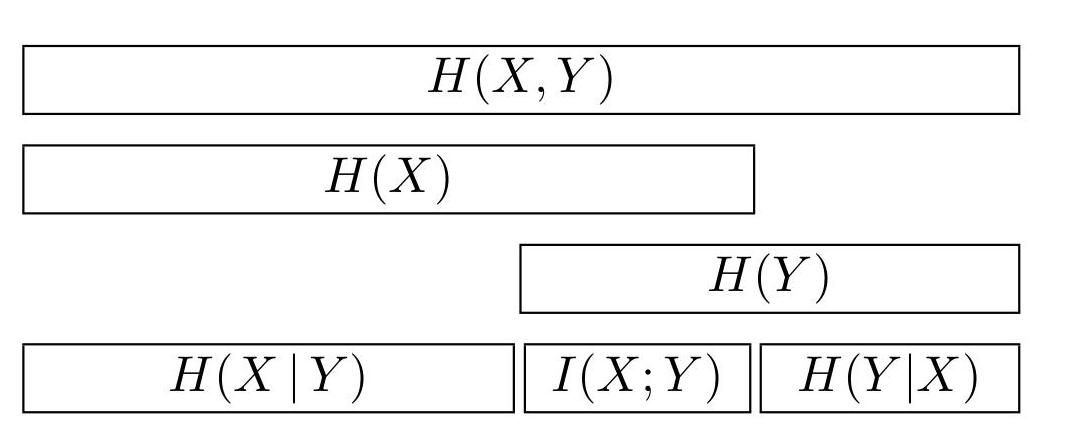
\includegraphics[width=0.4\textwidth]{img/infomut.jpg}\label{fig:f1}}
  \hspace{25pt}
  \subfloat{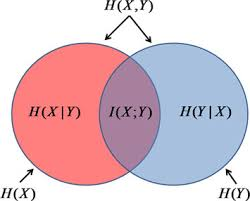
\includegraphics[scale=0.5]{img/mutinfo.jpg}\label{fig:f2}}
  \caption{Due rappresentazioni equivalenti delle relazioni tra entropia e informazione mutua.}
\end{figure}

\subsection{Estensione di una sorgente}
Siano $X_1, X_2, \dots, X_n$ un numero $n$ di variabili aleatorie identicamente distribuite ($i.d.$) (come ad esempio nella trasimissione di un messaggio in cui ogni simbolo emesso appartiene allo stesso alfabeto). L'entropia congiunta di queste $n$ variabili aleatorie rappresenta una grandezza importante:
\begin{equation}
    H(X_1, X_2, \dots, X_n) = \sum_{x_1 \in X_1} \sum_{x_2 \in X_2} \dots \sum_{x_n \in X_n} p(x_1, x_2, \dots, x_n) \log \frac{1}{p(x_1, x_2, \dots, x_n)}
\end{equation}
\defn{\textit{Estensione della sorgente:}} La quantit\`a $(X_1, X_2, \dots, X_n)$ prende il nome di estensione della sorgente e si indica con $X^n$. Dal momento che queste $n$ variabili aleatorie sono $i.d$ si ha che $H(X) = H(X_1) = H(X_2) = \dots = H(X_n)$. Nel caso in cui non si ha memoria, oveero quando queste $n$ variabili aleatorie sono anche indipendenti (sono quindi $i.i.d$) si ha che
\begin{equation}
    H(X^n) \coloneqq H(X_1, X_2, \dots, X_n) = nH(X)
\end{equation}
\begin{tcolorbox}[enhanced, breakable, frame hidden]
\textbf{Dim}:
\begin{align*}
    &H(X_1, X_2, \dots, X_n) = \sum_{x_1 \in X_1} \sum_{x_2 \in X_2} \dots \sum_{x_n \in X_n} p(x_1, x_2, \dots, x_n) \log \frac{1}{p(x_1, x_2, \dots, x_n)} = \\
    &=\sum_{x_1 \in X_1} \sum_{x_2 \in X_2} \dots \sum_{x_n \in X_n} p(x_1)p(x_2)\dots p(x_n) \log \frac{1}{p(x_1)p(x_2)\dots p(x_n)} = \\
    &=\sum_{x_1 \in X_1} \sum_{x_2 \in X_2} \dots \sum_{x_n \in X_n} p(x_1)p(x_2)\dots p(x_n) \Big [ \info{x_1} + \info{x_2} \dots + \info{x_n} \Big]
\end{align*}
Si ha quindi la somma di $n$ termini. Analizziamo il generico elemento $k$ di questa somma:
\begin{align*}
    &\sum_{x_1 \in X_1} \dots \sum_{x_k \in X_k} \dots \sum_{x_n \in X_n} p(x_1) \dots p(x_k) \dots p(x_n) \info{x_k} = \\
    &\underbrace{\sum_{x_1 \in X_1} \dots \sum_{x_n \in X_n} p(x_1) \dots p(x_n)}_{=1} \sum_{x_k \in X_k} p(x_k) \info{x_k} = H(X_k)
\end{align*}
Quindi, considerando tutti gli $n$ termini $i.i.d$ vale:
\[
H(X_1, X_2, \dots, X_n) = H(X_1) + H(X_2) = \dots + H(X_n) = n H(X) \qquad \square
\]
\end{tcolorbox}
\subsection{Entropy Rates}
Consideriamo ora sorgenti in cui l’emissione di un simbolo \textit{non è indipendente} dai simboli emessi in
precedenza dalla sorgente. Non si può più applicare quindi la definizione di entropia vista per una sorgente
DMS, perché in questo caso l’informazione media portata da un simbolo della sorgente deve tenere in
considerazione lo \textbf{stato} in cui si trova la sorgente (ovvero le relazioni del simbolo con quelli precedenti).
Una sorgente con memoria è caratterizzata da uno stato che è rappresentato dai simboli emessi in
precedenza. In questo caso vale quindi
\begin{equation}
    H(X_1, X_2, \dots, X_n) < H(X_1) + H(X_2) + \dots H(X_n) = n H(X)
\end{equation}
a causa della dipendenza dalle variabili.

Per definire l’entropia di una sorgente con memoria si deve tenere in considerazione la dipendenza tra simboli
successivi. Se volessimo definire l’informazione media portata da un simbolo potremmo distinguere due casi:
\begin{itemize}
    \item L’entropia congiunta di tutti i simboli emessi successivamente dalla sorgente e poi divisa per $n$, per avere l’informazione media per simbolo con $n \to \infty$ (asintoticamente): 
    \begin{equation}
    \lim_{n \to \infty} \frac{H(X_1, X_2, \dots, X_n)}{n}
    \end{equation}
    \item L’informazione che viene portata da un simbolo, condizionata a tutti i simboli precedentemente
emessi, quando $n \to \infty$, ovvero tenendo conto di infinite relazioni con i simboli precedenti
    \begin{equation}
    \lim_{n \to \infty} \frac{H(X_n|X_1, \dots, X_{n-1})}{n}
    \end{equation}
\end{itemize}
Questi due limiti prendono il nome di \textbf{entropy rates}.

\`E possibile dimostrare che nel caso di processi stocastici stazionari questi due limiti esistono e coincidono ma, in generale, per il limite di $n \to \infty$, calcolare le probabilit\`a condizionate diventa impossibile. Solo in alcuni casi risulta fattibile e noi in particolare noi analizzeremo il caso delle sorgenti di Markov.

\subsection{Sorgenti di Markov}
\defn{\textit{Sorgente di Markov di ordine $k$:}} Una sorgente di Markov di ordine $k$ \`e una sorgente in cui l'emissione di un simbolo ad un certo istante di tempo dipende dai $k$ simboli emessi in precedenza.

In generale si definisce processo di Markov (o anche \textit{catena di Markov}), un processo stocastico in cui la probabilità di transizione che determina il passaggio a uno stato di sistema dipende solo dallo stato del sistema immediatamente precedente (proprietà di Markov) e non da come si è giunti a questo stato.

Nel caso particolare di una sorgente di Markov di ordine $1$ l'insieme degli stati coincide con l'insieme dei simboli e la distribuzione di probabilit\`a degli stati equivale alla distribuzione di probabilit\`a dei simboli. In una sorgente di ordine $k$ la probabilit\`a di emettere il simbolo $x_i$ \`e condizionata dallo stato precedente, formato dai $\{ x_{i-1}, \dots, x_{i-k} \}$ simboli. Se supponiamo di conoscere lo stato allora abbiamo che l'informazione del simbolo $x_i$ \`e data da
\begin{equation}
    I(x_i|x_{i-1}, \dots, x_{i-k}) = \log \frac{1}{p(x_i|x_{i-1}, \dots, x_{i-k})}
\end{equation}
da cui abbiamo che l'informazione media per simbolo della sorgente quando si trova in quello stato \`e
\begin{equation}
    H(X|x_{i-1}, \dots, x_{i-k}) = \sum_{x_i \in X} p(x_i|x_{i-1}, \dots, x_{i-k}) \log \frac{1}{p(x_i|x_{i-1}, \dots, x_{i-k})}
\end{equation}
Per cui per ottenere l'entropia della sorgente dobbiamo mediare su tutti i possibili stati. Chiamiamo $\sigma_k$ l'insieme dei simboli dello stato $\sigma_k = \{ x_{i-1}, \dots, x_{i-k}\} $: si ha che questo elemento appartiene all'estensione $k$-esima della sorgente $\sigma_k \in X^k$ per cui
\begin{align*}
    H(X) &= \sum_{\sigma_k \in X^k} p(\sigma_k) \sum_{x_i \in X} p(x_i|\sigma_k) \log \frac{1}{(x_i|\sigma_k)} = \\
    &= \numberthis \label{eqn:markovsource} \sum_{\sigma_{k+1} \in X^{k+1}} p(\sigma_{k+1}) \log \frac{1}{p(x_i|\sigma_k)}
\end{align*}
dove $\sigma_{k+1} = \{ x_i, x_{i-1}, \dots, x_{i-k} \}$. Se la sorgente fosse senza memoria ($k=0$) si otterrebbe la definizione usuale di entropia ($\sigma_1 = \{x_i\}$), se fosse di ordine $k=1$ si avrebbe
\begin{equation}
\label{eqn:markov}
    H(X) = \sum_{ \{x_i, x_{i-1}\} \in X^2} p(x_i, x_{i-1}) \log \frac{1}{p(x_i | x_{i-1})}
\end{equation}
\begin{mybox}[breakable]{green}{\textit{\textbf{Esempio 2} : \textbf{Sorgente di Markov di ordine 2}}}
Consideriamo una sorgente di Markov di ordine $k=2$ sull'alfabeto binario $X=\{0,1\}$. Seguendo la notazione assumiamo che le probabilit\`a condizionali dei simboli siano:
\begin{equation*}
\begin{cases}
    p(0|00) = p(1|11) = 0.8 \\
    p(1|00) = p(0|11) = 0.2 \\
    p(0|01) = p(0|10) = p(1|01) = p(1|10) = 0.5
\end{cases}
\end{equation*}
Ovvero che, ad esempio, $p(x_i=0|x_{i-1}=0, x_{i-2}=0) = 0.8$. Dal momento che abbiamo una sorgente di ordine $2$ su un alfabeto binario si hanno $4$ stati: $\{00, 01, 10, 11\}$. Il diagramma a stati di questa sorgente \`e dato da:
\begin{center}
\begin{tikzpicture}[->, >=stealth', auto, semithick, node distance=3cm]
\tikzstyle{every state}=[fill=white,draw=black,thick,text=black,scale=1]
\node[state]    (A)                     {$01$};
\node[state]    (B)[above right of=A]   {$00$};
\node[state]    (C)[below right of=A]   {$11$};
\node[state]    (D)[below right of=B]   {$10$};
\path
(A) edge[bend left,below]      node{$0.5$}      (D)
    edge[bend right, red]    node{$0.5$}      (C)
(B) edge[bend right, red]    node{$0.2$}         (A)
    edge[loop above]    node{$0.8$}         (B)
(C) edge[loop below, red]    node{$0.8$}         (C)
    edge[bend right]     node{$0.2$}         (D)
(D) edge[bend right,right]    node{$0.5$}      (B)
    edge[bend left,above, red]     node{$0.5$}         (A);
\end{tikzpicture}
\label{fig:markov2}
\end{center}
in cui in \textcolor{red}{rosso} sono etichettate le transizioni con $1$ e in nero quelle con $0$. Il diagramma pu\`o anche essere equivalentemente scritto attraverso la matrice di transizione $P$
\begin{equation*}
    P = \begin{bmatrix}
    0.8 & 0.2 & 0 & 0 \\
    0 & 0 & 0.5 & 0.5 \\
    0.5 & 0.5 & 0 & 0 \\
    0 & 0 & 0.2 & 0.8
    \end{bmatrix}
\end{equation*}
da cui si pu\`o ricavare la distribuzione stazionaria $\pi$ come $\pi P = \pi$, ottenendo
\begin{equation*}
    \pi = \begin{bmatrix} \frac{5}{14} & \frac{2}{14} & \frac{2}{14} & \frac{5}{14} \end{bmatrix}
\end{equation*}
ovvero che
\begin{equation*}
    \begin{cases}
        p(00) = p(11) = \frac{5}{14} \\
        p(01) = p(10) = \frac{2}{14}
    \end{cases}
\end{equation*}
Infine possiamo scrivere la tabella delle probabilit\`a della sorgente
\begin{table}[H]
    \centering
    \begin{tabular}{cccc}
    \toprule
    $x_{i-1},x_{i-2},x_i$ & $p(x_i|x_{i-1},x_{i-2})$ & $p(x_{i-1},x_{i-2})$ & $p(x_{i-1},x_{i-2},x_i)$ \\
    \midrule
    $0\hspace{16pt}0\hspace{18pt}0$ & $0.8$ & $5/14$ & $4/14$ \\
    $0\hspace{16pt}0\hspace{18pt}1$ & $0.2$ & $5/14$ & $1/14$ \\
    $0\hspace{16pt}1\hspace{18pt}0$ & $0.5$ & $2/14$ & $1/14$ \\
    $0\hspace{16pt}1\hspace{18pt}1$ & $0.5$ & $2/14$ & $1/14$ \\
    $1\hspace{16pt}0\hspace{18pt}0$ & $0.5$ & $2/14$ & $1/14$ \\
    $1\hspace{16pt}0\hspace{18pt}1$ & $0.5$ & $2/14$ & $1/14$ \\
    $1\hspace{16pt}1\hspace{18pt}0$ & $0.2$ & $5/14$ & $1/14$ \\
    $1\hspace{16pt}1\hspace{18pt}1$ & $0.8$ & $5/14$ & $4/14$ \\
    \bottomrule
    \end{tabular}
\end{table}
da cui calcolare l'entropia, seguendo \ref{eqn:markovsource}, come
\begin{align*}
    H(X) &= \sum_{X^3} p(x_i, x_{i-1}, x_{i-2}) \log \frac{1}{p(x_i|x_{i-1},x_{i-2})} = \\
    &= 2 \times \frac{4}{14} \log \frac{1}{0.8} + 2 \times \frac{1}{14}\log \frac{1}{0.2} + 4 \times \frac{1}{14} \log \frac{1}{0.5} \approx 0.80 \quad bit/simbolo
\end{align*}
\end{mybox}
\subsubsection{Sorgente estesa di una sorgente di Markov}
Anche per le sorgenti con memoria si possono definire le sorgenti estese $X^n$, ovvero che emettono $n$ simboli consecutivi, con la differenza che questi simboli hanno delle relazioni di dipendenza con i simboli precedenti. Il messaggio che la sorgente emette \`e $\sigma = \{x_1, \dots, x_n \}$ e, essendo una sorgente con generica memoria $k$ si ha che per caratterizzare l'informazione media dobbiamo andare a considerare le probabilit\`a condizionate
\begin{equation*}
    p(x_1, \dots, x_n | x_{n-1}, \dots, x_{n-k})
\end{equation*}
Inoltre se $k$ \`e la memoria della sorgente di Markov e $n$ \`e l'estensione del messaggio si ha che 
\begin{equation}
    \mu \coloneqq \bigg \lceil \frac{k}{n} \bigg \rceil
\end{equation}
\textbf{\`e la memoria della sorgente estesa} $X^n$ (si ha quindi che se $k\leq n$ vale sempre $\mu=1$). Anche per le sorgenti con memoria di Markov vale la stessa relazione per quelle senza memoria, ovvero 
\begin{equation}
H(X^n) = n H(X)
\end{equation}
\begin{tcolorbox}[enhanced, breakable, frame hidden]
\textbf{Dim}: Dimostriamolo per una sorgente di ordine $k=1$ e per la sua $n$-esima estensione $X^n$. Essendo $n\geq k$ allora anche $X^n$ ha memoria $\mu = 1$. \\
Chiamiamo $\sigma_n$ il messaggio $\sigma_n = \{x_1, \dots, x_n \}$ e $\sigma_n^m$ il messaggio precedente, ovvero la sua memoria $\sigma_n^m = \{x_{1}^m, \dots, x_{n}^m\} = x_{n}^m$ dal momento che la sorgente \`e di ordine $1$. Vale quindi
\begin{equation*}
    H(X^n) = \sum_{\sigma_n \in X^n} \sum_{x_{n}^m \in X} p(\sigma_n, x_{n}^m) \log \frac{1}{p(\sigma_n|x_{n}^m)}
\end{equation*}
Inoltre $p(\sigma_n| x_n^m) = p(x_1, \dots, x_n| x_n^m) = p(x_1|x_n^m) p(x_2|x_1) \dots p(x_n|x_{n-1})$ per la propriet\`a di Markov per cui vale
\begin{align*}
    H(X^n) &= \sum_{\sigma_n \in X^n} \sum_{x_{n}^m \in X} p(\sigma_n, x_{n}^m) \log \frac{1}{p(x_1|x_n^m) p(x_2|x_1) \dots p(x_n|x_{n-1})} = \\
    &= \sum_{\sigma_n \in X^n} \sum_{x_{n}^m \in X} p(\sigma_n, x_{n}^m) \bigg [ \log \frac{1}{p(x_1|x_n^m)} + \dots \log \frac{1}{p(x_n|x_{n-1})} \bigg ]
\end{align*}
che \`e la somma di $n$ termini tutti della stessa forma. Vediamo il primo:
\end{tcolorbox}
\begin{tcolorbox}[enhanced, breakable, frame hidden]
\begin{align*}
    &\sum_{\sigma_n \in X^n} \sum_{x_{n}^m \in X} p(\sigma_n, x_{n}^m) \log \frac{1}{p(x_1|x_n^m)} = \sum_{\{x_1, \dots, x_n\} \in X^{n}} \sum_{x_{n}^m \in X} p(x_1, \dots, x_n, x_{n}^m) \log \frac{1}{p(x_1|x_n^m)} = \\
    &= \Bigg [ \sum_{x_1 \in X} \sum_{x_n^m \in X} p(x_1, x_n^m) \log \frac{1}{p(x_1|x_n^m)} \Bigg ] \Bigg [ \sum_{\{x_2, \dots, x_n\} \in X^{n-1}} \sum_{x_n^m \in X} p(x_2, \dots, x_n^m) \Bigg ] = \\
    &=\sum_{x_1 \in X} \sum_{x_n^m \in X} p(x_1, x_n^m) \log \frac{1}{p(x_1|x_n^m)} = H(X)
\end{align*}
dove l'ultima uguaglianza vale perch\`e \`e la definizione di entropia di una sorgente di Markov di ordine $1$ (anche se in una notazione differente, si veda \ref{eqn:markov}). Da questa considerazione si ha
\begin{equation*}
    H(X^n) = nH(X)
\end{equation*}
$\square$
\end{tcolorbox}
\subsubsection{Sorgente aggiunta di una sorgente di Markov}
Sia, come prima, $X = \{x_1, \dots, x_M\}$ l'alfabeto di una sorgente di Markov di ordine $k$ e siano $p(x_1), \dots, p(x_M)$ le probabilit\`a (incondizionate) di emissione dei rispettivi simboli. La \textbf{sorgente aggiunta} di $X$, indicata con $\bar{X}$ \`e una sorgente \textit{senza memoria} con lo stesso alfabeto di $X$. Si ha che vale sempre
\begin{equation}
\label{eqn:adjoint}
    H(X) \leq H(\bar{X})
\end{equation}
ovvero che \textit{i legami tra i simboli riducono l'entropia della sorgente}.
\begin{tcolorbox}[enhanced, breakable, frame hidden]
\textbf{Dim}: Si dimostra nel caso di memoria $k=1$, sfruttando la propriet\`a di positivit\`a dell'entropia relativa: $-D(\cdot || \cdot) \leq 0$. Detti $x_i, x_{i-1} \in X$ due simboli emessi dalla sorgente di Markov si ha
\begin{align*}
    &-D(p(x_i,x_{i-1})||p(x_i)p(x_{i-1})) =\sum_{x_i} \sum_{x_{i-1}} p(x_i,x_{i-1}) \log \frac{p(x_i)p(x_{i-1})}{p(x_i,x_{i-1})} = \\
    &= \sum_{x_i} \sum_{x_{i-1}} p(x_i,x_{i-1}) \log \frac{p(x_i)p(x_{i-1})}{p(x_i|x_{i-1})p(x_{i-1})} = \sum_{x_i} \sum_{x_{i-1}} p(x_i,x_{i-1}) \log \frac{p(x_i)}{p(x_i|x_{i-1})} = \\
    &= \sum_{x_i} \sum_{x_{i-1}} p(x_i,x_{i-1}) \Big [ \log p(x_i) + \log \frac{1}{p(x_i|x_{i-1})}  \Big ] = \\
    &=\sum_{x_i} p(x_i) \log p(x_i) + \sum_{x_i} \sum_{x_{i-1}} p(x_i,x_{i-1}) \log \frac{1}{p(x_i|x_{i-1})} = \\ %\end{align*}
    %\end{tcolorbox}
    %\begin{tcolorbox}[enhanced, breakable, frame hidden]
    %\begin{align*}
    &= -\sum_{x_i} p(x_i) \info{x_i} + \sum_{x_i} \sum_{x_{i-1}} p(x_i,x_{i-1}) \log \frac{1}{p(x_i|x_{i-1})} = \\
    &= -H(\bar{X}) + H(X) \leq 0
\end{align*}
Dove l'ultima uguaglianza vale perch\`e il termine 
\begin{equation*}
    \sumx p(x) \info{x} = H(\bar{X})
\end{equation*}
corrisponde proprio all'entropia della sorgente di Markov nel caso incondizionato (senza memoria) e l'altro termine per definizione (\ref{eqn:markov}) corrisponde all'entropia di una sorgente di Markov di ordine $1$.\\
$\square$
\end{tcolorbox}
Seguendo l'\hyperref[fig:markov2]{esempio 2} appena svolto si avrebbe quindi che, calcolando le marginali,
\begin{equation*}
    \begin{cases}
        p(x_i=0) = 4/14 + 1/14 + 1/14 + 1/14 = 7/14 = 1/2 \\
        p(x_i=1) = 1/14 + 1/14 + 1/14 + 4/14 = 7/14 = 1/2
    \end{cases} \implies H(\bar{X}) = 1 \quad bit
\end{equation*}
che in effetti risulta maggiore dell'entropia precedentemente calcolata $H(\bar{X}) = 1 > 0.80 = H(X)$.
\subsubsection{Sorgente aggiunta di una sorgente estesa di Markov}
Si considera ora $\overline{X^n}$: la sorgente estesa dell'estensione $n$-esima di una sorgente di Markov di ordine $k=1$. Questa sorgente emette messaggi $\sigma_n = \{x_1, \dots, x_n \} \in X^n$ con probabilit\`a indipendenti dal passato, senza memoria. L'entropia di questa sorgente \`e definita come
\begin{equation}
    H(\overline{X^n}) = \sum_{\sigma_n \in X^n} p(\sigma_n) \log \frac{1}{p(\sigma_n)} = \sum_{X^n} p(x_1, \dots, x_n) \log \frac{1}{p(x_1, \dots, x_n)}
\end{equation}
e vale
\begin{equation}
\label{eqn:adjmarko}
    H(\overline{X^n}) = H(\bar{X}) + (n-1)H(X) = nH(X) + [H(\bar{X}) - H(X)]
\end{equation}
\begin{tcolorbox}[enhanced, breakable, frame hidden]
\textbf{Dim}: Dal Teorema di Bayes si ha che
\begin{equation*}
    p(x_1, \dots, x_n) = p(x_n|x_1, \dots, x_{n-1}) p(x_{n-1}|x_1, \dots, x_{n-2}) \dots p(x_2|x_1) p(x_1)
\end{equation*}
ed essendo $X$ una sorgente del primo ordine vale
\begin{equation*}
    p(x_1, \dots, x_n) = p(x_n|x_{n-1}) p(x_{n-1}|x_{n-2}) \dots p(x_2|x_1) p(x_1)
\end{equation*}
allora
\begin{align*}
    &H(\overline{X^n}) = \sum_{X^n} p(x_1, \dots, x_n) \log \frac{1}{p(x_1, \dots, x_n)} = \\
    &= \sum_{X^n} p(x_1, \dots, x_n) \log \frac {1}{p(x_1)p(x_2|x_1) p(x_3|x_2) \dots p(x_n|x_{n-1})} = \\
    &=\sum_{X^n} p(x_1, \dots, x_n) \Big [\log \frac {1}{p(x_2|x_1)} + \dots + \log \frac{1}{p(x_1)} \Big ] = 
    \\ 
    &=\sum_{X^n} p(x_1, \dots, x_n) \Big [\log \frac {1}{p(x_2|x_1)} + \dots + \log \frac{1}{p(x_n|x_{n-1})} \Big ] + \sum_{X^n} p(x_1, \dots, x_n) \log \frac{1}{p(x_1)} =
    \end{align*}
    \end{tcolorbox}
    \begin{tcolorbox}[enhanced, breakable, frame hidden]
    \begin{align*}
    &=\sum_{x_1, x_2} p(x_1,x_2) \log \frac{1}{p(x_2|x_1)} + \dots + \sum_{x_n,x_{n-1}} p(x_n,x_{n-1}) \log \frac{1}{p(x_n|x_{n-1})} + \sum_{x_1} p(x_1) \log \frac{1}{p(x_1)}
\end{align*}
in cui tutti i primi $(n-1)$ termini equivalgono all'entropia della sorgente $X$ di ordine $1$ con memoria mentre l'ultimo termine equivale all'entropia della sorgente $\bar{X}$ senza memoria:
\begin{equation*}
    H(\overline{X^n}) = \underbrace{H(X) + \dots + H(X)}_{n-1} + H(\bar{X}) = (n-1)H(X) + H(\bar{X}) \qquad \square
\end{equation*}
\end{tcolorbox}
In generale si pu\`o dimostrare che per sorgenti di ordine $k$ qualsiasi, detto $\epsilon_k > 0$ una costante che, se $n>k$, dipende unicamente dalla statistica della sorgente, si ha
\begin{equation}
    H(\overline{X^n}) = nH(X) + \epsilon_k
\end{equation}
per cui
\begin{equation}
    \frac{H(\overline{X^n})}{n} = H(X) + \frac{\epsilon_k}{n}
\end{equation}
che, all'aumentare della lunghezza del messaggio $n$, mostra come i \textit{\textbf{vincoli di memoria perdano peso}}
\begin{equation}
    \lim_{n \to \infty} \frac{H(\overline{X^n})}{n} = H(X)
\end{equation}
\begin{mybox}{red}{}
\textbf{Nota bene}: Si noti come l'aggiunta dell'estensione non sia equivalente all'estensione dell'aggiunta
\begin{equation}
    H(\bar{X}^n) \neq H(\overline{X^n})
\end{equation}
dal momento che $\bar{X}$ \`e una sorgente senza memoria si ha $H(\bar{X}^n) = n H(\bar{X})$ mentre dalla \ref{eqn:adjoint} si ha
\begin{equation}
    H(\overline{X^n}) \geq H(X^n) = nH(X)
\end{equation}
\end{mybox}
Riprendendo l'\hyperref[fig:markov2]{esempio 2}, in cui si \`e calcolato $H(X) = 0.80, H(\bar{X}) = 1$ $bit$, possiamo calcolare ora $H(X^2) = 2H(X) = 1.6$ $bit$ e
\begin{equation*}
    H(\overline{X^2}) = - 2 \times \frac{5}{14} \log \frac{5}{14} - 2 \times \frac{2}{14}\log \frac{2}{14} \approx 1.86 \hspace{4pt} bit
\end{equation*}
mentre $H(\bar{X}^2)$ pu\`o essere calcolato prendendo la sorgente senza memoria $\bar{X}$ e ricavando la congiunta come $p(x_i,x_{i-1})=p(x_i)p(x_{i-1})$ da cui
\begin{equation*}
    H(\bar{X}^2) = - 4 \times \frac{1}{4} \log \frac{1}{4} = 2 \hspace{4pt} bit = 2 H(\bar{X})
\end{equation*}
Si pu\`o poi calcolare $H(\overline{X^3})$ come
\begin{equation*}
    H(\overline{X^3}) = -2 \times \frac{4}{14} \log \frac{4}{14} - 6 \times \frac{1}{14} \log \frac{1}{14} \approx 2.66 \hspace{4pt} bit
\end{equation*}
Dalle propriet\`a delle catene di Markov si pu\`o poi ottenere $H(\overline{X^4}) \approx 3.47$ $bit$ calcolando $P^2 = PP$ e, consequentemente, la distribuzione congiunta con il Teorema di Bayes. Si vede quindi che la successione
\begin{equation*}
    \bigg \{H(\bar{X}), \frac{H(\overline{X^2})}{2}, \frac{H(\overline{X^3})}{3}, \frac{H(\overline{X^4})}{4} \bigg \} = \{ 1, 0.93, 0.89, 0.87 \}
\end{equation*}
gi\`a per $n=4$ si st\`a avvicinando a $H(X)$. 
\subsection{Sorgenti continue}
Sia $X$ una sorgente continua con pdf (probability density funcion) $f_X(x)$.
\defn{\textit{Entropia differenziale:}} Si definisce l'entropia differenziale di $X$ come
\begin{equation}
    h(x) = - \int_{-\infty}^\infty f_X(x) \log f_X(x) dx
\end{equation}
\textit{se tale integrale esiste}. Se l'entropia nel caso di una sorgente discreta \`e una quantit\`a sempre non-negativa nel caso di una sorgente continua questo non \`e pi\`u vero, si ha infatti che $h(x) \in \mathbb{R}$.

\begin{mybox}{green}{\textit{\textbf{Esempio 1} : \textbf{Sorgente uniforme }}}
Sia X una sorgente scalare con pdf uniforme nell'intervallo $[a,b]: f(x) \sim \mathcal{U}([a,b])$ 
\begin{equation*}
    f_X(x) = \begin{cases}
    \frac{1}{b-a} & x \in [a,b]\\
    0 & \text{altrimenti}
    \end{cases}
\end{equation*}
allora
\begin{equation*}
    h(x) = \frac{1}{b-a} \log(b-a) \int_{a}^b dx = \log(b-a)
\end{equation*}
da cui si vede che, quando $b-a < 1 \implies h(x)<0$
\end{mybox}

\begin{mybox}[breakable]{green}{\textit{\textbf{Esempio 2} : \textbf{Sorgente Gaussiana }}}
Sia $X$ una sorgente Gaussiana scalare con media nulla e varianza $\sigma^2$:
\begin{equation*}
    f_X(x) \sim \mathcal{N}(\sigma^2) =  \frac{1}{\sqrt{2 \pi \sigma^2}} e^{-\frac{x^2}{2\sigma^2}}
\end{equation*}
allora
\begin{align*}
    h(x) &= -\int_{-\infty}^{\infty} f_X(x) \log \frac{1}{\sqrt{2 \pi \sigma^2}} e^{-\frac{x^2}{2\sigma^2}}dx = \\
    &= -\int_{-\infty}^{\infty} f_X(x) \Big ( \log \frac{1}{\sqrt{2 \pi \sigma^2}} + \log e^{-\frac{x^2}{2\sigma^2}} \Big )dx = \\
    &= - \Big [ \log \frac{1}{\sqrt{2 \pi \sigma^2}} \underbrace{\int_{-\infty}^{\infty}f_X(x) dx}_{= 1}  - \frac{\log e}{2\sigma^2} \underbrace{\int_{-\infty}^{\infty} f_X(x) x^ 2 dx}_{= \sigma^2} \Big ] = \\
    &= - \log \frac{1}{\sqrt{2 \pi \sigma^2}} + \frac{1}{2} \log e = \frac{1}{2} \log 2 \pi \sigma^2 + \frac{1}{2} \log e = \\
    &= \frac{1}{2} \log 2\pi \sigma^2 e
\end{align*}
\end{mybox}

Si pu\`o dimostrare che, data una sorgente X con pdf $f_X(x)$ e varianza $\sigma^2$, la sua entropia differenziale $h(x)$ \`e limitata superiormente dall'entropia differenziale di una sorgente con pdf gaussiana con la stessa varianza $\sigma^2$. In altre parole:
\begin{equation}
    h(x) = - \int_{-\infty}^\infty f_X(x) \log f_X(x) dx \leq \frac{1}{2} \log 2\pi \sigma^2 e
\end{equation}
\begin{tcolorbox}[enhanced, breakable, frame hidden]
\textbf{Dim}: La dimostrazione si basa sull'uso della propriet\`a di non-negativit\`a dell'entropia relativa, nella sua versione differenziale:
\begin{equation}
    D(f_X(x) || g_X(x)) \coloneqq \int_{-\infty}^{\infty} f_X(x) \log \frac{f_X(x)}{g_X(x)} dx \geq 0
\end{equation}
Se prendiamo $g_X(x) \sim \mathcal{N}(\sigma^2) = \frac{1}{\sqrt{2 \pi \sigma^2}} e^{-\frac{x^2}{2\sigma^2}}$ si ha
\begin{align*}
-D(f_X(x) || g_X(x)) &= \int_{-\infty}^{\infty} f_X(x) \log \frac{g_X(x)}{f_X(x)} dx = \\
&= \int_{-\infty}^{\infty} f_X(x) \log g_X(x) dx - \overbrace{\int_{-\infty}^{\infty} f_X(x) \log f_X(x) dx}^{=-h(x)} = \\
&= h(x) + \int_{-\infty}^{\infty} f_X(x) \log \frac{1}{\sqrt{2 \pi \sigma^2}} e^{-\frac{x^2}{2\sigma^2}} dx = 
\\
&= h(x) + \int_{-\infty}^{\infty} f_X(x) \log \frac{1}{\sqrt{2 \pi \sigma^2}} dx + \int_{-\infty}^{\infty} f_X(x) \log e^{-\frac{x^2}{2\sigma^2}} dx = \\
&= h(x) + \log \frac{1}{\sqrt{2 \pi \sigma^2}} \int_{-\infty}^{\infty} f_X(x) dx - \frac{\log e}{2\sigma^2} \int_{-\infty}^{\infty} f_X(x) x^2 dx = \\ 
&= h(x) + \log \frac{1}{\sqrt{2 \pi \sigma^2}} - \frac{1}{2} \log e = \\
&= h(x) - \frac{1}{2} \log 2\pi \sigma^2 e \leq 0 \hspace{150pt} \square
\end{align*}
\end{tcolorbox}
Si ha quindi che \textit{a parit\`a di varianza le sorgenti gaussiane generano la massima informazione media}.

\newpage
\section{Compressione di Sorgente} \label{sec:sorg}
Il nostro obiettivo \`e quello di  associare  ad  ogni  simbolo informativo una sequenza di codice (di solito una sequenza binaria). Nel fare questo consideriamo sempre  una sorgente discreta di informazione, ovvero un  qualsiasi  elemento  del sistema  in  grado  di  produrre  una  successione  di  simboli  informativi ed  un canale ideale,  totalmente  affidabile, che quindi non altera l’informazione trasmessa (a ciascun simbolo inviato corrisponderà esattamente lo stesso simbolo ricevuto).
Di conseguenza l’operazione di decodifica ricostruirà esattamente i simboli della sorgente discreta originaria.
Esistono due tipi di codifiche di sorgente:
\begin{itemize}
    \item \textbf{Codifica lossy} (con perdita): si  applica  soprattutto  a  sorgenti  audio  e  video,  si  sfruttano fenomeni percettivi per    ridurre    la    quantità    di    bit    da    trasmettere. La cascata    dei processi di compressione/decompressione  porta  in  uscita  ad  un  flusso  digitale  diverso  da  quello in  ingresso. Tuttavia, si fa in modo che la perdita sia tollerabile (o addirittura irrilevante) per l’utente finale. La  compressione con perdite ha il vantaggio che può ottenere tassi di compressione molto più elevati rispetto a quella senza perdite.
    \item \textbf{Codifica lossless} (senza perdita): si  applica  \textit{solo  a  sorgenti  discrete} e  lo  scopo  della  codifica  di sorgente  è  quello  di  permettere  la  ricostruzione \textit{integrale} di  quanto  trasmesso,  che  dunque  viene detto senza perdita di informazione. La cascata dei processi di compressione/decompressione porta esattamente allo stesso flusso digitale che si ha in ingresso. 
\end{itemize}
Noi ci occuperemo della codifica lossless.
\subsection{Tipi di codice}
Un codice è una mappatura di una sequenza di simboli di una sorgente $S$ con alfabeto $X = \{x_1, \dots, x_n\}$ in una sequenza di simboli appartenenti  ad  un  altro  alfabeto $B = \{b_1, \dots, b_m\}$ di qualsiasi lunghezza.
\defn{\textit{Codice:}} Un codice \`e una funzione $C(\cdot)$ che associa ad ogni simbolo della sorgente una stringa di elementi appartenenti ad un alfabeto $B$:
\begin{equation}
    C: X \to B^*
\end{equation}
Dove $B^*$ rappresenta l'insieme di tutte le stringhe sull'alfabeto $B$. Dato un simbolo $x \in X$ la parola di codice (\textit{codeword}) associata si denota con $C(x)$.

Ovviamente non tutti i codici vanno bene, ce ne sono alcuni che sono preferibili, ed in particolare ciò che ci interessa di un codice è:
\begin{itemize}
    \item La \textbf{non ambiguit\`a}: ovvero la possibilità del ricevitore di ricostruire la successione di simboli 
trasmessi della sorgente S, senza ambiguità.
    \item L'\textbf{efficienza}: minore \`e la lunghezza media del codice utilizzato meglio è, dovendo trasmettere meno bit.
\end{itemize}
\defn{\textit{Lunghezza media:}} La lunghezza media di un codice, misurata in $[bit/simbolo]$ è definita come:
\begin{equation}
    L = \mathbb{E}_p[l(x)] = \sumx p(x)l(x)
\end{equation}
dove $l(x)$ \`e la lunghezza della parola di codice associata ad $x$. La media viene ovviamente fatta sulla distribuzione della sorgente. Vedremo in seguito come questa quantit\`a sia legata all'efficienza di un codice.\\
Oltre all’efficienza un codice  deve  garantire  la non  ambiguità: non  tutti  i  codici per\`o la garantiscono\footnote{Si pensi al caso banale in cui $X = \{a,b,c\}$ e $C(a)=C(b)=C(c)=0$: in ogni caso si riceve $0$ e non \`e possibile risalire al simbolo inviato.} e  quindi  dobbiamo  andare  a  considerare solo  il  sottoinsieme di codici per cui si verifica questa propriet\`a. L’ambiguità è data dalla possibilit\`a di associare la stessa parola di codice a due simboli diversi. Rendendo quindi necessaria l'imposizione che il codice sia una funzione iniettiva, si definiscono i \textbf{codici non-singolari}:
\defn{\textit{Codice non-singolare:}} Un codice viene detto non-singolare quando:
\begin{equation}
    \forall x_i, x_j \in X : x_i \neq x_j \implies C(x_i) \neq C(x_j)
\end{equation}
Tuttavia avere un codice non singolare non è sufficiente a garantire la non ambiguità, dovendo anche tenere in conto delle concatenazioni definiamo l'estensione $k$-esima del codice $C$:
\defn{\textit{Estensione $k$-esima del codice $C$: $C^k$}} \`E una funzione dall'insieme delle stringhe di $k$ simboli della sorgente all'insieme delle parole sull'alfabeto $B$, data dalla concatenazione delle singole parole di codice:
\begin{equation}
    C^k : X^k \to B^*, \quad C^k(x_1 x_2 \dots x_k) = C(x_1)C(x_2)\dots C(x_k)
\end{equation}
Quindi l’estensione $k$-esima del codice mappa una sequenza di $k$ simboli della sorgente $S$ in una sequenza di $k$ parole di codice.
\defn{\textit{Codice univocamente decodificabile (UD):}} Un codice si dice \textbf{univocamente decodificabile} se l’estensione $k$-esima del codice è non-singolare, per ogni valore di $k$.

È possibile verificare se un codice è univocamente decodificabile controllando “prefissi” e “suffissi”. Prendendo una generica parola di codice $C(x) = (b_1 b_2 \dots b_p)$ qualsiasi sequenza $(b_1 \dots b_k)$ di $k < p$ simboli \`e un \textit{prefisso} mentre la sequenza $(b_{k+1}\dots b_p)$ prende il nome di \textit{suffisso}.
La procedura per determinare se il codice \`e UD \`e la seguente: \\
Si prendono \textit{tutte le possibili coppie di parole di codice} e si controlla se qualcuna è il prefisso di un’altra. Nel caso si aggiunge il suffisso alle parole di codice. Si ripete fino a che:
\begin{itemize}
    \item Uno dei suffissi aggiunti è una parola di codice: Il codice \textbf{non \`e UD}.
    \item Non ci sono più suffissi da aggiungere: Il codice \textbf{\`e UD}.
\end{itemize}

\begin{mybox}{green}{\textit{\textbf{Esempio 1} : \textbf{Codici UD }}}
Vediamo due codici $C: \{a, b, c\} \to \{0, 1\}^*$
\begin{itemize}
    \item $C_1 = \{0, 01, 11\}$
    \begin{enumerate}
        \item $0$ \`e prefisso per $01$, dobbiamo quindi aggiungere il suffisso $\mathit{1}: C_1 = \{0,01,11,\mathit{1}\}$.
        \item $1$ \`e prefisso per $11$, dobbiamo quindi aggiungere il suffisso $\mathit{1}$, che \`e gi\`a presente.
        \item Non ci sono pi\`u suffissi da aggiungere quindi il codice \`e UD.
    \end{enumerate}
    \item $C_2 = \{0, 01, 10\}$
    \begin{enumerate}
        \item $0$ \`e prefisso per $01$, dobbiamo quindi aggiungere il suffisso $\mathit{1}: C_2 = \{0,01,10,\mathit{1}\}$.
        \item $1$ \`e prefisso per $10$, dobbiamo quindi aggiungere il suffisso $\mathit{0}: C_2 = \{0, 01, 10, \mathit{1}, \mathit{0}\}$.
        \item Il suffisso $\mathit{0}$ \`e uguale ad una parola di codice, quindi il codice non \`e UD.
    \end{enumerate}
\end{itemize}
\end{mybox}
C’è per\`o un’altra caratteristica che ci interessa, ovvero la velocità  di  decodifica. Esistono infatti codici non singolari e UD che però hanno il difetto che per poter rilevare quello che è stato trasmesso senza ambiguità richiedono di attendere la ricezione di un certo numero di simboli consecutivi. Questo \textit{introduce un ritardo di decodifica}. \\
Un codice si dice \textbf{istantaneo} (\textit{prefix-free}) se è possibile decodificare qualunque parola di codice della sequenza senza fare riferimento alle successive parole di codice. Esiste una condizione necessaria e sufficiente che esprime questa definizione:
\defn{\textit{Codice istantaneo:}} Un codice si dice istantaneo quando nessuna parola di codice è il prefisso di un'altra.
Nel  codice  istantaneo  nessuna  parola è prefisso di un’altra quindi  non  ci  sono suffissi  che  possono essere parole di codice (dal momento che non esistono suffissi).

\begin{minipage}{0.45\textwidth}
\begin{figure}[H]
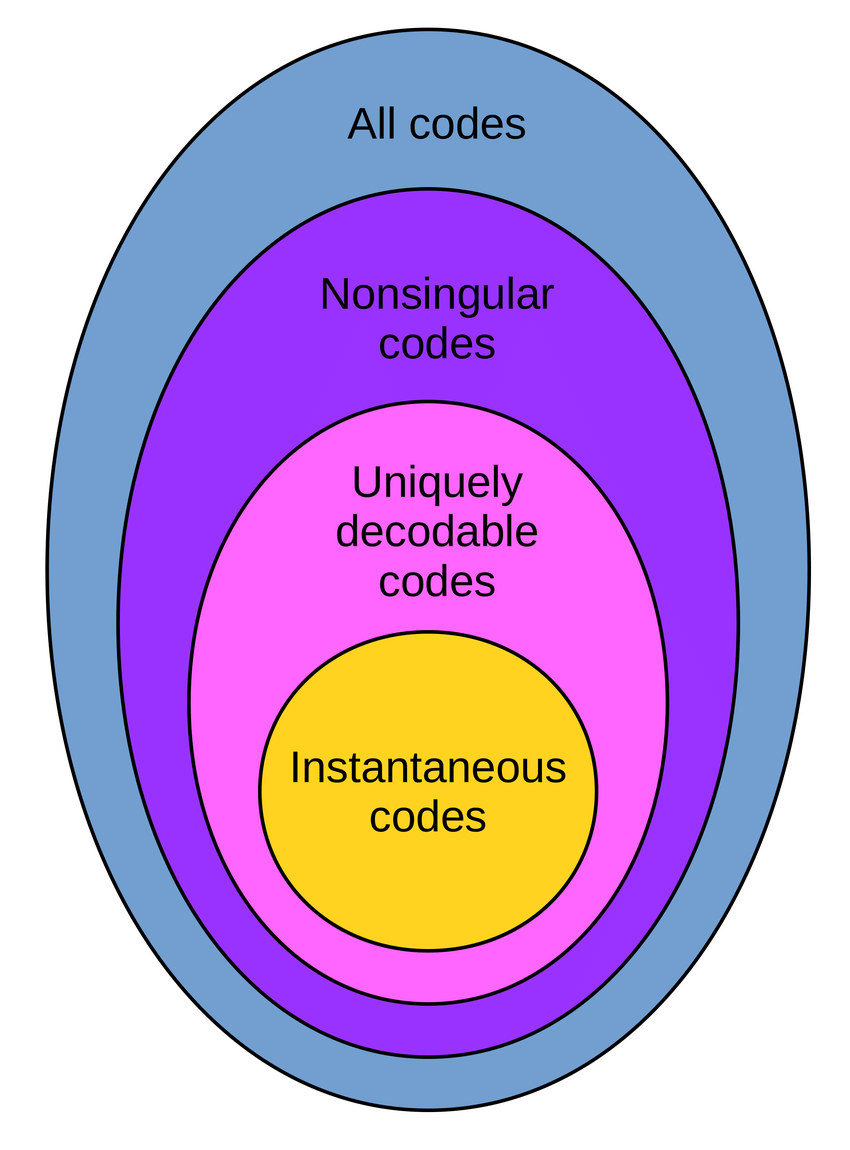
\includegraphics[scale=0.2]{img/codes.png}
\caption{\label{fig:codes} Gerarchia dei codici.}
\end{figure}
\end{minipage}
\begin{minipage}{0.45\textwidth}
Supponendo di avere una sorgente $S$ che emette simboli sull'alfabeto $X = \{a,b,c,d\}$ esaminiamo quattro codici $C: X \to \{0,1\}^*$ e le loro propriet\`a.
\begin{table}[H]
\begin{tabular}{l|l|l|l|l}
\toprule
$X$ & \textcolor{MidnightBlue}{Singolare} & \textcolor{RoyalPurple}{Non-singolare} & \textcolor{Lavender}{UD} & \textcolor{Dandelion}{Istantaneo} \\
\midrule
$a$ & 0         & 0             & 10  & 0          \\
$b$ & 0         & 010           & 00  & 10         \\
$c$ & 0         & 01            & 11  & 110        \\
$d$ & 0         & 10            & 110 & 111        \\
\midrule
    & $C_1$     & $C_2$         & $C_3$ & $C_4$ \\
\bottomrule
\end{tabular}
\label{tab:codici}
\end{table}
In particolare $C_3$ è UD ma non istantaneo perché non rispetta la regola del prefisso: se si riceve $11$ si deve aspettare i bit successivi per sapere se si è effettivamente ricevuto un $c$.
\end{minipage}

\subsection{Disuguaglianza di Kraft-McMillan}
Abbiamo detto che per la codifica di sorgente si è interessati solo ai codici istantanei, ma per ottenerli si devono rispettare  dei vincoli sulla lunghezza dei codici. Non è sempre possibile costruire codici UD e istantanei, ci sono delle condizioni che devono essere verificate. \\
Data una sorgente $S$ con alfabeto $X = \{x_1, x_2, \dots, x_N\}$ e un codice $C$ su un alfabeto\footnote{Nel caso in cui l'alfabeto di codifica sia binario $B = \{0,1\}$ e $|B|=R=2$.} $B = \{b_1, b_2, \dots, b_R\}$ che associa ad ogni simbolo $x_i$ un codice $C(x_i)$ di lunghezza $l_i = l(x_i)$ si ha una 

\textbf{Condizione Necessaria e Sufficiente} (\textbf{\textit{Disuguaglianza di Kraft-McMillan}}): \\
Affinch\`e esista un codice UD e istantaneo con parole di codice lunghe $l_1, l_2, \dots, l_N$ deve essere:
\begin{equation}
    \sum_{i=1}^N R^{-l_i} \leq 1
\end{equation}

Si vede  che  tale  disuguaglianza \textit{considera solo le lunghezze dei codici e niente  altro}. Inoltre, è importante sottolineare  che questo  teorema  dice  solo  che  \textit{se}  questa  condizione  è  soddisfatta sicuramente  \textit{esiste}  un codice univocamente  decodificabile ed istantaneo con queste lunghezze, ma \textit{non dice} che \textit{tutti} i codici con queste lunghezze  sono univocamente  decodificabili  ed istantanei, dice solo che  queste  lunghezze  sono corrette per costruire un univocamente decodificabile ed istantaneo.
\begin{tcolorbox}[enhanced, breakable, frame hidden]
\textbf{Dim}: \\
Dimostriamo prima la \textit{condizione sufficiente}, ovvero che, dati $R, l_1, l_2, \dots, l_N$:
\begin{equation*}
    \sum_{i=1}^N R^{-l_i} \leq 1 \implies \exists \text{ un codice istantaneo con queste lunghezze.}
\end{equation*}
Possiamo pensare, senza perdita di generalit\`a, di ordinare le lunghezze $l_i$ in ordine crescente e di chiamare $l$ la lunghezza massima $l \coloneqq \max \{l_1, l_2, \dots, l_N\}$ con $l > 0$. Quindi si avranno:
\begin{itemize}
    \item $n_1$ parole di codice lunghe $1$, con $n_1 \geq 0$.
    \item  $n_2$ parole di codice lunghe $2$, con $n_2 \geq 0$.
    \item $\dots$
    \item $n_{l-1}$ parole di codice lunghe $l-1$ con $n_{l-1} \geq 0$.
    \item $n_l$ parole di codice lunghe $l$, con $n_l > 0$.
\end{itemize}
Quindi possiamo riscrivere la disuguaglianza come:
\begin{equation*}
    \sum_{i=1}^N R^{-l_i} = \sum_{i=1}^{l} n_i R^{-i} \leq 1
\end{equation*}
Moltiplicando entrambi i membri per $R^l$ si ha che
\end{tcolorbox}
\begin{tcolorbox}[enhanced, breakable, frame hidden]
\begin{equation*}
    R^l \sum_{i=1}^{l} n_i R^{-i} = \sum_{i=1}^{l} n_i R^{l - i} \leq R^l
\end{equation*}
decomponendo la somma si ha
\begin{equation*}
    n_1 R^{l-1} + n_2 R^{l-2} + \dots +n_{l-2}R^2 + n_{l-1}R + n_l \leq R^l
\end{equation*}
isolando $n_l$ si ottiene
\begin{equation*}
    n_l \leq R^l - n_1 R^{l - 1} - n_2 R^{l - 2} - \dots - n_{l-1} R 
\end{equation*}
ma, essendo $n_l > 0$, anche 
\begin{equation*}
    0 < R^l - n_1 R^{l - 1} - n_2 R^{l - 2} - \dots - n_{l-1} R 
\end{equation*}
da cui
\begin{align*}
    &n_{l-1} R < R^l - n_1 R^{l - 1} - n_2 R^{l - 2} - \dots - n_{l-2}R^2 \\
    &n_{l-1} < R^{l-1} - n_1 R^{l-2} - n_2 R^{l -3} - \dots - n_{l-2}R
\end{align*}
Ricordando che $n_{l-1} \geq 0$ si ha
\begin{align*}
    &0 < R^{l-1} - n_1 R^{l-2} - n_2 R^{l-3} - \dots - n_{l-2}R \\
    &n_{l-2}R < R^{l-1} - n_1 R^{l-2} - n_2 R^{l-3} - \dots - n_{l-3}R^2 \\
    &n_{l-2} < R^{l-2} - n_1 R^{l-3} - n_2 R^{l-4} - \dots n_{l-3}R
\end{align*}
Proseguendo in questo modo fino a $n_1$ si ottiene
\begin{align*}
\begin{cases}
n_l \leq R^l - n_1 R^{l - 1} - n_2 R^{l - 2} - \dots - n_{l-1} R \\
n_{l-1} < R^{l-1} - n_1 R^{l-2} - n_2 R^{l -3} - \dots - n_{l-2}R \\
n_{l-2} < R^{l-2} - n_1 R^{l-3} - n_2 R^{l-4} - \dots n_{l-3}R \\
\dots \\
n_3 < R^3 - n_1 R^2 - n_2 R \\
n_2 < R^2 - n_1 R \\
n_1 < R
\end{cases}
\end{align*}
Quindi, ricapitolando, se vale la condizione di Kraft-McMillan sulle lunghezze $l_i$ si ha che valgono queste disequazioni, che altro non sono che la definizione alternativa di un codice istantaneo. \\
Dimostriamo ora la \textit{condizione necessaria}, ovvero che per un codice univocamente decodificabile (quindi anche per uno istantaneo$^{\ref{fig:codes}}$) con lunghezze $\{l_1, l_2, \dots, l_N\} \implies \sum_{i=1}^N R^{-l_i} \leq 1$. \\
Si ha
\begin{equation*}
    \Big ( \sum_{i=1}^N R^{-l_i} \Big )^n = \underbrace{\sum_{i=1}^N R^{-l_i} \sum_{j=1}^N R^{-l_j} \dots \sum_{k=1}^N R^{-l_k}}_n = \sum_{i=1}^N \sum_{j=1}^N \dots \sum_{k=1}^N R^{-(l_i + l_j + \dots + l_k)}
\end{equation*}
\end{tcolorbox}
\begin{tcolorbox}[enhanced, breakable, frame hidden]
Si ha che $p \coloneqq l_i + l_j + \dots l_k$ non \`e altro che la somma delle lunghezze di $n$ parole di codice. Chiamando come prima $l \coloneqq \max \{l_1, l_2, \dots, l_N\}$ si ha che $p \in [n, nl]$ (ovvero \`e compreso tra la somma di $n$ parole lunghe 1 ed $n$ parole lunghe $l$) da cui, chiamando $L_p$ il numero di concatenazioni di $n$ parole di codice le cui lunghezze sommate danno $p$, si ha:
\begin{equation*}
    \Big ( \sum_{i=1}^N R^{-l_i} \Big )^n = \sum_{i=1}^N \sum_{j=1}^N \dots \sum_{k=1}^N R^{-(l_i + l_j + \dots + l_k)} = \sum_{p=n}^{nl} L_p R^{-p}
\end{equation*}
Ma  la concatenazione  di $n$ parole di codice  non  è  altro  che la parola di codice  di  un  messaggio  di $n$ simboli, cio\`e  un  codice dell’estensione $n$-esima della sorgente $S^n$. Per definizione di univocamente decodificabile, quindi, qualunque sia l’estensione della sorgente ($\forall n$) si ha che presi due codici questi devono essere diversi. \\
Questo implica che, se abbiamo $L_p$ codici di lunghezza $p$, per fare in modo che siano diversi tra loro deve valere
\begin{equation*}
    L_p \leq R^p
\end{equation*}
Da cui:
\begin{align*}
    &\Big ( \sum_{i=1}^N R^{-l_i} \Big )^n = \sum_{p=n}^{nl} L_p R^{-p} \leq \sum_{p=n}^{nl} R^p R^{-p} = \sum_{p=n}^{nl} 1 = nl - n + 1  \leq nl
\end{align*}
quindi
\begin{equation*}
    \Big ( \sum_{i=1}^N R^{-l_i} \Big )^n \leq nl \implies \sum_{i=1}^N R^{-l_i} \leq 1
\end{equation*}
Infatti se fosse $ \sum_{i=1}^N R^{-l_i} > 1$ (quindi $\sum_{i=1}^N R^{-l_i} = 1 + \epsilon$) si avrebbe che, ad esempio
\begin{equation*}
\lim_{n \to \infty} \frac{(1+\epsilon)^n}{n} = \infty \nleq l
\end{equation*}

$\square$
\end{tcolorbox}

\subsection{Codici compatti}
Siamo adesso interessati a definire codici \textit{efficienti}. Iniziamo con una definizione:
\defn{\textit{Codice compatto:}} Un codice $\mathcal{C}$ si definisce compatto se: 
\begin{enumerate}
    \item \`E univocamente decodificabile.
    \item La sua lunghezza media $L_{\mathcal{C}}$ \`e la minore tra tutti gli altri codici UD per la sorgente $S$ sull'alfabeto $B$.
    \[
    L_{\mathcal{C}} \leq L_C, \quad \forall C: X \to B^*
    \]
\end{enumerate}
Per trovare codici compatti dobbiamo capire quale è la \textit{minima lunghezza possibile} di un codice. Assumendo momentaneamente che la sorgente $S$ sia una DMS (rilasseremo poi quest'ipotesi alle sorgenti di Markov) abbiamo un risultato molto importante. Si ha che, detta $H_b (S)$ l'entropia della sorgente $S$ in base $b$, 
\begin{equation}
    \frac{H(S)}{\log b} = H_b (S) \leq L
\end{equation}
ovvero che l'entropia della sorgente rappresenta un limite inferiore per la lunghezza media di un codice univocamente decodificabile. Questo  è  un  primo  importante  risultato  perché  \textit{lega  la  definizione  di  informazione/entropia  con  una quantità che non dipende dalla definizione stessa di informazione}.\\
Se, per un codice UD $\mathcal{C}$, vale il limite inferiore $H_b(S) = L_{\mathcal{C}}$ allora il codice \`e un \textbf{codice compatto}. Questo avviene quando $\forall x \in X, \exists l \in \mathbb{N}:$
%\begin{equation*}
%    H_b(S) = \sumx p(x) \log_b \frac{1}{p(x)} = \sumx p(x) l(x) = L_{\mathcal{C}} \implies \log_b  %\frac{1}{p(x)} = l(x) \implies  p(x) = b^{-l(x)}
%\end{equation*}
%cio\`e quando, 
\begin{equation*}
   p(x) = b^{-l}
\end{equation*}
nel caso in cui $b=2$ la sorgente si dice \textit{diadica}.
\begin{tcolorbox}[enhanced, breakable, frame hidden]
\textbf{Dim}: Dimostriamo che $H(S)-L \leq 0$, il caso generale non \`e molto diverso.
\begin{align*}
    H(S) - L &= \sumx p(x) \info{x} - \sumx p(x) l(x) = \\
    &= \sumx p(x) \info{x} - \sumx p(x) \log 2^{l(x)} = \\
    &= \sumx p(x) \log \frac{2^{-l(x)}}{p(x)} = \log e \sumx p(x) \ln \frac{2^{-l(x)}}{p(x)} \leq \\
    &\leq \log e \sumx p(x) \Big ( \frac{2^{-l(x)}}{p(x)} - 1 \Big ) = \\
    &=\log e \bigg ( \underbrace{\sumx 2^{-l(x)}}_{\leq 1} - \sumx p(x) \bigg ) \leq 0
\end{align*}
Inoltre l'uguaglianza vale quando le due disuguaglianze valgono con l'uguaglianza, cio\`e quando:
\begin{equation*}
\begin{cases}
\frac{2^{-l(x)}}{p(x)} = 1 \iff p(x) = 2^{-l(x)}, \hspace{5pt} \forall x \in X \\
\sumx 2^{-l(x)} = 1
\end{cases}
\end{equation*}
\hspace{400pt}$\square$
\end{tcolorbox}
Quindi, per una DMS in cui le probabilità di emissione siano della forma (generale), $\forall x \in X$
\begin{equation*}
    p(x) = b^{-l(x)} =  \Big ( \frac{1}{b} \Big )^{l(x)}
\end{equation*}
si può avere una lunghezza  di  codice  (istantaneo) \textit{minima pari all’entropia della  sorgente stessa}. Ovviamente  avere probabilità di questa forma non è realistico. Consideriamo allora il caso di una sorgente DMS in cui i valori di $p(x)$ siano arbitrari, quindi non rispettano nessun vincolo. Questo implica che $H_b(S) < L$, ovvero non si può più avere un codice di lunghezza minima possibile. 
\defn{\textit{Efficienza:}} Si definisce l'efficienza $\eta$ di un codice con lunghezza media $L$ per una sorgente $S$ come:
\begin{equation}
    \eta \coloneqq \frac{H_b(S)}{L}
\end{equation}
Quanto pi\`u questo numero (puro) si avvicina a $1$ tanto maggiore \`e l'efficienza della codifica. 
\subsection{Primo Teorema di Shannon}
Shannon ha  studiato  come  cercare  di  avvicinarsi  al  limite  minimo  anche  in  caso  in  cui le  probabilità  di emissione dei simboli siano arbitrarie. Ha pensato, nel caso in cui i valori di $p(x)$ siano arbitrari, di approssimare $l(x)$ con l’intero maggiore più vicino a quello di una sorgente diadica\footnote{In una sorgente diadica si ha, equivalentemente, $l(x) = \log_b p(x)^{-1}= -\log_b p(x)$}, cio\`e, $\forall x \in X$:
\begin{equation}
l_S(x) \coloneqq \bigg \lceil \log_b \frac{1}{p(x)} \bigg \rceil
\end{equation}
Si ha ovviamente che, $\forall x \in X$
\begin{equation}
    l(x) \leq l_S(x) \leq l(x) + 1
\end{equation}
e che il codice costruito con queste lunghezze \`e istantaneo, soddisfando la disugaglianza di Kraft-McMillan. Considerando infatti la prima delle due disugaglianze $l(x) \leq l_S(x)$ vale
\begin{align*}
    &l(x) = \log_b \frac{1}{p(x)} \leq l_S(x) \implies \frac{1}{p(x)} \leq b^{l_S(x)} \implies \\
    &\implies p(x) \geq b^{-l_S(x)} \implies \sumx p(x) = 1 \geq \sumx b^{-l_S(x)}
\end{align*}
Inoltre si ha che 
\begin{equation}
    H_b(S) \leq L \leq H_b(S) + 1
\end{equation}
\begin{tcolorbox}[enhanced, breakable, frame hidden]
\textbf{Dim}: Dimostriamo nel caso $b=2$. Si ha
\begin{align*}
    &\log \frac{1}{p(x)} \leq \hspace{2pt} l_S(x) \leq \info{x} + 1 \text{ da cui}\\
    &\underbrace{\sumx p(x) \info{x}}_{=H(S)} \leq \underbrace{\sumx p(x) l_S(x) }_{=L} \leq \sumx p(x) \Big ( \info{x} + 1 \Big ) = H(S) + 1 \\
    &\hspace{400pt}\square
\end{align*}
\end{tcolorbox}

\subsubsection{Sorgenti discrete senza memoria}
Shannon ha osservato che, estendendo la sorgente e codificando i messaggi invece dei singoli simboli la lunghezza media per codificare un simbolo si riduce.
Basandoci su questa osservazione si consideri la sorgente estesa $S^n$ in cui vengono inviati messaggi $\sigma_i$ di $n$ simboli appartenenti all'alfabeto $X = \{x_1, x_2, \dots, x_M\}$:
\begin{equation*}
    \sigma_i = \{ x_{i_1} x_{i_2} \dots x_{i_n} \}
\end{equation*}
Si hanno quindi $M^n$ possibili messaggi $\sigma$ emittibili dalla sorgente estesa $S^n$ caratterizzati da una probabilit\`a $p(\sigma)$. Scegliendo, seguendo la codifica di Shannon, un codice di lunghezza
\begin{equation}
    \lambda(\sigma) = \Big \lceil \log \frac{1}{p(\sigma)} \Big \rceil
\end{equation}
si ha, come prima
\begin{equation*}
   \log \frac{1}{p(\sigma)} \leq \lambda(\sigma) \leq \log \frac{1}{p(\sigma)} + 1
\end{equation*}
da cui, mediando su tutti gli $M^n$ messaggi $\sigma \in S^n$, si ottiene
\begin{equation}
    \sum_{\sigma \in S^n} p(\sigma) \log \frac{1}{p(\sigma)} \leq \sum_{\sigma \in S^n} p(\sigma) \lambda(\sigma) \leq \sum_{\sigma \in S^n} p(\sigma) \Big ( \log \frac{1}{p(\sigma)} + 1 \Big )
\end{equation} da cui
\begin{equation}
    H(S^n) \leq L_n \leq H(S^n) + 1
\end{equation}
in cui si \`e definito
\begin{equation}
    L_n \coloneqq \sum_{\sigma \in S^n} p(\sigma) \lambda(\sigma)
\end{equation}
ovvero la lunghezza media del codice per simbolo esteso (il numero medio di simboli dell’alfabeto di codice) quando si mandano e si decodificano $n$ simboli consecutivi.
Ricordando poi che $H(S^n) = nH(S)$ si ottiene
\begin{equation}
    H(S) \leq \frac{L_n}{n} \leq H(S) + \frac{1}{n}
\end{equation}
Si ha quindi che $L_n / n$, cio\`e il numero medio di simboli del codice usati per codificare un blocco di $n$ simboli, tende a $H(S)$ all'aumentare di $n$. \\
Si ha quindi il \textbf{Primo Teorema di Shannon per una DMS}: \textit{possiamo codificare una sorgente senza memoria con una lunghezza media per simbolo vicina a piacere al limite minimo (l'entropia della sorgente) codificando più simboli insieme invece che uno solo.} \\
Il prezzo che si paga è la complessità, dovendo codificare e decodificare $n$ simboli consecutivi lavorando con la sorgente estesa $S^n$.
\subsubsection{Sorgenti di Markov}
Sia ora $S$ una sorgente discreta con memoria di Markov. Quanto visto precedentemente per le sorgenti DMS in merito alla minima lunghezza di codifica vale anche per le sorgenti con memoria. Se infatti consideriamo $\bar{S}$, la sorgente aggiunta di $S$, essendo questa senza memoria vale quando già visto ovvero $H(\bar{S}) \leq L$. Ma vale anche $H(S) \leq H(\bar{S})$ da cui
\begin{equation}
    H(S) \leq L
\end{equation}
Possiamo estendere il Primo Teorema di Shannon alle sorgenti con memoria di Markov. \\
Per una sorgente di Markov $S$ di ordine 1 si ha
\begin{equation}
    H(S) + \frac{H(\bar{S}) - H(S)}{n} \leq \frac{L_n}{n} \leq H(S) + \frac{H(\bar{S}) - H(S)}{n} + 1
\end{equation}
mentre in generale per una sorgente di Markov di ordine $k$ vale, per un certo $\epsilon_k \in \mathbb{R}$
\begin{equation}
    H(S) + \frac{\epsilon_k}{n} \leq \frac{L_n}{n} \leq H(S) + \frac{\epsilon_k}{n} + 1
\end{equation}
\begin{tcolorbox}[enhanced, breakable, frame hidden]
\textbf{Dim}: Dimostriamo nel caso di una sorgente di Markov di ordine $1$. \\
Consideriamo l'aggiunta di $S$, ovvero la sorgente $\bar{S}$, si ha che, essendo questa una DMS, scelto $\forall x \in X$ un codice di Shannon dato da $l(x) = \lceil - \log p(x) \rceil$ (dove $p(x)$ \`e la probabilit\`a incondizionata), vale
\begin{equation*}
    H(\bar{S}) \leq L \leq H(\bar{S}) + 1
\end{equation*}
Si può quindi prendere la sorgente aggiunta $\overline{S^n}$ della sorgente estesa e arrivare esattamente come prima a scrivere
\begin{equation*}
    H(\overline{S^n}) \leq L_n \leq H(\overline{S^n}) + 1
\end{equation*}
Ricordando poi, dalla \ref{eqn:adjmarko}, che per una sorgente di Markov del primo ordine si ha
\begin{equation*}
    H(\overline{S^n}) = nH(S) + [H(\bar{S}) - H(S)]
\end{equation*}
da cui
\begin{equation*}
    H(S) + \frac{H(\bar{S}) - H(S)}{n} \leq \frac{L_n}{n} \leq H(S) + \frac{H(\bar{S}) - H(S)}{n} + 1
\end{equation*}
Per le sorgenti di Markov di ordine superiore l’espressione è analoga perché vale
\begin{equation*}
  \hspace{70pt}  H(\overline{S^n}) = nH(S) + \epsilon_k, \hspace{50pt} \square
\end{equation*}
\end{tcolorbox}

\newpage
\section{Rate-Distortion Theory} \label{sec:rdt}
Il primo teorema di Shannon si riferisce a codifica senza perdita e a sorgenti discrete. Quando si ha a che fare
con la codifica lossless, non ci si deve preoccupare di come avverrà la ricostruzione dell’informazione dopo
la decodifica perché sappiamo che il processo è completamente reversibile, quindi la ricostruzione in
decodifica è identica all’originale. Tuttavia, Shannon ci dice che se vogliamo preservare tutta l’informazione
della sorgente, la capacità di compressione ha un limite fondamentale che è dato dall’entropia. \\
In alcuni casi ed applicazioni la compressione lossless può andare bene, ma in altri può essere necessario aumentare il tasso di compressione accettando un certo livello di perdita di informazione, ovvero facendo una codifica \textit{lossy}. Inoltre si deve tenere in considerazione che quando la sorgente informativa è analogica per
trasformarla in numerica si effettua \textit{sempre} una codifica di sorgente lossy.

Se nella codifica lossless l’unica metrica di interesse è il \textit{rate di generazione} $R$, ovvero il \textbf{numero di bit per simbolo necessari a rappresentare la sorgente}, nella codifica lossy questo non basta, infatti se così fosse, la migliore forma di codifica sarebbe buttare via tutti i dati. \\
Quando si ha codifica lossy ci interessa quindi il rate ma anche la perdita di informazione, ovvero una misura della differenza tra l’informazione originaria e quella ricostruita. La perdita dell’informazione viene denominata \textbf{distorsione}.

La \textit{distorsione} $D$ è tanto maggiore tanto pi\`u i dati ricostruiti, a valle della compressione, distano in qualità dai dati originali. Il concetto di qualità (distorsione accettabile) non è un concetto assoluto, ma dipende necessariamente dall’\textit{applicazione} dei dati, e cioè dall’impiego che si fa dei dati ricostruiti e da chi ne usufruisce. \\
Si hanno diversi modi di misurare la distorsione e la qualità di un segnale ricostruito e diversi livelli di distorsione accettabili. In ogni caso, comunque sia definita la misura della distorsione, ci\`o che si desidera è trovare una tecnica di codifica che per ogni fissato livello di distorsione $D$ codifichi la sorgente al tasso $R$ più piccolo possibile (o, al contrario, che per ogni fissato tasso di codifica $R$ comporti la minima distorsione $D$).

La Rate-Distortion Theory è il ramo della teoria dell’informazione che descrive il \textit{trade-off} tra il rate di trasmissione (bit/simbolo usati per la codifica) e la corrispondente distorsione e fornisce i limiti per la compressione con perdita. Si sottolinea come questa sia essenziale per sorgenti continue per le quali non \`e possibile avere una codifica lossless. \\
La Rate-Distortion Theory si occupa quindi di trovare le prestazioni limite teoriche, in termini di funzioni $R(D)$ e $D(R)$ per assegnate sorgenti e misure di distorsione.
A livello pratico si vuole
\begin{itemize}
    \item Definire un modo per misurare la distorsione $D$.
    \item Determinare il rate minimo (massima compressione) $R$ a cui si può lavorare ammettendo una certa distorsione o, equivalentemente, la distorsione minima che si ha lavorando con un certo rate.
\end{itemize}
Come nel caso della codifica lossless la teoria dell’informazione fornisce dei limiti teorici che poi servono per
la progettazione delle tecniche di codifica. Tuttavia in caso di codifica con perdita, anche per sorgenti
piuttosto semplici, esistono pochi risultati in forma chiusa della rate-distortion theory, e si dovr\`a quindi ricorrere ad approssimazioni. Inoltre, anche quando le curve limite sono note, i metodi di codifica esistenti forniscono prestazioni lontane da quelle ottime, soprattutto a causa dei vincoli di memoria e complessità computazionale ai quali si deve sottostare.
\begin{figure}[H]
    \centering
    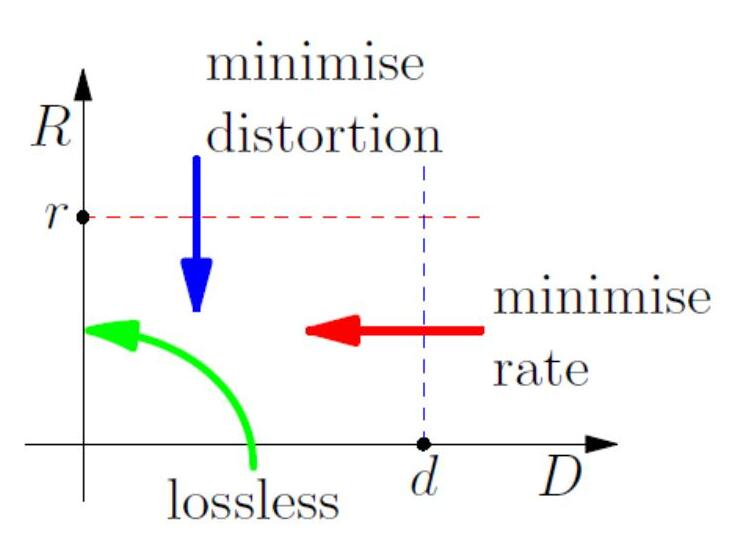
\includegraphics[scale=0.2]{img/rdt.jpg}
    \caption{Obiettivo della RDT.}
    \label{fig:rtd}
\end{figure}

\subsection{Distorsione}
Dato che la valutazione della qualità della codifica dipende dall’uso che si deve fare dei dati codificati non è possibile definire un metodo di misura universalmente valido. Si deve scegliere allora il metodo che di volta in volta risulta più adatto all’applicazione. Sia $x \in X$ un elemento dell'alfabeto della sorgente e sia $\hat{x} \in \hat{X}$ l'elemento stesso ricostruito dal ricevitore. Dovendo quantificare la distorsione dovremo avere che questa sia, in qualche modo, funzione di una distanza $d(\cdot, \cdot)$ tra i due oggetti. Vediamo due metriche di distanza per variabili aleatorie:
\begin{enumerate}
    \item Nel caso di sorgenti binarie una misura comunemente usata è la \textit{Distanza di Hamming:} \begin{equation}
        d(x, \hat{x}) = x \oplus \hat{x} \coloneqq \begin{cases}
        0, & \text{se } x = \hat{x} \\
        1, & \text{se } x \neq \hat{x}
        \end{cases}
    \end{equation}
    \item Nel caso di sorgenti continue il modo più naturale per vedere la fedeltà della ricostruzione è fare la differenza tra i valori iniziali e quelli ricostruiti. Il più popolare è l’\textit{errore quadratico} (SE):
    \begin{equation*}
        d(x, \hat{x}) = (x - \hat{x})^2
    \end{equation*}
\end{enumerate}
Ovviamente può essere definita anche in altro modo, ad esempio come la differenza assoluta tra due campioni. In
generale, la cosa migliore di tutti sarebbe tener conto dell’effetto finale della distorsione, ovvero come questa
viene percepita: tale valutazione non è per\`o una misura oggettiva, ma dipendente dal contesto e quindi per poterla effettivamente quantificare si deve ricorrere a misure come l’MSE che non sono perfette ma semplici e oggettive. Ad esempio nel caso della trasmissione di segnali vocali anche se l'MSE è alto si può avere una buona percezione, ovvero che la distorsione percepita è bassa.
\defn{\textit{Distorsione:}} La distorsione $D$ \`e definita come
\begin{equation}
    D = \mathbb{E} [ d(X, \hat{X})]
\end{equation}
dove la media viene fatta su tutti gli elementi dell'alfabeto $X$ e su tutti i possibili simboli ricostruiti dell'alfabeto $\hat{X}$, quindi sulla distribuzione congiunta $p(x, \hat{x})$.\\
Nei due casi precedenti quindi si ha
\begin{itemize}
    \item La probabilit\`a di ricostruire in modo sbagliato $D = \mathbb{E} [X \oplus \hat{X}] \coloneqq P_e$
    \item Il Mean Squared Error (MSE) dato da $D = \mathbb{E} [(X - \hat{X})^2]$
\end{itemize}
La distorsione con la distanza di Hamming prende il nome di \textit{probability of a reconstruction error} dal momento che $\mathbb{E}[X \oplus \hat{X}] = 0 \times Pr\{x=\hat{x}\} + 1 \times Pr\{x \neq \hat{x}\} = P_e$.\\
Estendendo alle sequenze di simboli $x^n, \hat{x}^n$ si ha
\begin{equation}
    d(x^n, \hat{x}^n) = \frac{1}{n} \sum_{i=1}^n d(x_i, \hat{x}_i)
\end{equation}
che, nel caso di sorgenti stazionarie (\textit{i.i.d}), porta allo stesso valor medio
\begin{equation}
    D = \mathbb{E} [d(X^n, \hat{X}^n) = \mathbb{E}[d(X, \hat{X})]
\end{equation}
Si pu\`o definire anche un'altra importante grandezza: il rapporto segnalre-rumore (\textbf{SNR}). Il rapporto segnale-rumore è un numero puro o adimensionale, dato dal rapporto fra due grandezze omogenee, che esprime quanto il segnale sia \textit{più potente} del rumore nel sistema considerato. È formalmente espresso dalla relazione: 
\begin{equation}
    SNR = \frac{\sigma_x^2}{\sigma_d^2}
\end{equation}
dove $\sigma_x^2$ rappresenta la potenza del segnale utile e $\sigma_d^2$ la potenza totale del rumore presente nel sistema (dato dalla distorsione). Queste vengono solitamente espresse in $Watt$ o $dBm$. Più basso è l'SNR, più sarà difficoltosa la decodifica del segnale ovvero più alta sarà la probabilità di errore.

\subsection{Funzione di Rate-Distortion}
Data una distribuzione statistica della sorgente e una misura della distorsione $D$, la domanda a cui si prova
a rispondere è \emph{quale è la minima distorsione $D$ ottenibile quando viene fissata una velocità di trasmissione $R$?} La funzione di Rate-Distortion $R(D)$ fornisce il numero minimo di bit (cio\`e il rate minimo $R$) che si può usare per rappresentare una sorgente e che garantisce un errore di ricostruzione
\begin{equation}
    \mathbb{E} [d(X, \hat{X})] \leq D
\end{equation}
Il caso $D = 0$ significa che non viene accettata distorisione da cui $R(0)$ nel caso di sorgenti discrete coincide con l'entropia della sorgente $H(X)$ e, nel caso di sorgenti continue, $R(0) = \infty$. \\
$R(D)$ è una funzione monotona decrescente di $D$. Equivalentemente potremmo anche determinare l'inversa $D(R)$, rispondendo alla domanda \emph{qual è la velocità minima (numero minimo di bit per
la rappresentazione) che si può avere per garantire una data distorsione?} In questo caso la funzione inversa
$D(R)$ (Distortion-Rate) fornisce il livello di distorsione del segnale riscostruito fissato il massimo numero di bit che si possono spendere per la rappresentazione.
\begin{figure}[H]
    \centering
    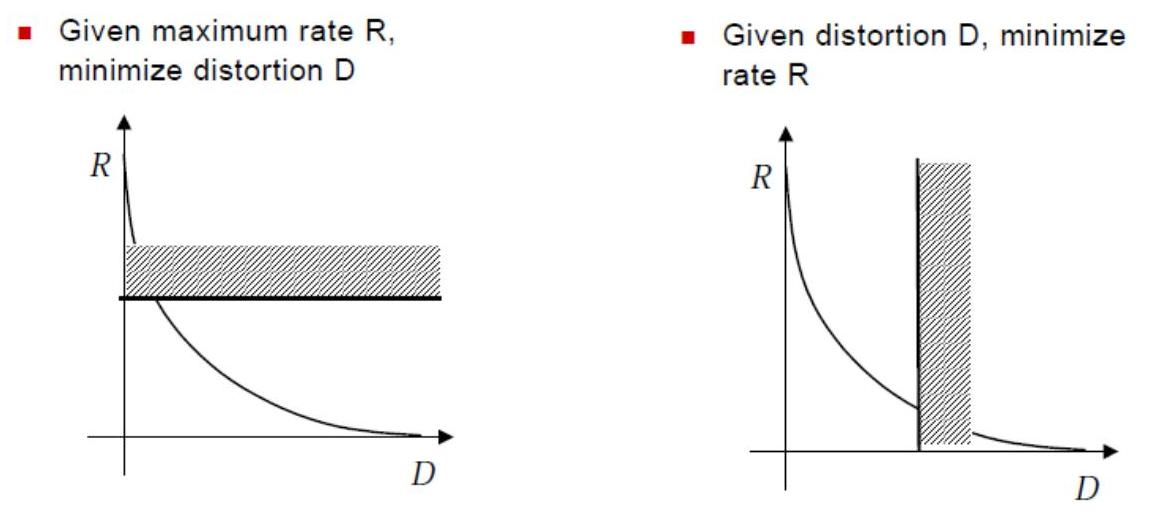
\includegraphics[scale=0.2]{img/rdf.jpg}
    %\caption{Rate-Distorsion}
    \label{fig:rdf}
\end{figure}
\defn{\textit{Raggiungibilit\`a:}} Una coppia $(R,D)$ si dice raggiungibile se esiste una codifica a rate $R$ tale che
\begin{equation}
    \lim_{n \to \infty} \frac{1}{n} \sum_{i=1}^n d(x_i, \hat{x}_i) \leq D
\end{equation}
La \textbf{regione di rate-distortion} $\mathcal{R}$ rappresenta l’insieme dei punti $(R,D)$ raggiungibili e la funzione di rate distortion è l’estremo inferiore dei rate $R$ tali che $(R,D) \in \mathcal{R}$ per ciascun valore di $D$ fissato. \\
La funzione di rate-distortion $R(D)$ è quindi il \textit{lower-bound del rate di trasmissione per un fissato valore di distorsione $D$:} Se $R > R(D)$ allora esiste una sequenza di codici con una distorsione media che si avvicina a $D$, altrimenti se il rate \`e nella zona inferiore, tali codici non esistono.
\begin{figure}[H]
    \centering
    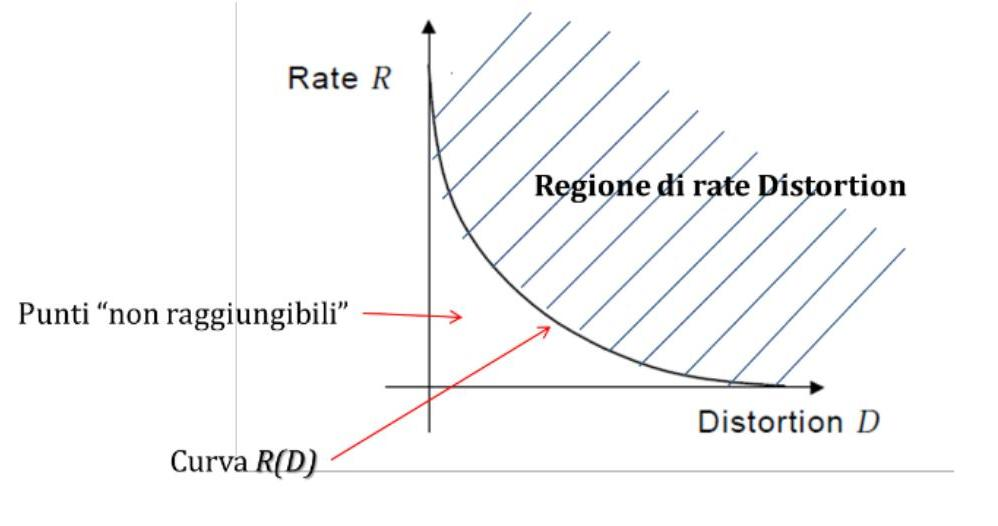
\includegraphics[scale=0.3]{img/rdc.jpg}
    \caption{Regione di rate distortion.}
    \label{fig:rdc}
\end{figure}
Il principale Teorema della Rate Distortion Theory \`e dovuto a Shannon (1956) ed \`e noto come \textit{Lossy Coding Theorem} (Teorema della Codifica con Perdita):

\textbf{Teorema}: Sia $(X,\hat{X}) \sim p(x, \hat{x})$ con allora la funzione $R(D)$ per la sorgente\footnote{La stessa definizione vale nel caso continuo utilizzando le funzioni densità di probabilità.} $X$ con simboli \textit{i.i.d.} e funzione di distanza $d(x, \hat{x})$ \`e data da
\begin{align*}
    R(D) = &\min_{p(x|\hat{x})} I(X; \hat{X}) \\
    &\text{s.t. } \mathbb{E}[d(X, \hat{X})] \leq D
\end{align*}
Fissata un valore di distorsione $D$, il minimo rate $R$ possibile si trova minimizzando l’informazione muta, tra tutte le coppie $(x, \hat{x})$ (e quindi tra tutte le possibili codifiche $\hat{x} = C(x)$) che soddisfano $D$. Si noti come il vero grado di libert\`a nella minimizzazione sia la distribuzione condizionata $p(\hat{x}|x)$, derivante dal fatto che la minimizzazione avvenga su $p(x, \hat{x}) = p(\hat{x}|x)p(x)$ in cui $p(x)$ dipende dalla sorgente mentre $p(\hat{x}|x)$ descrive la codifica ed \`e quello che ci permette di minimizzare $I(X; \hat{X})$.\\
L’informazione mutua tra due sorgenti ci dice quanto di una sorgente è contenuto nell’altra, in questo caso
quanto dell’informazione originaria è contenuta in quella ricostruita, dopo la codifica/decodifica con perdita. 

Ricapitolando: più la codifica comprime (più si riducono i bit di rappresentazione $R$) e più si perde informazione. Si avrà quindi sempre meno informazione di $X$ contenuta in $\hat{X}$ e $I(X; \hat{X})$ diminuir\`a. Quest'ultima per\`o può diminuire solo fino al limite in cui garantisce il vincolo sulla distorsione $D$, restringendo quindi l'insieme di coppie ($X, \hat{X})$ ammissibili.

Se si ha una sorgente continua  e la si quantizza questa  è  una  forma  di  codifica  con  perdita: fissata  la  massima distorsione che si vuole avere (che corrisponde all’errore di quantizzazione) si fissano i livelli di quantizzazione, e quindi i bit di rappresentazione, e quindi il rate.

\begin{mybox}{green}{\textit{\textbf{Esempio 1} : \textbf{R(D) per una sorgente gaussiana. }}}
Sia $X \sim \mathcal{N}(0, \sigma^2)$. Per questo genere di sorgenti \`e ragionevole adottare la distanza a errore quadratico. La funzione di rate distortion $R(D)$ \`e data da
\begin{equation*}
    R(D) = \begin{cases}
    \frac{1}{2} \log \frac{\sigma^2}{D} & \text{se } 0 \leq D \leq \sigma^2 \\
    0 & \text{se } D > \sigma^2
    \end{cases}
\end{equation*}
Dal momento che la funzione \`e invertibile in $[0, \sigma^2]$ si ha
\begin{equation*}
    D(R) = \sigma^2 2^{-2R}
\end{equation*}
infatti 
\begin{equation*}
    2^{R(D)} = 2^{\frac{1}{2} \log (\frac{\sigma^2}{D})} = 2^{\log \frac{\sigma}{\sqrt{D}}} = \frac{\sigma}{\sqrt{D}} \implies \sqrt{D} = \frac{\sigma}{2^R} \implies D = \sigma^2 2^{-2R}
\end{equation*}
Inoltre il $SNR$ associato alla distorsione \`e dato da
\begin{equation*}
    SNR = \frac{\sigma^2}{D} = 2^{2R}
\end{equation*}
da cui
\begin{equation*}
    SNR_{db} \approx 6R
\end{equation*}
ovvero, se si aumenta di 1 bit il rate (si rappresenta con un bit in più i simboli della sorgente in media) la
distorsione si riduce di $\frac{1}{2^2}$ cio\`e di circa $6 db$.
\end{mybox}

\subsection{Rate-Distortion Bounds}
Spesso non è possibile trovare la funzione di Rate-Distortion per sorgenti con distribuzione qualsiasi. In questi casi è quindi utile avere dei limiti (superiori ed inferiori) che forniscono comunque un range di valori “raggiungibili”, che quindi possono essere presi a riferimento per la progettazione e per valutare margini di miglioramento. \emph{In questo modo la funzione di rate-distortion gioca lo stesso ruolo per la compressione con perdita dell’entropia nel caso di quella senza perdita.}

Si può dimostrare che per una generica sorgente continua con pdf $f_X(x)$ a media nulla e varianza $\sigma^2$, se la distorsione \`e misurata come un MSE, allora vale
\begin{equation}
    h(x) - \frac{1}{2} \log (2\pi e D) \leq R(D) \leq \frac{1}{2} \log \frac{\sigma^2}{D}
\end{equation}
Per una variabile aleatoria gaussiana questi due bound coincidono.
\subsection{Quantizzazione}
\textit{Quando la sorgente d’informazione è continua, il processo di acquisizione dei dati è un processo con perdita di informazione:} l’informazione deve essere discretizzata attraverso il del campionamento e i valori continui devono essere rappresentati con una stringa \textit{finita} di simboli binari. La perdita di informazione dovuta alla quantizzazione è inevitabile quando si passa da sorgenti continue a sistemi digitali, però è una perdita controllata, e può essere usata per diminuire la quantità di dati da gestire (ovvero diminuire il rate del segnale).

\begin{center}
\emph{“The question is: can we assign a definite rate to a continuous source when we require only a certain fidelity of recovery, measured in a suitable way?”}\\
Shannon, A Mathematical Theory of Communication.
\end{center}

Per la progettazione di un quantizzatore quindi la questione è \textit{come trovare la migliore possibile
rappresentazione} di una sorgente continua dato un certo rate di trasmissione $R$. Esistono vari tipi di
quantizzatori e ciascuno porta ad un certo valore di $D$.\\
In generale la quantizzazione è un processo molto semplice: si rappresentano tutti i possibili valori assunti
dai simboli sorgente, con un ben più ristretto set di valori.
\begin{figure}[H]
    \centering
    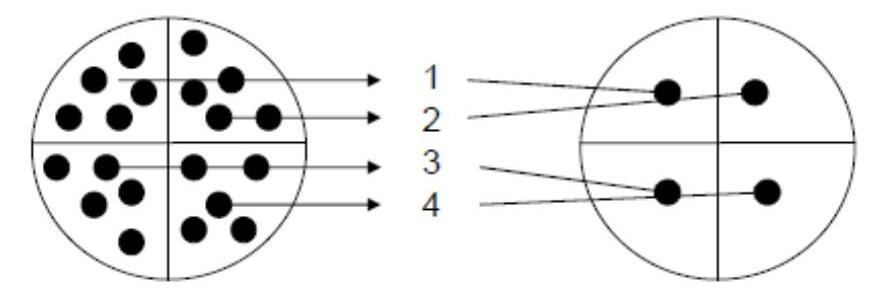
\includegraphics[scale=0.2]{img/quant.jpg}
    \caption{Perdita della iniettivi\`a.}
    \label{fig:quant}
\end{figure}
Il quantizzatore divide il range di valori che una sorgente genera in un numero finito di intervalli ciascuno dei quali è rappresentato da un \textit{valore di riferimento} e poi da una parola di codice (binaria): infiniti valori possono cadere nello stesso intervallo e quindi il processo è irreversibile. Conoscere la parola di codice permette di conoscere solo l’intervallo di appartenenza e non pi\`u quale degli infiniti valori iniziali fosse quello corretto. La costruzione degli intervalli di valori e di come questi sono rappresentati sono parte della progettazione del codificatore di sorgente.\\
È necessario quindi capire come dividere il range di ingresso in intervalli e come assegnare i codici binari a ciascun intervallo per avere un rate e/o una distorsione desiderati\footnote{Come detto prima un criterio può essere quello di prendere come misura di distorsione l’errore quadratico medio.}.\\
Supponiamo che la nostra sorgente sia caratterizzata da una pdf $f_X(x)$ e che la dinamica di ingresso venga
divisa in $m$ intervalli $[x_i, x_{i+1}), i=1,\dots, m$, ciascuno rappresentato dal valore di riferimento $\hat{x}_i$.
\begin{figure}[H]
    \centering
    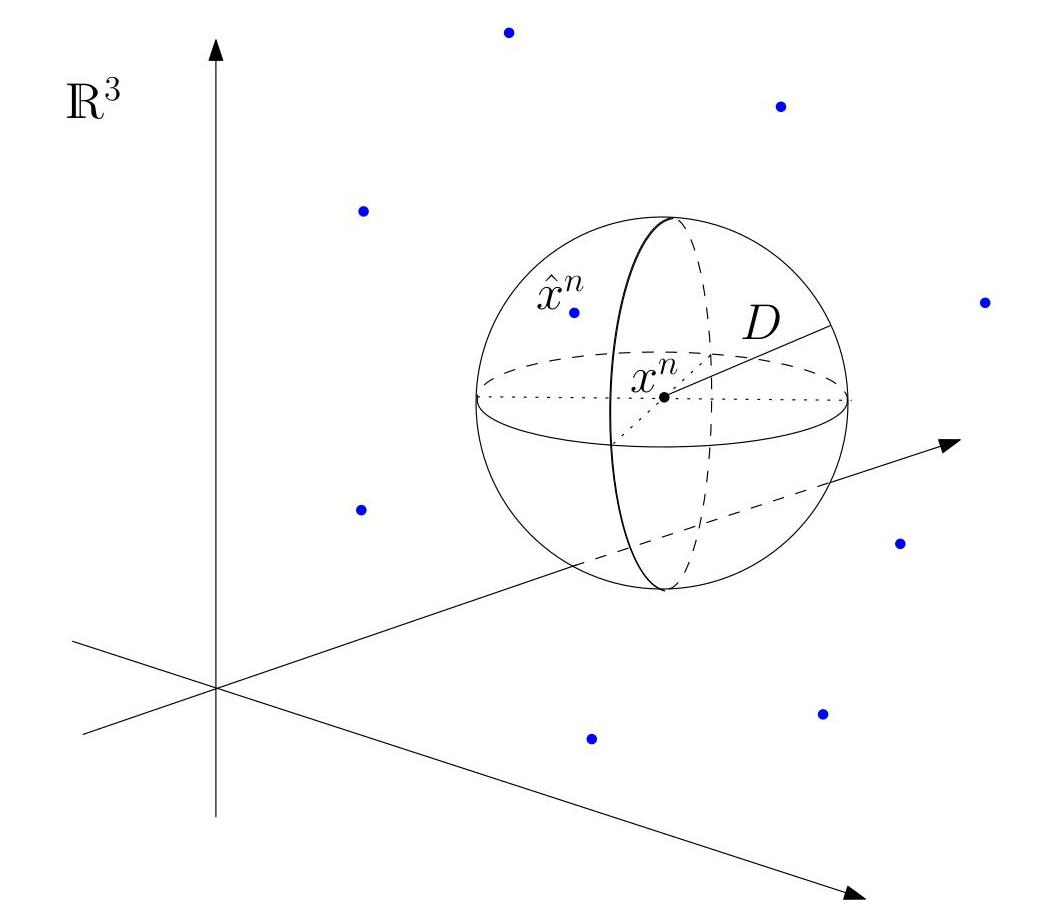
\includegraphics[scale=0.23]{img/sphere.jpg}
    \caption{Rappresentazione tridimensionale della regione di quantizzazione.}
    \label{fig:sphere}
\end{figure}
L'operazione di \textbf{quantizzazione} \`e data da una certa funzione $Q(\cdot)$
\begin{equation}
    \hat{x}_i = Q(x), \hspace{15pt} \text{se } x_i \leq x \leq x_{i+1}
\end{equation}
L'MSE \`e dato invece da
\begin{equation}
    D = \mathbb{E}[(x - Q(x))^2] =  \int_{-\infty}^{\infty} \Big ( x - Q(x) \Big )^2 f_X(x) dx = \sum_{i=1}^m \int_{x_i}^{x_{i+1}} (x - \hat{x}_i) f_X(x) dx
\end{equation}
La differenza tra il campione originario e quello quantizzato prende il nome di \textit{distorsione di quantizzazione} o \textit{rumore di quantizzazione}.

Ciascuno di questi intervalli dovr\`a essere poi codificato: se si usano per la codifica parole di codice della stessa lunghezza $l$ ($l = \lceil \log m \rceil$) la progettazione del quantizzatore, dati $f_X(x)$ e $m$, si riduce a determinare gli intervalli $x_i$ e i valori $\hat{x}_i$ che li rappresentano. Si potrebbero tuttavia utilizzare parole di lunghezza diversa $l_i$ (come ad esempio nella codifica di Huffman) e allora la scelta degli intervalli \textit{influenza anche il rate $R$ della sorgente}:
\begin{equation}
    R = \sum_{i=1}^m l_i p(\hat{x}_i) = \sum_{i=1}^m l_i \int_{x_i}^{x_{i+1}} f_X(x) dx
\end{equation}
Possiamo concludere che:
\begin{itemize}
    \item La distorsione $D$ dipende da come vengono scelti gli intervalli e dai \textit{valori} $\hat{x}_i$ scelti per rappresentarli.
    \item Il rate $R$ dipende da come vengono scelti gli intervalli e dai \textit{codici} usati per rappresentarli.
\end{itemize}
Si ha quindi che i problemi di trovare le migliori partizioni, rappresentazioni e codifica sono legati tra loro. \\
Quindi, ricapitolando: \\
Dato un limite di distorsione $D^*$ (massimo tollerato) si devono determinare gli intervalli di quantizzazione $[x_i, x_{i+1})$ e i valori che li rappresentano $\hat{x}_i$ in modo che soddisfino:
\begin{equation}
    \begin{cases}
    D \leq D^* \\
    R = \sum_{i} l_i p(\hat{x}_i) = \sum_i l_i \int_{x_i}^{x_{i+1}} f_X(x) dx
    \end{cases}
\end{equation}
oppure, equivalentemente, dato un limite massimo di rate $R^*$ si devono trovare i valori degli intervalli di quantizzazione $[x_i, x_{i+1})$ e le parole di codice tali che soddisfino:
\begin{equation}
    \begin{cases}
    R \leq R^* \\
    D = \int_{-\infty}^{\infty} \Big ( x - Q(x) \Big )^2 f_X(x) dx = \sum_{i}^m \int_{x_i}^{x_{i+1}} (x - \hat{x}_i) f_X(x) dx
    \end{cases}
\end{equation}
\subsubsection{Quantizzazione scalare}
Un quantizzatore scalare, associa ad ogni valore continuo della sorgente un valore $\hat{x}_i$ appartenente ad un set discreto di $m$ valori ciascuno dei quali rappresenta una particolare porzione dell’asse dei numeri reali $[x_i, x_{i+1})$ e $\hat{x}_i$ \`e un valore interno a tale intervallo. Un quantizzatore di largo impiego è quello \textbf{uniforme}, in cui tutti gli intervalli di
quantizzazione sono uguali. È completamente caratterizzato dall'ampiezza $\Delta$ dell'intervallo di quantizzazione (lo step di quantizzazione) e dal numero di livelli $m=2^R$.\\
Se la sorgente $X$ \`e uniforme sull'intervallo $[-A, A]$ si pu\`o pensare che la quantizzazione uniforme sia la scelta pi\`u appropriata: fissato $m$ vogliamo trovare il valore $\Delta$ che minimizza la distorsione $D$, ovvero l'errore di quantizzazione. Essendo la distribuzione uniforme si vede facilmente che 
\begin{equation}
    \Delta = \frac{2A}{m}
\end{equation}
e che l'errore di quantizzazione $e_q \coloneqq |x_i - \hat{x}_i|$ \`e distribuito uniformemente sull intervallo $[-\frac{\Delta}{2}, \frac{\Delta}{2}]$. La distorsione (MSE) in questo modo diventa
\begin{align*}
    D &= \mathbb{E} [ (X - \hat{X})^2] = \int_{-\infty}^{\infty} \Big ( x - Q(x) \Big )^2 f_X(x)dx = \\
    &= \sum_{i=1}^m \int_{x_i}^{x_{i+1}} (x - \hat{x}_i)^2 f_X(x) dx = \\
    &= \sum_{i=1}^m \frac{1}{2A} \int_{x_i}^{x_{i+1}} (x - \hat{x}_i)^2 dx = \frac{m}{2A} \int_{-\frac{\Delta}{2}}^{\frac{\Delta}{2}} x^2 dx = \\
    &= \frac{1}{\Delta} \int_{-\frac{\Delta}{2}}^{\frac{\Delta}{2}} x^2 dx = \frac{\Delta^2}{12}
\end{align*}
Ricordando che la varianza di una sorgente uniformemente distribuita su $[-A, A]$ \`e data da $A^2/3$ si ha che
\begin{equation}
    SNR = \frac{A^2/3}{\Delta^2/12} = \frac{12A^2}{3\Delta^2} = \frac{4A^2}{\Delta^2} = m^2 = 2^{2R} \approx 6R \hspace{2pt} db
\end{equation}

Non sempre la quantizzazione uniforme da buoni risultati, infatti l’errore di quantizzazione che si compie
dipende anche dalla statistica della sorgente. Il quantizzatore uniforme si comporta in maniera ottima
(minima potenza del rumore di quantizzazione) \textit{solo se le ampiezze dei campioni del segnale sono caratterizzate da una distribuzione uniforme}. Se la sorgente non è uniformemente distribuita ci sono range di valori in cui è più probabile avere un campione della sorgente ed è quindi meglio aumentare la densità dei livelli di quantizzazione nelle zone più popolate, in modo da avere una maggiore «accuratezza» dove si hanno più campioni, diminuendo di conseguenza la distorsione.\\
Quest'ultima può essere quindi ridotta scegliendo gli intervalli di quantizzazione in funzione delle statistiche
di $X$ (tenendo conto della pdf della sorgente), il che ci porta a una \textbf{quantizzazione non uniforme}: \textit{assegnare intervalli più stretti per le ampiezze più frequenti e intervalli di dimensioni crescenti per le ampiezze meno frequenti.} Facendo così si presta quindi più attenzione nella quantizzazione di valori che si presentano con maggiore probabilità diminuendo così l'errore di quantizzazione. \\
L'obiettivo della quantizzazione non uniforme è quindi trovare l’ampiezza degli intervalli ed i valori che li rappresentano tali che minimizzino la distorsione, fissato $m$.

\begin{figure}[H]
    \centering
    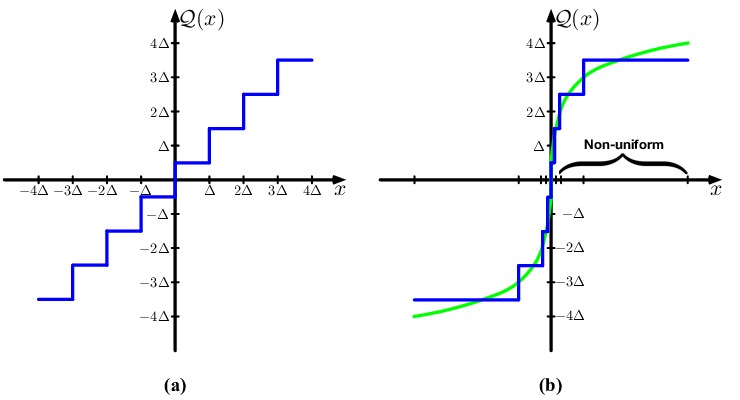
\includegraphics[scale=0.3]{img/uniform.png}
    \caption{Quantizzazione uniforme e quantizzazione non uniforme a confronto.}
    \label{fig:unif}
\end{figure}

\subsubsection{Quantizzazione vettoriale}
Il metodo più generale di quantizzazione è la \textbf{quantizzazione vettoriale}. Abbiamo già visto per la codifica lossless che codificare sequenze di simboli è più efficiente che codificare simboli isolati, nel caso della quantizzazione vettoriale si ha una sorta di dualit\`a rispetto a questo fatto: cos\`i come la quantizzazione scalare prevede una quantizzazione separata campione per campione quella vettoriale si occupa di quantizzare blocchi di campioni. Quest'ultima può portare ad una distorsione ben più bassa rispetto a quella scalare ed è ancora più efficiente se i campioni sono statisticamente \textit{dipendenti}.\\
Se $n$ \`e la cardinalit\`a del blocco emesso dalla sorgente (la lunghezza del messaggio) si ha che i livelli di quantizzazione sono vettori $\hat{x}_1^n, \hat{x}_2^n, \dots, \hat{x}_m^n \in \mathbb{R}^n$ con $m = 2^{nR}$. \\
La quantizzazione scalare quantizza ogni singolo simbolo separatamente in un livello mentre quella vettoriale vede l’intero vettore come un simbolo unico e lo quantizza in un unico livello.\\
Nella quantizzazione vettoriale si classificano blocchi di dati in un numero discreto di categorie (celle) in modo da ottimizzare qualche criterio (ad esempio la distorsione quadratica media): Le celle sono le “regioni di quantizzazione”, ovvero tutti i vettori in ingresso che cadono all’interno di una data cella sono associati alla stessa parola di codice. Il problema è definire le celle e i vettori di quantizzazione ad esse associate per poter effettuare questa sorta di \textit{pattern recognition}. Anche in questo caso si possono trovare dei metodi per definire le regioni di quantizzazione in relazione alla distribuzione di probabilità della sorgente (non uniforme).

\begin{minipage}{0.4\textwidth}
Se, ad esempio, avessimo $\mathbf{x} = (x_1, x_2)$ con $x_1, x_2 \in X$ si avrebbe $Q(\mathbf{x}) = (\hat{x}_1, \hat{x}_2) \in \mathbb{R}^2$ in cui i simboli $x_1, x_2$ verrebbero mappati sugli assi, inducendo una struttura a reticolo. Ad ogni cella viene associato un codice e l'unico grado di libert\`a \`e il livello di quantizzazione, lavorando in $\mathbb{R}$.
\begin{figure}[H]
    \centering
    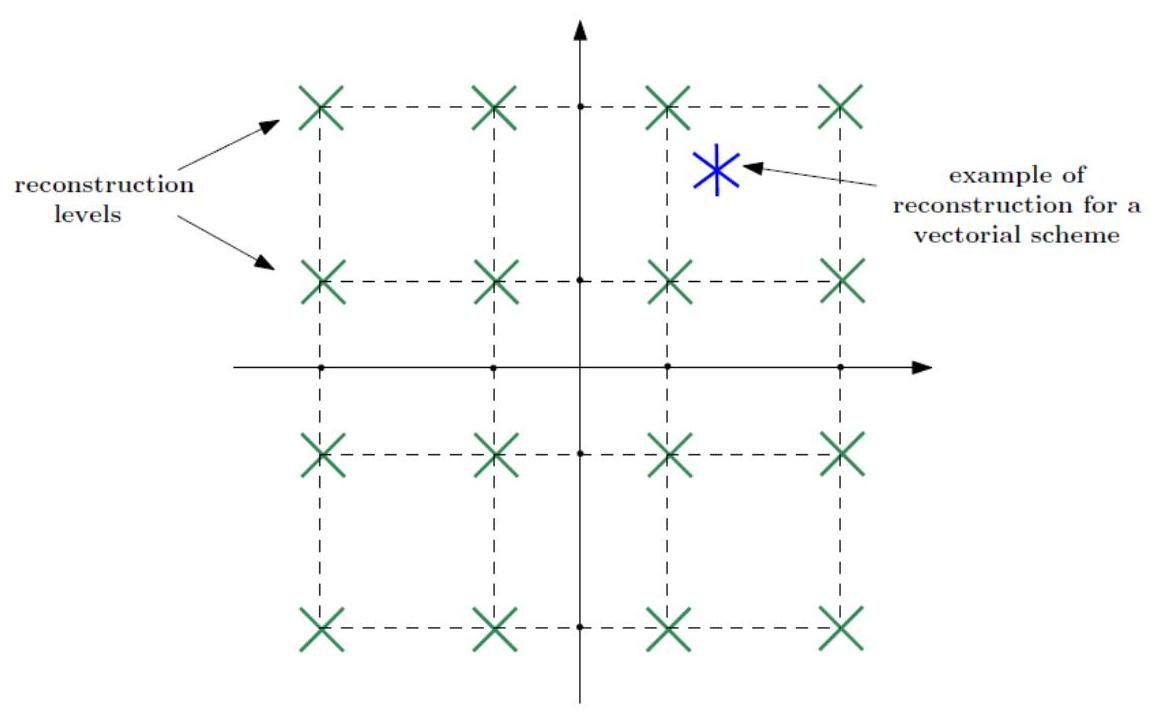
\includegraphics[scale=0.20]{img/ret.jpg}
    \caption{Quantizzazione a quadrati.}
    \label{fig:ret}
\end{figure}
\end{minipage} \hfill
\begin{minipage}{0.4\textwidth}
Con la quantizzazione vettoriale ci si svincola dalla forma quadrata delle celle: in questo caso, lavorando \textit{direttamente} in $\mathbb{R}^2$, il vettore quantizzato pu\`o assumere qualsiasi valore.
\begin{figure}[H]
    \centering
    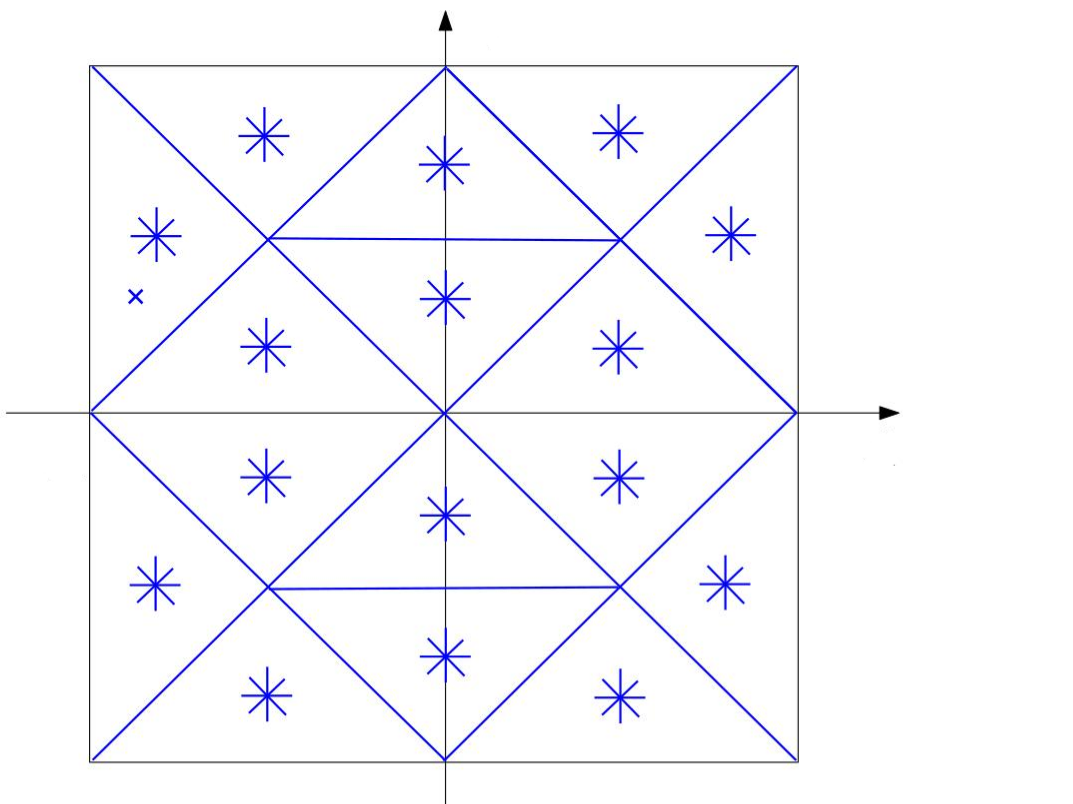
\includegraphics[scale=0.180]{img/vect.png}
    \caption{Tassellazione triangolare (esempio di quantizzazione vettoriale).}
    \label{fig:vect}
\end{figure}
\end{minipage} \\

Nella quantizzazione vettoriale c'\`e più libertà nella definizione delle regioni di quantizzazione perchè non si è vincolati ad una griglia rigida, come nel caso scalare. Anche nel caso di distribuzione uniforme con la quantizzazione vettoriale si riduce la distorsione. Si pu\`o mostrare che utilizzando, ad esempio, regioni esagonali
\begin{figure}[H]
    \centering
    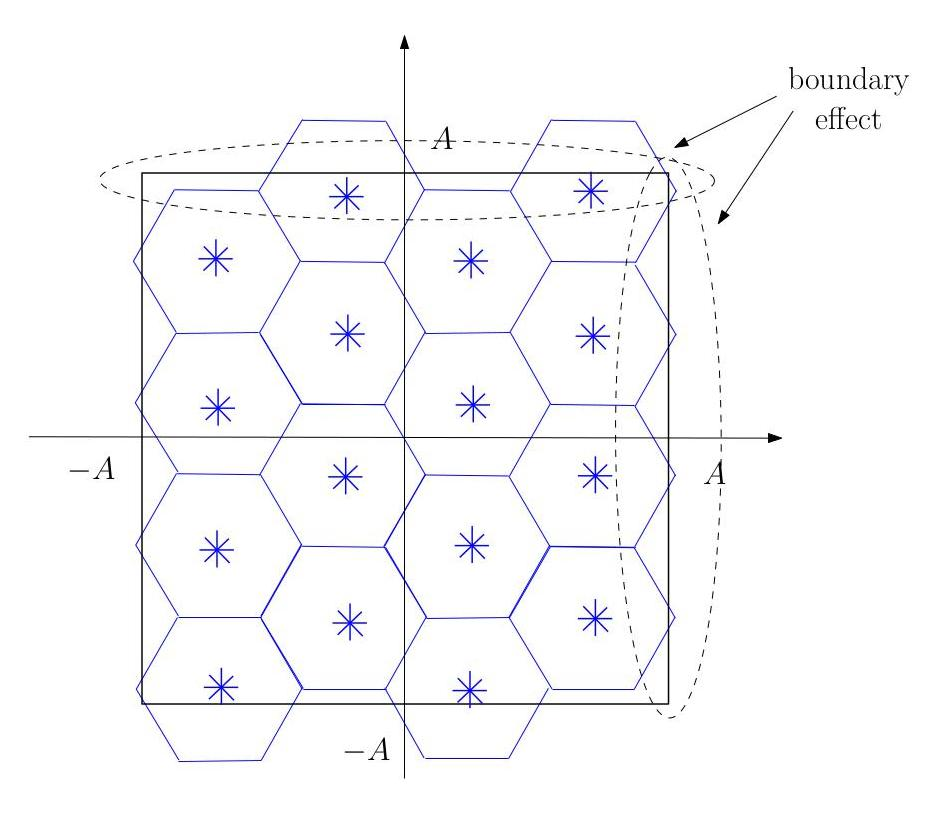
\includegraphics[scale=0.2]{img/hex.jpg}
    \caption{Tassellazione esagonale del dominio uniforme $[-A, A]^2$.}
    \label{fig:my_label}
\end{figure}
si pu\`o ridurre la distorsione. A parit\`a di area il calcolo dei momenti centrali d'inerzia suggerisce di utilizzare figure con pi\`u lati possibili, dovendoci avvicinare al minimo teorico dato dalla sfera. Questo induce per\`o dei problemi legati ad effetti di bordo, dati dal fatto che non \`e possibile ricoprire una regione quadrata con poligoni con pi\`u di 4 lati. Questo effetto diventa trascurabile all'aumentare del numero di intervalli di quantizzazione, ovvero eseguendo una \textit{quantizzazione fine}. 

\begin{mybox}{green}{\textit{\textbf{Esempio 2} : \textbf{Sorgenti con memoria. }}}
Nelle sorgenti con memoria, il beneficio è ancora più evidente: siano $X,Y$ due v.a. con pdf congiunta
\begin{equation}
    f_{XY}(x,y) = \begin{cases}
    \frac{1}{ab}, & (x,y) \in \mathcal{A}, \\
    0, & \text{ altrimenti.}
    \end{cases}
\end{equation}
dove $\mathcal{A}$ \`e la regione rettangolare delimitata da due lati $a$ e $b$ come in Figura \ref{fig:rett}:
\begin{figure}[H]
    \centering
    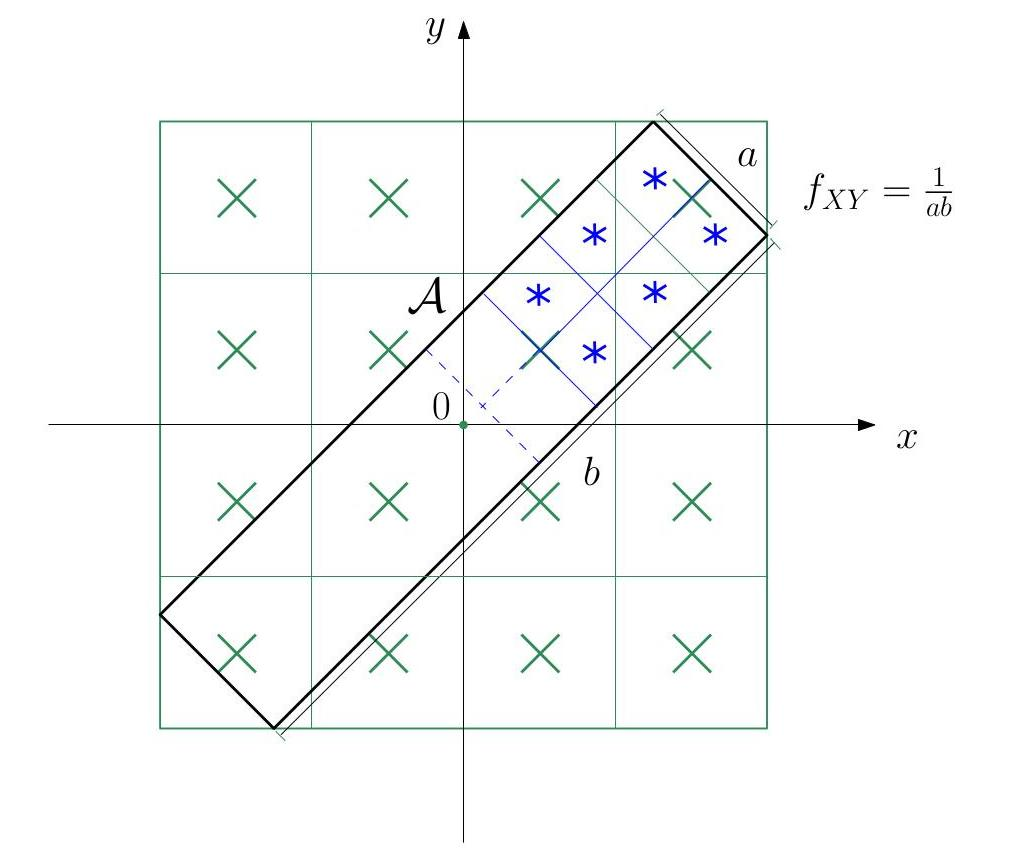
\includegraphics[scale=0.2]{img/rettang.jpg}
    \caption{Esempio di due v.a. correlate $X$ e $Y$. La quantizzazione vettoriale (stelline in blu) risulta necessaria dal momento che ogni struttura scalare (tassellazione in verde) porta ad una distribuzione non soddisfacente dei punti ricostruiti.}
    \label{fig:rett}
\end{figure}
Con la quantizzazione scalare si ottiene un risultato inefficiente dal momento che ci sono molte aree che non sono mai interessate dai valori, visto che questa tiene conto solo delle marginali $f_X(x), f_Y(y)$, non rendendo la quantizzazione efficiente dal punto di vista dello spreco di risorse. La correlazione tra $X$ e $Y$ rende necessario il dover ricorrere ad una quantizzazione vettoriale.
\end{mybox}

\newpage
\section{Capacit\`a di Canale} \label{sec:can}
Si considera ora il caso di una trasmissione in cui sia presente un canale non ideale, ovvero in cui \textit{non è certo che quello che viene inviato corrisponda a quello che viene ricevuto}. Il problema che ci poniamo è quindi l’\textbf{affidabilità} della trasmissione: la codifica di canale affronta il problema di trasmettere in maniera affidabile su un canale non affidabile. La codifica di canale è strettamente collegata alla capacit\`a di canale, ovvero alla capacità del canale di “far passare” l’informazione, che, come vedremo, ci porter\`a al Secondo Teorema di Shannon. Codifica di canale e di sorgente sono duali ma separate:
\begin{itemize}
    \item Con la codifica di sorgente si toglie la ridondanza per comprimere l’informazione.
    \item Con la codifica di canale si vuole aumentare l’affidabilità della trasmissione aggiungendo ridondanza al segnale trasmesso: si cerca un compromesso tra affidabilità ed efficienza realizzando un processo di codifica a controllo d’errore per ridurre gli effetti del rumore presente sul canale.
\end{itemize}
\subsection{Canale}
Il concetto di canale è piuttosto ampio: rappresenta ciò che succede ad un’informazione tra sorgente e
destinatario. Può includere, a seconda delle necessità, solo il mezzo fisico (ad esempio il solo doppino telefonico o un nastro magnetico) o, ad esempio, anche tutto ciò che è compreso tra un microfono e un altoparlante. Alcuni esempi di canale possono essere
\begin{itemize}
    \item Linea telefonica /ADSL (rumore termico, distorsioni, cross-talk, ...).
    \item Comunicazioni wireless (attenuazione atmosfera, rumore termico, interferenze, ...).
    \item Hard-disk\footnote{Non necessariamente la comunicazione deve avvenire tra due oggetti distinti, si pu\`o pensare che la sorgente e il destinatario siano lo stesso oggetto ma a tempi differenti, come nel caso della memorizzazione dell'informazione.} (errori di lettura/scrittura, materiali imperfetti, ...).
\end{itemize}
In ogni caso, in un canale, esiste \textit{sempre} la presenza di rumore che compromette la trasmissione.
\subsubsection{Canale discreto senza memoria}
\defn{\textit{Canale discreto senza memoria tempo-invariante:}} Si definisce canale discreto senza memoria tempo-invariante un canale in cui:
\begin{itemize}
    \item I simboli in uscita dalla sorgente (quindi in ingresso al canale) e in uscita dal canale, appartengano ad un alfabeto finito.
    \item In uscita dal canale si ha una sequenza che è casuale ma ha una distribuzione statistica che dipende dalla sequenza in ingresso.
    \item L’uscita in un determinato istante dipende solo dal simbolo in ingresso al canale in quell’istante e non
dai simboli precedentemente trasmessi.
    \item Le proprietà del canale non variano nel tempo.
\end{itemize}
Un canale discreto senza memoria tempo-invariante è univocamente definito dall’alfabeto di ingresso $A$, l'alfabeto di uscita $B$ e le \textit{forward probability} $p(b|a)$.
\begin{figure}[H]
    \centering
    
\includegraphics[width=\textwidth]{img/canale.jpg}
    \caption{Schema ad alto livello di un canale di comunicazione.}
    \label{fig:canale}
\end{figure}
In ricezione, dalla sequenza in uscita, si prova a ricostruire la sequenza di ingresso. Siccome per\`o due o più
input possono portare alla stessa parola in uscita dal canale, la ricostruzione della sequenza originaria può
essere \textbf{affetta da errori}: la comunicazione ha successo quando il ricevitore ed il trasmettitore \textit{concordano} su ciò che è stato trasmesso. Un canale può essere rappresentato con un grafo o, equivalentemente, con una matrice di canale $\mathcal{P}$

\begin{mybox}{green}{\textit{\textbf{Esempio 1} : \textbf{Rappresentazioni di canale}}}
Detto $X=\{x_1, x_2\}$ l'alfabeto d'ingresso e $Y = \{y_1, y_2, y_3\}$ l'alfabeto di uscita si hanno le seguenti rappresentazioni equivalenti

\begin{minipage}{0.45\textwidth}
\begin{figure}[H]
    \centering
    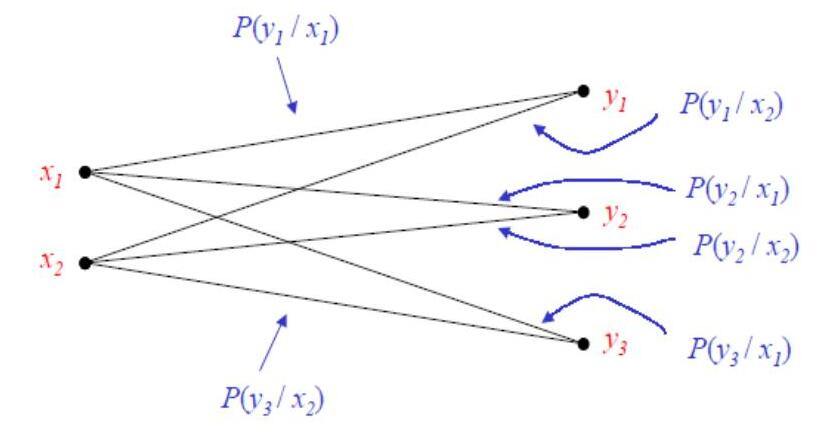
\includegraphics[scale=0.2]{img/grafo.jpg}
    \caption{Rappresentazione a grafo di un canale.}
\end{figure}
\end{minipage}
\begin{minipage}{0.45\textwidth}
\begin{equation*}
    \mathcal{P} = \begin{bmatrix}
    p(y_1|x_1) & p(y_2|x_1) & p(y_3|x_1) \\
    p(y_1|x_2) & p(y_2|x_2) & p(y_3|x_2) \\
    \end{bmatrix}
\end{equation*}
\end{minipage}
\end{mybox}
in cui si ha che le $\mathcal{P}_{ij} = p(b_j|a_i)$ e che le righe sommano ad $1$\footnote{Questo serve a garantire che per ogni input $a$ verr\`a effettivamente generato un output.}: $\sum_{j=1}^s p(b_j|a_i) = 1, \forall i=1,\dots,r$. \\
Se in ingresso al canale invece dei singoli elementi dell’alfabeto abbiamo sequenze di $n$ simboli dobbiamo fare riferimento all'estensione $n$-esima della sorgente $A^n$ e del destinatario $B^n$. Il canale in questo caso \`e completamente definito dai due alfabeti $A^n, B^n$ e dalla matrice di canale $\Pi$ data dal prodotto di Kronecker $n$ volte della matrice $\mathcal{P}$ del canale originario:
\begin{equation}
    \Pi = \underbrace{\mathcal{P} \otimes \mathcal{P} \otimes \dots \otimes \mathcal{P}}_n
\end{equation}
\\
Chiariamo la \textbf{notazione}:
\begin{itemize}
    \item $p(a)$ rappresenta la probabilit\`a \textbf{a priori} dei simboli in ingresso, ovvero la probabilit\`a che la sorgente emetta il simbolo $a$.
    \item $p(b)$ rappresenta la probabilità che a destinazione venga ricevuto il simbolo $b$.
    \item $p(a,b)$ rappresenta la probabilità congiunta che sia stato trasmesso il simbolo $a$ e che venga ricevuto il simbolo $b$.
    \item $p(b|a)$ rappresenta la probabilità condizionata che sia stato ricevuto il simbolo $b$ dato che è stato trasmesso il simbolo $a$, \`e quella che abbiamo definito \textbf{forward probability}.
    \item $p(a|b)$ rappresenta la probabilità condizionata che sia stato trasmesso il simbolo $a$ dato che è stato ricevuto il simbolo $b$, prende il nome di \textbf{backward probability}, ed \`e la probabilit\`a \textbf{a posteriori} dei simboli in ingresso.
\end{itemize}
Si possono quindi definire due entropie: l'entropia \textit{a priori}
\begin{equation}
    H(A) = \sum_{a \in A} p(a) \log \info{a}
\end{equation}
e l'entropia \textit{a posteriori}
\begin{equation}
    H(A|b) = \sum_{a \in A} p(a,b) \log \frac{1}{p(a|b)}
\end{equation}
che, come abbiamo detto, rappresentano il numero medio di cifre binarie necessarie per rappresentare $A$, rispettivamente considerando solo la sorgente e considerando di poter osservare la particolare uscita $b$ del canale. \\
Mediando su tutti i possibili simboli ricevuti
\begin{equation}
    H(A|B) = \sum_{b \in B} H(A|b) = \sum_{b \in A} \sum_{a \in A} p(a,b) \log \frac{1}{p(a|b)}
\end{equation}
si ha l’informazione media sulla sorgente conoscendo
i simboli ricevuti, ovvero l’incertezza rimasta su $A$ dopo aver conosciuto $B$. Questa quantit\`a prende il nome di \textbf{equivocazione di canale} e rappresenta l’informazione aggiuntiva che serve in ricezione dopo aver osservato $B$, quindi \textbf{ci\`o che si \`e perso a causa del canale}.\\
Se ci mettiamo dalla parte del destinatario al tempo $0$ non abbiamo visto arrivare alcun simbolo dal
canale e la nostra “incertezza” sulla sorgente $A$ è pertanto l’entropia $H(A)$. Dopo l'osservazione però, la nostra incertezza si riduce a $H(A|B)$. L'informazione che ha viaggiato sul canale \`e dunque
\begin{equation}
    H(A) - H(A|B) = I(A;B) = \sum_{a \in A} \sum_{b \in B} p(a,b) \frac{p(a,b)}{p(a)p(b)}
\end{equation}
Infatti, ricordando che $I(A;B)$ è l’informazione contenuta sia in $A$ che in $B$, si ha che questa rappresenta ciò che effettivamente ha attraversato il canale. Di conseguenza la \textit{massima quantità di informazione che può viaggiare attraverso un canale è data dal massimo valore che può assumere l’informazione mutua}.

\subsubsection{Capacit\`a di Canale}
Abbiamo detto quindi che la massima quantità di informazione che può viaggiare attraverso un canale è quindi data dal massimo valore che può assumere l'informazione mutua. Questa per\`o dipende sia dalla probabilit\`a a priori $p(a)$ che dalla forward probability $p(b|a)$ quindi, rispettivamente, dalla sorgente e dalla matrice di canale. Infatti quanta informazione arriva a destinazione dipende sia dal tipo di canale considerato che anche dall’uso che viene fatto del canale. Se vogliamo massimizzare l’informazione trasportata dal canale dobbiamo anche agire sulla sorgente. \\
Al fine di caratterizzare un canale discreto senza memoria \textbf{indipendentemente dalla sorgente in ingresso}, si definisce capacità del canale il valore massimo dell’informazione mutua rispetto a tutte le possibili distribuzioni delle probabilità dei simboli di ingresso:
\defn{\textit{Capacit\`a di Canale:}} Misurata in $[bit/simbolo]$ la capacit\`a di canale $\mathcal{C}$ \`e  definita come
\begin{equation}
    \mathcal{C} \coloneqq \max_{p(a)} I(A;B)
\end{equation}
Se si massimizza su $p(a)$, $\mathcal{C}$ dipende solo dal canale stesso e \textit{rappresenta il massimo flusso informativo che può essere sopportato dal canale}. Se, inoltre, la sorgente genera simboli con una frequenza $f$ ($[simboli/s]$) la capacit\`a di canale per unit\`a di tempo \`e data da
\begin{equation}
    \mathcal{C}_t \coloneqq f \mathcal{C}, \hspace{15pt} [bit/s]
\end{equation}
La capacità di canale per unità di tempo $\mathcal{C}_t$ rappresenta la \textit{massima velocità di trasferimento dell’informazione permessa dal canale}. Si hanno alcune propriet\`a per la capacit\` di canale:
\begin{itemize}
    \item $\mathcal{C} \geq 0$
    \item $\mathcal{C} \leq \log |A|$ (dato che $I(A;B) \leq H(A) \leq \log |A|$)
    \item $\mathcal{C} \leq \log |B|$ (dato che $I(A;B) \leq H(B) \leq \log |B|$)
    \item $I(A;B)$ \`e una funzione continua di $p(a)$
    \item $I(A;B)$ \`e una funzione concava di $p(a)$, per cui si ha coincidenza tra massimi locali e massimi globali.
\end{itemize}
Per determinare la capacità si deve quindi effettuare una massimizzazione. Si possono quindi usare tecniche di ottimizzazione, anche se in generale non è semplice. Ci sono per\`o dei casi particolari in cui la capacità può essere calcolata senza troppi sforzi, vediamone alcuni.
\subsubsection{Canale senza rumore}
Un canale si definisce \textbf{senza rumore} (noiseless) se è caratterizzato da una matrice di canale $\mathcal{P}$ con $1$ solo elemento non
nullo in ogni colonna. In questo tipo di canale quindi il destinatario sa sempre che simbolo \`e stato inviato mentre il mittente non è in grado di sapere cosa il destinatario abbia ricevuto. Ricordando che $\mathcal{P}$ \`e data da
\begin{equation}
    \mathcal{P} = \begin{bmatrix}
    p(b_1|a_1) & p(b_2|a_1) & \dots & p(b_s|a_1) \\
    p(b_1|a_2) & p(b_2|a_2) & \dots & p(b_s|a_2) \\
    \vdots & \vdots & & \vdots \\
     p(b_1|a_r) & p(b_2|a_r) & \dots & p(b_s|a_r) \\
    \end{bmatrix}
\end{equation}
se un solo elemento per colonna $j$ \`e diverso da $0$ quel simbolo $b_j$ pu\`o essere ottenuto solo con un possibile $a_i$.
Se il canale è noiseless allora $H(A|B) = 0$, ovvero l’equivocazione di canale è nulla, e l'osservazione dell’uscita ci restituisce esattamente l’ingresso.
\begin{mybox}{green}{\textit{\textbf{Esempio 2} : \textbf{Canale senza rumore}}}
\begin{minipage}{0.45\textwidth}
\begin{figure}[H]
    \centering
    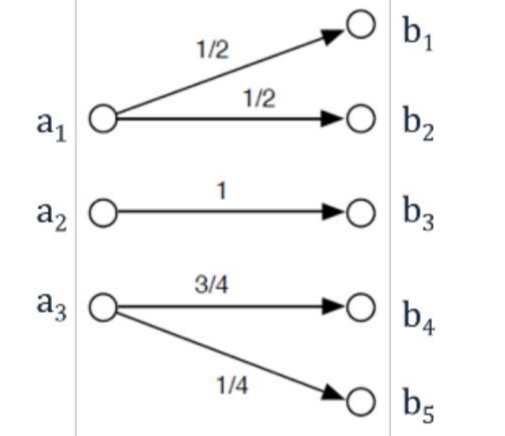
\includegraphics[scale=0.2]{img/detchan.png}
    \caption{Grafo di un canale senza rumore.}
\end{figure}
\end{minipage}
\begin{minipage}{0.45\textwidth}
\begin{equation*}
    \mathcal{P} = \begin{bmatrix}
    1/2 & 1/2 & 0 & 0 & 0 \\
    0 & 0 & 1 & 0 & 0 \\
    0 & 0 & 0 & 3/4 & 1/4
    \end{bmatrix}
\end{equation*}
\end{minipage}
\end{mybox}
Infatti, conoscendo $b$ si determina univocamente $a$ e la probabilit\`a a posteriori \`e data da
\begin{equation*}
    p(a|b) = 
    \begin{cases} 
    1, & \text{se \`e stato trasmesso } a \\
    0, & \text{altrimenti.}
    \end{cases}
\end{equation*}
da cui
\begin{equation*}
    H(A|B) = \sum_{a \in A} \sum_{b \in B} p(a,b) \log \frac{1}{p(a|b)} = 0
\end{equation*}
Si ha quindi che
\begin{equation*}
    I(A;B) = H(A) - H(A|B) = H(A) = \sum_{a \in A} p(a) \info{a}
\end{equation*}
e che, ricordando che l'entropia di una sorgente \`e massima quando i simboli sono tutti equiprobabili\footnote{Cio\`e $p(a) = 1/|A| = 1/r$.} vale 
\begin{equation}
    \mathcal{C} = \max_{p(a)} I(A;B) = \max_{p(a)} \sum_{a \in A} p(a) \info{a} = \log |A|
\end{equation}
\subsubsection{Canale deterministico}
Un canale si definisce \textbf{deterministico} se è caratterizzato da una matrice di canale $\mathcal{P}$ con un solo elemento
unitario in ogni riga. \textit{Il mittente sa sempre che simbolo viene ricevuto mentre il destinatario non sa ci\`o che \`e stato inviato}.
\begin{mybox}{green}{\textit{\textbf{Esempio 3} : \textbf{Canale deterministico}}}
\begin{minipage}{0.45\textwidth}
\begin{figure}[H]
    \centering
    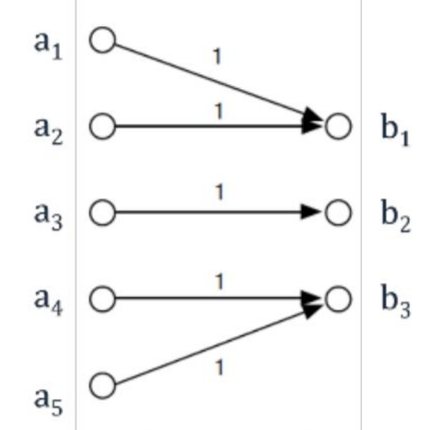
\includegraphics[scale=0.2]{img/determ.png}
    \caption{Grafo di un canale deterministico.}
\end{figure}
\end{minipage}
\begin{minipage}{0.45\textwidth}
\begin{equation*}
    \mathcal{P} = \begin{bmatrix}
    1 & 0 & 0 \\
    1 & 0 & 0 \\
    0 & 1 & 0 \\
    0 & 0 & 1 \\
    0 & 0 & 1 \\
    \end{bmatrix}
\end{equation*}
\end{minipage}
\end{mybox}
Se un solo elemento per riga $i$ \`e uguale a $1$ allora quel valore $a_i$ pu\`o essere ottenuto solo con un possibile $b_j$. Nel canale deterministico infatti conoscere l’ingresso vuol dire conoscere l’uscita, il che implica $H(B|A) = 0$. Poich\`e quindi l’incertezza che rimane su $B$ conoscendo $A$ è nulla si ha 
\begin{equation*}
    I(A;B) = I(B;A) = H(B) - H(B|A) = H(B) = \sum_{b \in B} p(b) \log \info{b}
\end{equation*}
da cui, similmente al caso precedente
\begin{equation}
    \mathcal{C} = \max_{p(a)} I(A;B) = \max_{p(a)} \sum_{b \in B} p(b) \info{b} = \log |B|
\end{equation}
In questo caso, infine, l’equivocazione di canale è data da $H(A|B) = H(A) - H(B)$.

\subsubsection{Canale completamente ceterministico}
Un canale si dice \textbf{completamente deterministico} (corrispondenza uno ad uno) se è sia noiseless che deterministico. In questo caso quindi sia il mittente che il destinatario sanno cosa \`e stato ricevuto/inviato. Alfabeto di ingresso e di uscita
hanno quindi la stessa dimensione, dovendo essere il canale biettivo.
\begin{mybox}{green}{\textit{\textbf{Esempio 4} : \textbf{Canale completamente deterministico}}}
\begin{minipage}{0.45\textwidth}
\begin{figure}[H]
    \centering
    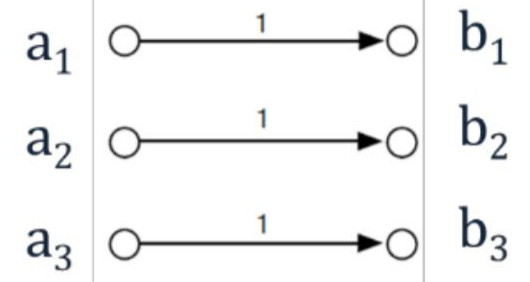
\includegraphics[scale=0.2]{img/cdet.png}
    \caption{Grafo di un canale completamente deterministico.}
\end{figure}
\end{minipage}
\begin{minipage}{0.45\textwidth}
\begin{equation*}
    \mathcal{P} = \begin{bmatrix}
    1 & 0 & 0 \\
    0 & 1 & 0 \\
    0 & 0 & 1 \\
    \end{bmatrix}
\end{equation*}
\end{minipage}
\end{mybox}
Si ha quindi $I(A;B) = H(A) = H(B)$ da cui 
\begin{equation}
    \mathcal{C} = \log r = \log s
\end{equation}

\subsubsection{Canale inutile}
Un canale di definisce \textbf{inutile} se le uscite sono indipendenti dagli ingressi: $p(b|a) = p(b)$. Il destinatario non può derivare alcuna informazione dalla comunicazione, che è stata appunto inutile. Le colonne sono composte da elementi uguali, per cui tutte le righe sono identiche. L'uscita non dipende quindi dall'ingresso.
\begin{mybox}{green}{\textit{\textbf{Esempio 5} : \textbf{Canale inutile}}}
\begin{minipage}{0.45\textwidth}
\begin{figure}[H]
    \centering
    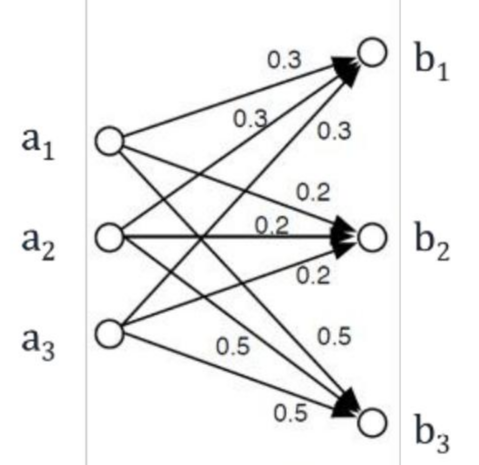
\includegraphics[scale=0.2]{img/inutile.png}
    \caption{Grafo di un canale inutile.}
\end{figure}
\end{minipage}
\begin{minipage}{0.45\textwidth}
\begin{equation*}
    \mathcal{P} = \begin{bmatrix}
    0.3 & 0.2 & 0.5 \\
    0.3 & 0.2 & 0.5 \\
    0.3 & 0.2 & 0.5    
    \end{bmatrix}
\end{equation*}
\end{minipage}
\end{mybox}
Si ha quindi che
\begin{align*}
    H(B|A) &= \sum_{b \in B} \sum_{a \in A} p(a,b) \info{b|a} = \sum_{b \in B} \sum_{a \in A} p(b|a) p(a) \info{b} = \\
    &= \underbrace{\sum_{a \in A} p(a)}_{=1} \sum_{b \in B} \underbrace{p(b|a)}_{=p(b)} \info{b} = \sum_{b \in B} p(b) \info{b} = H(B)
\end{align*}
da cui
\begin{equation*}
    I(A;B) = I(B;A) = H(B) - H(B|A) = H(B) - H(B) = 0
\end{equation*}
e quindi
\begin{equation}
    \mathcal{C} = \max_{p(a)} I(A;B) = 0
\end{equation}

\subsubsection{Canale simmetrico e Canale simmetrico binario}
Un canale di definisce \textbf{simmetrico} se la sua matrice di canale è caratterizzata da righe e colonne che sono
permutazioni degli stessi numeri. Ad esempio:
\begin{equation*}
    \mathcal{P} = \begin{bmatrix}
    0.3 & 0.2 & 0.5 \\
    0.2 & 0.5 & 0.3 \\
    0.5 & 0.3 & 0.2    
    \end{bmatrix}
\end{equation*}
In questo caso si ha che $H(B|A)$ \`e indipendente dalla sorgente ma dipende unicamente dalla matrice $\mathcal{P}$. Dal momento che ogni riga contiene gli stessi valori, indicando con $k$ una costante, si ha che vale
\begin{equation}
    \sum_{j=1}^s p(b_j|a_i) \info{b_j|a_i} = k
\end{equation}
rendendo questa quantit\`a invariante rispetto alla riga (valendo $\forall i = 1, \dots, r$). Si ha quindi che
\begin{align*}
    H(B|A) &= \sum_{b \in B} \sum_{a \in A} p(a,b) \info{b|a} = \sum_{b \in B} \sum_{a \in A} p(b|a)p(a) \info{b|a} = \\
    &= \sum_{a \in A} p(a) \underbrace{\sum_{b \in B} p(b|a) \info{b|a}}_{=k} = k \sum_{a \in A} p(a) = k
\end{align*}
da cui
\begin{equation*}
    I(A;B) = I(B;A) = H(B) - H(B|A) = H(B) - k
\end{equation*}
ovvero che l’informazione mutua dipende da sia da $H(B)$ che dalla matrice di canale e l’unico modo per avere la massima $I(A;B)$ è massimizzare $H(B)$, il che vuol dire avere simboli equiprobabili. \textit{In un canale simmetrico per\`o si hanno simboli in uscita equiprobabili se i simboli in ingresso sono equiprobabili}. Infatti se $p(a) = 1/r$ vale 
\begin{equation}
    p(b) = \sum_{a \in A} p(a,b) = \sum_{a \in A} p(b|a)p(a) = \frac{1}{r} \sum_{a \in A} p(b|a) = \frac{col}{r} = \frac{1}{s}
\end{equation}
dove $col$ rappresenta la somma degli elementi di una colonna della matrice (tutte le colonne sommano a $col$ per definizione).

\begin{mybox}[breakable]{green}{}
Prendiamo ad esempio un canale debolmente simmetrico (un canale si dice debolmente simmetrico quando ogni riga \`e una permutazione di ogni altra riga e le colonne sommano allo stesso valore $col$) di questo tipo
\begin{equation*}
    \mathcal{P} = \begin{bmatrix}
    1/3 & 1/6 & 1/2 \\
    1/3 & 1/2 & 1/6
    \end{bmatrix}
\end{equation*}
Se imponiamo $\forall a \in A$, $p(a) = 1/2$ si ha $p(b) = \frac{1}{2} \times \frac{2}{3} = \frac{1}{3}, \forall b \in B$.
\end{mybox}

In generale si ha quindi che la capacità di un canale simmetrico è
\begin{equation}
    \mathcal{C} = \log(s) - k
\end{equation}

Il \textbf{canale simmetrico binario} (BSC) è un particolare canale simmetrico composto da due simboli in ingresso e da due simboli in uscita $A = B = \{0,1\}$ in cui si ha che $p$ rappresenta la probabilità che ci sia un errore di trasmissione. Si ha quindi che $Pr\{B=1|A=0\} = p = Pr\{B=0|A=1\}$ e $Pr\{B=1|A=1\} = 1-p = Pr\{B=0|A=0\}$:

\begin{minipage}{0.45\textwidth}
\begin{figure}[H]
    \centering
    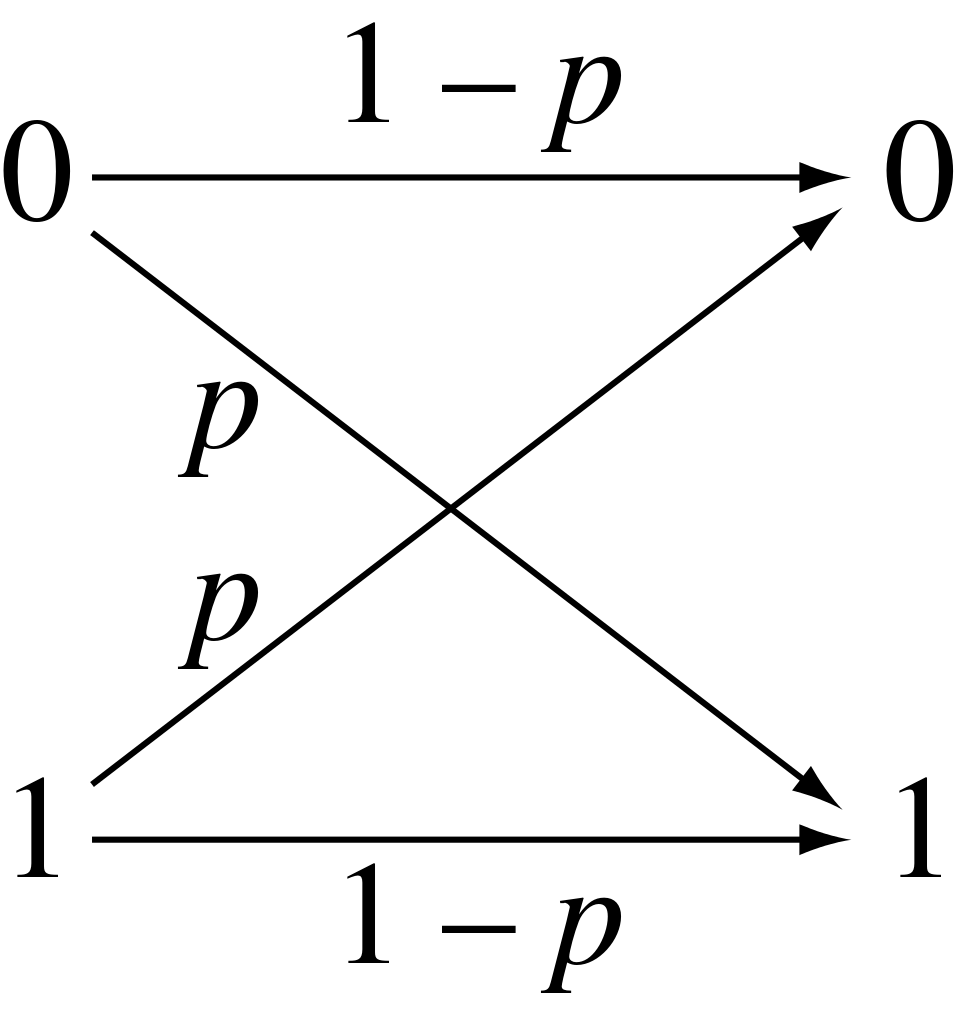
\includegraphics[scale=0.08]{img/bsc.png}
    \caption{Grafo di un canale simmetrico binario.}
\end{figure}
\end{minipage}
\begin{minipage}{0.45\textwidth}
\begin{equation*}
    \mathcal{P} = \begin{bmatrix}
    1-p & p \\
    p & 1-p \\
    \end{bmatrix}
\end{equation*}
\end{minipage}

Verifichiamo che una probabilit\`a uniforme in ingresso implica una probabilit\`a uniforme in uscita:
\begin{align*}
    Pr\{B=0\} &= Pr\{B=0|A=0\}Pr\{A=0\} + Pr\{B=0|A=1\}Pr\{A=1\} = \\
    &= (1-p)Pr\{A=0\} + pPr\{A=1\} \\
    Pr\{B=1\} &= Pr\{B=1|A=0\}Pr\{A=0\} + Pr\{B=1|A=1\}Pr\{A=1\} = \\
    &= pPr\{A=0\} + (1-p)Pr\{A=1\} \\
    \text{Quindi }Pr\{&A=0\} = Pr\{A=1\} = \frac{1}{2} \implies Pr\{B=0\} = Pr\{B=1\} = \frac{1}{2}
\end{align*}
Il BSC \`e il modello più semplice di canale con errori, tuttavia riesce a rappresentare bene la complessità del problema.
\begin{align*}
    I(A;B) &= H(B) - H(B|A) = H(B) - \sum_{a \in A}p(a) H(B|a) = \\
    & \overset{\rho}{=} H(B) - \sum_{a \in A} p(a) H(p) = H(B) - H(p) \leq 1 - H(p)
\end{align*}
Dove l'ultima disuguaglianza vale perch\`e $H(B) \leq 1$ e $H(p)$ \`e l'entropia di una sorgente binaria con probabilit\`a $p$:
\begin{equation*}
    H(p) = p \log \frac{1}{p} + (1-p) \log \frac{1}{1-p}
\end{equation*}
mentre l'uguaglianza $\rho$ vale perch\`e, chiamando 
\begin{itemize}
    \item $p(b_0) \coloneqq Pr\{B=0\}$
    \item $p(b_0|a_0) \coloneqq Pr\{B=0|A=0\} = 1-p $ 
    \item $p(a_1) \coloneqq Pr\{A=1\}$
    \item $\dots$
\end{itemize} si ha
\begin{align*}
&H(B|A) = \sum_{a \in A} \sum_{b \in B} p(b|a)p(a)\info{b|a} = p(b_0|a_0)p(a_0)\info{b_0|a_0} + \\
&+p(b_0|a_1)p(a_1)\info{b_0|a_1} + p(b_1|a_0)p(a_0)\info{b_1|a_0} + p(b_1|a_1)p(a_1)\info{b_1|a_1} = \\
&=p(a_0) \Big [p(b_0|a_0)\info{b_0|a_0} + p(b_1|a_0)\info{b_1|a_0} \Big ] + p(a_1) \Big [p(b_0|a_1)\info{b_0|a_1} + p(b_1|a_1)\info{b_1|a_1} \Big ] = \\
&=p(a_0) \Big [(1-p)\log \frac{1}{1-p} + p \log \frac{1}{p} \Big ] + p(a_1) \Big[ p \log \frac{1}{p} + (1-p)\log \frac{1}{1-p}  \Big ] = \\
& \Big [ p(a_0) + p(a_1) \Big ] \Big [ (1-p)\log \frac{1}{1-p} + p \log \frac{1}{p} \Big ] = H(p)
\end{align*}
Ricordando (vedi Fig. \ref{fig:binentropy}) che l'entropia di una sorgente binaria \`e massima quando la probabilit\`a \`e uniforme si ha
\begin{equation}
    \mathcal{C} = \max_{p(a)} I(A;B) = 1 - H(p)
\end{equation}
L'entropia di $B$ \`e massima quando $p(b)$ \`e uniforme, ma ci\`o vuol dire che la $p(a)$ deve essere uniforme. La capacit\`a di canale di un canale binario simmetrico \`e quindi massima quando la probabilit\`a a priori $p(a)$ \`e uniforme.

\subsubsection{Binary Erasure Channel}
Nel \textbf{binary erasure channel} il mittente può inviare due diversi simboli al destinatario. Un simbolo può essere ricevuto correttamente oppure pu\`o essere \textbf{perso} (in questo caso il destinatario riceve uno speciale simbolo \#). Il canale \`e caratterizzato dalla probabilit\`a $p$ che il simbolo venga perso:

\begin{minipage}{0.45\textwidth}
\begin{figure}[H]
    \centering
    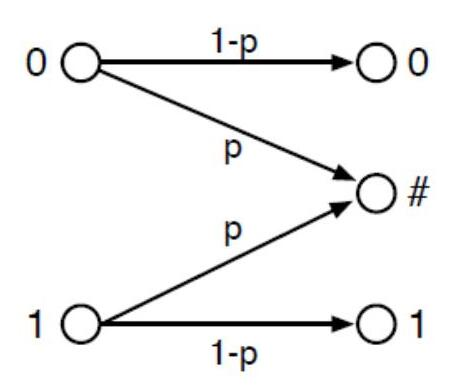
\includegraphics[scale=0.2]{img/erasure.jpg}
    \caption{Grafo di un BEC.}
\end{figure}
\end{minipage}
\begin{minipage}{0.45\textwidth}

\begin{equation*}
    \mathcal{P} = \overbrace{\begin{bmatrix}
    1-p & p & 0 \\
    0 & p & 1-p \\
    \end{bmatrix}}^{0 \hspace{20pt} \# \hspace{20pt} 1}
\end{equation*}
\end{minipage}

Se \`e stato trasmesso $0$ non si può ricevere $1$ e viceversa. Questo modello assume quindi che gli $0$ e $1$ ricevuti vengano ricevuti sempre correttamente e, viceversa, se si \`e ricevuto \# si ha un'ambiguit\`a sul simbolo trasmesso e questa ricezione viene scartata (da qu\`i il nome di BEC). Chiamando $Pr\{A=0\} \coloneqq w, Pr\{A=1\} =1-w$ e avendo che
\begin{itemize}
    \item $Pr\{B=0|A=0\} = Pr\{B=1|A=1\} = 1-p$
    \item $Pr\{B=\#|A=0\} = Pr\{B=\#|A=1\} = p$
    \item $Pr\{B=1|A=0\} = Pr\{B=0|A=1\} = 0$
\end{itemize}
calcoliamo $H(B)$ e $H(B|A)$. Si ha
\begin{align*}
    H(B) &= (1-p)w \log \frac{1}{(1-p)w} + (1-p)(1-w)\log \frac{1}{(1-p)(1-w)} + p \log \frac{1}{p} = \\
    &= (1-p) \Big [ w \log \frac{1}{(1-p)w} + (1-w)\log \frac{1}{(1-p)(1-w)} \Big] + p \log \frac{1}{p} = \\
    &=(1-p) \Big [ w \log \frac{1}{1-p} + w \log \frac{1}{w} + (1-w)\log \frac{1}{1-p} + (1-w)\log \frac{1}{1-w} \Big ] + p \log \frac{1}{p} = \\
    &=(1-p) \Big [ \log \frac{1}{1-p} + H(w) \Big] + p \log \frac{1}{p} =H(p) + (1-p)H(w)
\end{align*}.
\begin{align*}
    H(B|A) &= \sum_{a\in A} \sum_{b \in B} p(b|a)p(a) \log \frac{1}{p(b|a)} = \\
    &= w \Big [(1-p) \log \frac{1}{1-p} + p \log \frac{1}{p} + 0 \Big ] + (1-w) \Big [0 + p \log \frac{1}{p} + (1-p) \log \frac{1}{1-p} \Big ] = \\
    &= w H(p) + (1-w)H(p) = H(p)
\end{align*}
Quindi si ha
\begin{equation*}
    I(A;B) = H(B) - H(B|A) = H(p) + (1-p)H(w) - H(p) = (1-p)H(w)
\end{equation*}
da cui
\begin{equation}
    \mathcal{C} = \max_{p(a)} I(A;B) = \max_{w} (1-p)H(w) = 1-p
\end{equation}
\subsection{Canali in cascata}
\begin{figure}[H]
    \centering
    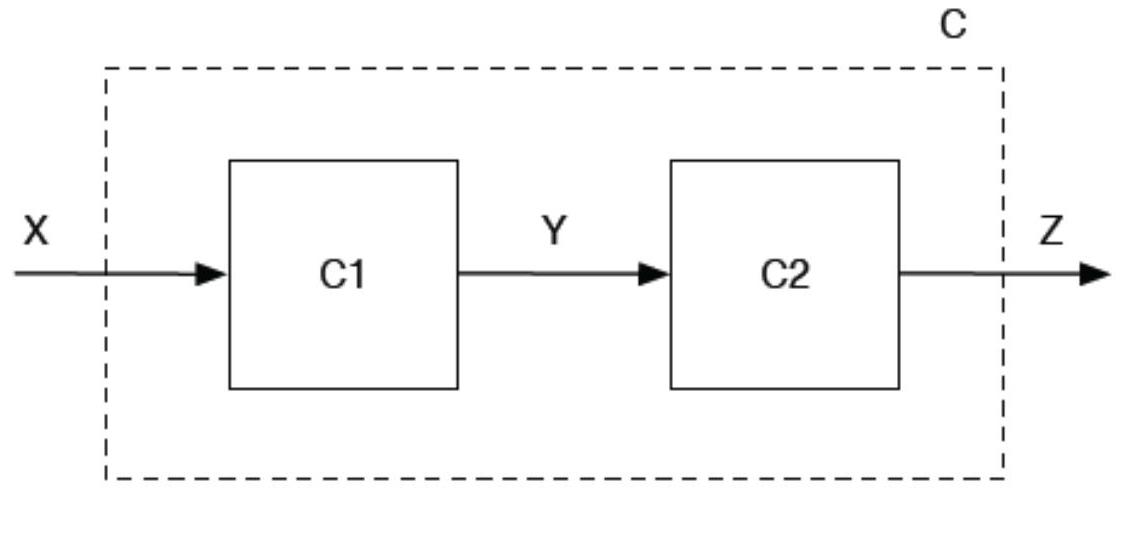
\includegraphics[scale=0.2]{img/cascata.jpg}
    \caption{Due canali in cascata $C_1$ e $C_2$.}
\end{figure}
Due canali $C_1$ e $C_2$ possono essere posti in \textit{cascata}, ovvero uno di seguito all'altro. La matrice di
canale che si ottiene ponendo in cascata due canali $C_1, C_2$ è il prodotto delle matrici di canale dei due canali, ovvero
\begin{equation}
    \mathcal{P}_c = \mathcal{P}_1 \mathcal{P}_2
\end{equation}
Si può verificare che per i canali in cascata l'informazione mutua, man mano che si attraversano i canali, non può aumentare: ad ogni passaggio si può \textbf{solo perdere} informazione e mai guadagnarne:
\begin{equation*}
    \begin{cases}
    H(X|Z) \geq H(X|Y) \implies I(X;Z) \leq I(X;Y)\\
    H(X|Z) \geq H(Y|Z) \implies I(X;Z) \leq I(Y;Z)
    \end{cases}
\end{equation*}
\begin{mybox}{green}{\textbf{\textit{Esempio 6: BSC in cascata}}}
Siano $C_1$ e $C_2$ due BSC in cascata con matrici di canale
\begin{equation*}
    \mathcal{P}_1 = \begin{bmatrix}
    1-p_1 & p_1 \\
    p_1 & 1-p_1
    \end{bmatrix}, \quad 
    \mathcal{P}_2 = \begin{bmatrix}
    1-p_2 & p_2 \\
    p_2 & 1-p_2
    \end{bmatrix}
\end{equation*}
Allora si ha che la matrice di canale risultante \`e data da
\begin{equation*}
    \mathcal{P}_c = \mathcal{P}_1 \mathcal{P}_2 = \begin{bmatrix}
    (1-p_1)(1-p_2) + p_1p_2 & (1-p_1)p_2 + (1-p_2)p_1 \\
    (1-p_1)p_2 + (1-p_2)p_1 & (1-p_1)(1-p_2) + p_1p_2
    \end{bmatrix}
\end{equation*}
da cui, se $p_1 = p_2 = p$ e $(1-p_1)=(1-p_2) = \bar{p}$ si ha
\begin{equation*}
    \mathcal{P}_c = \begin{bmatrix}
    p^2 + \bar{p}^2 & 2 p \bar{p} \\
    2 p \bar{p} & p^2 + \bar{p}^2
    \end{bmatrix}
\end{equation*}
Le due capacit\`a dei singoli tratti valgono quindi
\begin{equation*}
    \mathcal{C}_1 = \mathcal{C}_2 = 1 - H(p)
\end{equation*}
mentre la capacit\`a del canale in cascata \`e
\begin{equation*}
    \mathcal{C}_c = 1 - H(2p\bar{p}) \leq \mathcal{C}_1 = \mathcal{C}_2
\end{equation*}
\end{mybox}
\subsection{Probabilit\`a di Errore e Regola di Decisione}
Se il canale introduce rumore, $H(A|B) \neq 0$, ciò che arriva:
\begin{itemize}
    \item Può essere uguale a quello trasmesso con una certa probabilità.
    \item Può essere diverso da quello trasmesso con un’altra probabilità.
\end{itemize}
quindi il sistema è caratterizzato ovviamente da una certa probabilità di errore.

\textit{Il secondo teorema di Shannon vuole determinare la quantità di informazione che, con una probabiltà di errore piccola a piacere, può attraversare il canale ed essere ricevuta correttamente}. 

C'è quindi innanzitutto bisogno di una regola di decisione che consenta di passare dai simboli ricevuti a quelli inviati. Questa \`e di fondamentale importanza dal momento che, in generale, si ha a che fare con canali “continui” e non discreti, in cui l’alfabeto di uscita può assumere infiniti valori.
\begin{figure}[H]
    \centering
    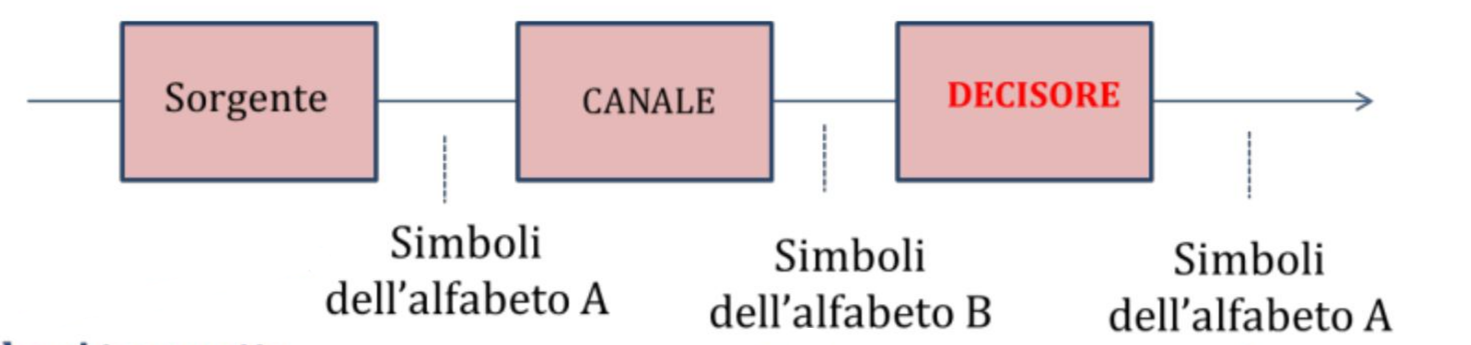
\includegraphics[scale=0.2]{img/decis.png}
\end{figure}
\defn{\textit{Regola di decisione:}} Dato un alfabeto in ingresso $A = \{a_1, \dots, a_r\}$ e uno di uscita $B = \{b_1, \dots, b_s\}$ una regola di decisione \`e una funzione $d:B \to A$ tale che 
\begin{equation}
    \forall b \in B \quad  \exists ! \hspace{4pt}  \hat{a} \in A : d(b) = \hat{a}
\end{equation}
\begin{mybox}{green}{\textbf{\textit{Esempio 7 : Regola di decisione per BSC}}}
Se si ha un BSC con matrice di canale
\begin{equation*}
    \mathcal{P} = \begin{bmatrix}
    0.9 & 0.1
    0.1 & 0.9
    \end{bmatrix}
\end{equation*}
si pu\`o decidere in due modi
\begin{equation*}
    \begin{cases}
    d(0) = 0 \land d(1) = 1 \\
    d(0) = 1 \land d(1) = 0
    \end{cases}
\end{equation*}
La prima regola di decisione non assicura l'assenza di errori ma, mediamente, sbaglier\`a solo nel 10\% dei casi. L'altra regola invece porta a una media del 90\% di errore.
\end{mybox}
In generale si ha che, per un canale con $r$ ingressi ed $s$ uscite, si possono avere $r^s$ regole di decisione. Ad ogni regola di decisione \`e associata un'incertezza ed il nostro obiettivo \`e determinare la migliore regola di decisione. La probabilit\`a di errore media $P_e$ \`e quindi associata ad una certa regola di decisione, in particolare, data una certa regola di decisione $d$, essa pu\`o essere scritta come
\begin{equation}
    P_e \coloneqq \sum_{b \in B} \underset{a \neq \hat{a}}{\sum_{a \in A}} p(a,b) = \sum_{b \in B} \underset{a \neq \hat{a}}{\sum_{a \in A}} p(b|a) p(a) = 1 - \underbrace{\sum_{b \in B} p(b|\hat{a})p (\hat{a})}_{=P_c}
\end{equation}
Dove $P_c$ indica la probabilit\`a di corretta decisione. Come si minimizza questa probabilit\`a? La regola di decisione ottima \`e data dal criterio di \textbf{massima verosimiglianza}:
\begin{align*}
    \min_{d(b)} P_e &= \min_{d(b)} 1 - P_c = \max_{d(b)} P_c = \max_{d(b)} \sum_{b \in B} p(b|\hat{a})p (\hat{a})\\
    &\text{ovvero } \min_{d(b)} p(b|\hat{a})p (\hat{a}), \quad \forall b \in B
\end{align*}
Il simbolo $\hat{a}$ viene quindi scelto come quello che massimizza la probabilità di aver ricevuto il simbolo $b$ condizionata alla trasmissione di $a$:
\begin{equation}
    d(b) = \hat{a} \iff p(b|\hat{a}) p(\hat{a}) \geq p(b|a) p(a), \hspace{10pt} \forall a\in A, b\in B
\end{equation}
che, nel caso di simboli equiprobabili\footnote{Se non si conosce la statistica della sorgente si applica il criterio ML considerando simboli equiprobabili. In questo caso si ottiene una regola di decisione sub-ottima.}, diventa
\begin{equation}
   d(b) = \hat{a} \iff p(b|\hat{a}) \geq p(b|a), \hspace{10pt} \forall a\in A, b\in B
\end{equation}
\subsection{Disuguaglianza di Fano}
Supponiamo, osservando una variabile aleatoria $B$, di voler stimare il valore assunto da un'altra variabile aleatoria $A$ correlata a $B$. La disuguaglianza di Fano connette la probabilit\`a di errore di indovinare il valore di $A$ con l'entropia condizionata $H(A|B)$. L'idea \`e che ci aspettiamo di poter stimare $A$ con una bassa probabilit\`a di errore solo se la probabilit\`a condizionata $H(A|B)$ \`e \textit{piccola}.

Indicando con $P_e$ la probabilit\`a di errore\footnote{In generale $P_e$ pu\`e essere dato da qualunque stimatore $g(B) = \hat{A}$: $P_e = Pr \{\hat{A} \neq A\}$.} si ha la che 
\begin{equation}
\label{eqn:fano}
    H(A|B) \leq H(P_e) + P_e\log (r-1)
\end{equation}
Il membro a destra \`e dato dalla somma di due contributi. Una volta osservato $B$ infatti:
\begin{itemize}
    \item Non si pu\`o determinare se il simbolo ricevuto è affetto da errore o no, e questo \`e il contributo dato da $H(P_e)$, quest'ultima infatti \`e la quantità di informazione di una sorgente binaria con simboli $\{errore, non$ $errore \}$, quindi la quantità di informazione necessaria all'osservatore per dire se c’è stato un errore.
    \item Se c’è errore, con probabilità $P_e$, non si pu\`o determinare quale dei restanti $r-1$ simboli si \`e sbagliato a stimare. Essendo una probabilit\`a condizionata si ha che il valore massimo che può assumere è quello di una sorgente senza condizionamento con $r-1$ simboli tutti equiprobabili, la cui incertezza \`e $\log (r-1)$ pesata per $P_e$. 
\end{itemize}
Ricordando che $r = |A|$ la disuguaglianza di Fano ci dice che l'entropia condizionata \`e massima per $P_e = 1 - \frac{1}{r}$ e vale $H(A|B) = \log r$. Questo avviene quindi quando la probabilit\`a di corretta decisione \`e uniforme sull'insieme $A$, ovvero quando $P_c = \frac{1}{r}$.

\begin{figure}[H]
    \centering
    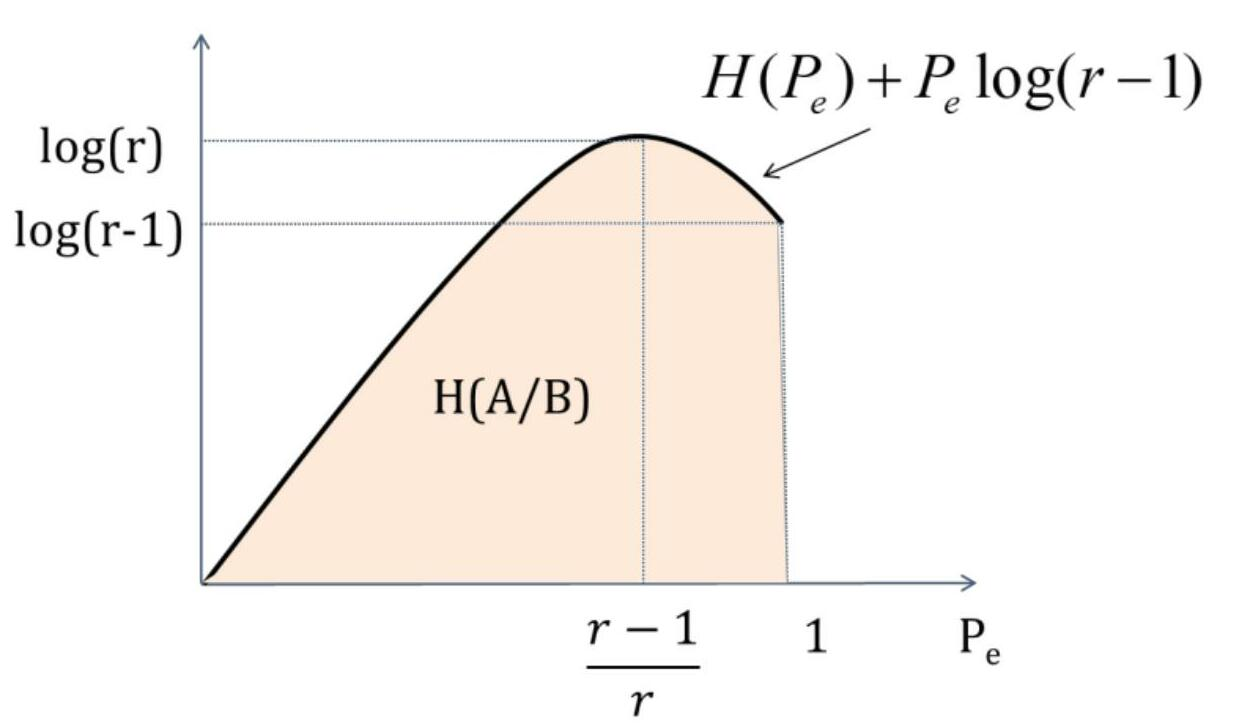
\includegraphics[scale=0.2]{img/fano.jpg}
    \caption{Rappresentazione grafica della disuguaglianza di Fano.}
\end{figure}
Si ha infatti che la funzione $H(P_e) + \log (r-1)$ \`e concava nell'intervallo $P_e \in [0, 1]$, quindi il massimo si ottiene in
\begin{align*}
    \frac{\partial}{\partial P_e} \Big \{ H(P_e) + P_e\log (r-1) \Big \} &= \frac{\partial}{\partial P_e} \Big \{ P_e \log \frac {1}{P_e} + (1-P_e) \log \frac{1}{1 - P_e} + P_e \log(r-1) \Big \} = \\
    &=\log \frac{1}{P_e} - \log \frac{1}{1-P_e} + \log (r-1) = \\
    &=\log \frac{(1-P_e)(r-1)}{P_e} = 0 \implies \frac{(1-P_e)(r-1)}{P_e} = 1 \\
    &\implies P_e = 1 - \frac{1}{r} = \frac{r-1}{r}
\end{align*}
\newline
Vediamo ora la dimostrazione della disuguaglianza di Fano data nella (\ref{eqn:fano}). Questa non \`e l'unica forma in cui si pu\`o presentare ma \`e la forma che pi\`u rapidamente ci permette di mostrare come questa fornisca un limite inferiore alla probabilità d'errore.
\begin{tcolorbox}[enhanced, breakable, frame hidden]
\textbf{Dim}: Proviamo che $H(A|B) - H(P_e) - P_e \log(r-1) \leq 0$. Scriviamo i due termini di entropia in funzione di $P_e$:
\begin{align*}
    H(P_e) + P_e \log (r-1) &= P_e \log \frac{1}{P_e} + P_c \log \frac{1}{P_c} + P_e \log (r-1) = P_e \log \frac{r-1}{P_e} + P_c \log \frac {1}{P_c} = \\
    &=\sum_{b \in B} \underset{a \neq \hat{a}}{\sum_{a \in A}} p(a,b) \log \frac{r-1}{P_e} + \sum_{b \in B} p(\hat{a},b) \log \frac{1}{P_c}
\end{align*}
\begin{align*}
    \hspace{-30pt}H(A|B) &= \sum_{a \in A} \sum_{b \in B} p(a,b) \info{a|b} = \underset{a \neq \hat{a}}{\sum_{a \in A}} \sum_{b \in B} p(a,b) \info{a|b} + \sum_{b \in B} p(\hat{a},b) \info{\hat{a}|b}
\end{align*}
da cui, facendo la differenza, si ha
\begin{align*}
&H(A|B) - H(P_e) + P_e \log (r-1) = \\
&= \underset{a \neq \hat{a}}{\sum_{a \in A}}\sum_{b\in B} p(a,b) \info{a|b} + \sum_{b \in B} p(\hat{a},b) \info{\hat{a}|b} - \sum_{b \in B} \underset{a \neq \hat{a}}{\sum_{a \in A}}  p(a,b) \log \frac{r-1}{P_e} - \sum_{b \in B} p(\hat{a},b) \log \frac{1}{P_c} \\
&=\underset{a \neq \hat{a}}{\sum_{a \in A}}\sum_{b\in B}  p(a,b) \log \frac{P_e}{p(a|b)(r-1)} + \sum_{b \in B} p(\hat{a},b) \log \frac{P_c}{p(\hat{a}|b)} = \\
&=\log e \Bigg [ \underset{a \neq \hat{a}}{\sum_{a \in A}}\sum_{b\in B}  p(a,b) \ln \frac{P_e}{p(a|b)(r-1)} + \sum_{b \in B} p(\hat{a},b) \ln \frac{P_c}{p(\hat{a}|b)} \Bigg ] \leq \\
&\leq \log e \Bigg [ \underset{a \neq \hat{a}}{\sum_{a \in A}}\sum_{b\in B}  p(a,b) \Big (\frac{P_e}{p(a|b)(r-1)} - 1 \Big ) + \sum_{b \in B} p(\hat{a},b) \Big ( \frac{P_c}{p(\hat{a}|b)} - 1 \Big ) \Bigg ] = \\
&=\log e \Bigg [ \underset{a \neq \hat{a}}{\sum_{a \in A}}\sum_{b\in B} \Big (   \frac{P_e p(b)}{r-1} - p(a,b) \Big ) + \sum_{b \in B} P_c p(b) - p(\hat{a},b) \Big ) \Bigg ] = \\
&=\log e \Bigg [ \underset{a \neq \hat{a}}{\sum_{a \in A}} \frac{P_e}{r-1} - p(a) + P_c - p(\hat{a}) \Bigg ] = \\
&=\log e \Bigg [ \frac{P_e(r-1)}{r-1} - \big (1 - p(\hat{a}) \big ) + P_c - p(\hat{a}) \Bigg ] = \\
&=\log e \Big [ P_e + P_c - 1\Big ] = 0 \\
&\hspace{400pt}\square
\end{align*}
\end{tcolorbox}

Si ha inoltre che la disuguaglianza vale come uguaglianza quando, $\forall b \in B$
\begin{equation*}
\begin{cases}
\frac{P_e}{p(a|b)(r-1)} = 1, & \forall a \in A \backslash \{\hat{a}\}\\
\frac{P_c}{p(\hat{a}|b)} = 1
\end{cases} \implies 
\begin{cases}
P_e = p(a|b) (r-1), & \forall a \in A \backslash \{\hat{a}\} \\
P_c = p(\hat{a}|b)
\end{cases}
\end{equation*}
ovvero quando, se si trasmette un simbolo $a$, si ha la stessa probabilità di sbagliare con uno qualsiasi degli altri simboli.

Se prendiamo la disuguaglianza di Fano e la relazione che lega informazione mutua ed equivocazione di canale si ha:
\begin{equation*}
    H(A|B) \leq H(P_e) + P_e \log (r-1) \land H(A|B) = H(A) - I(A;B) \geq H(A) - \mathcal{C}
\end{equation*}
da cui
\begin{equation}
    H(A) \leq H(A|B) \leq H(P_e) + P_e \log (r-1) + \mathcal{C}
\end{equation}

\begin{figure}[H]
    \centering
    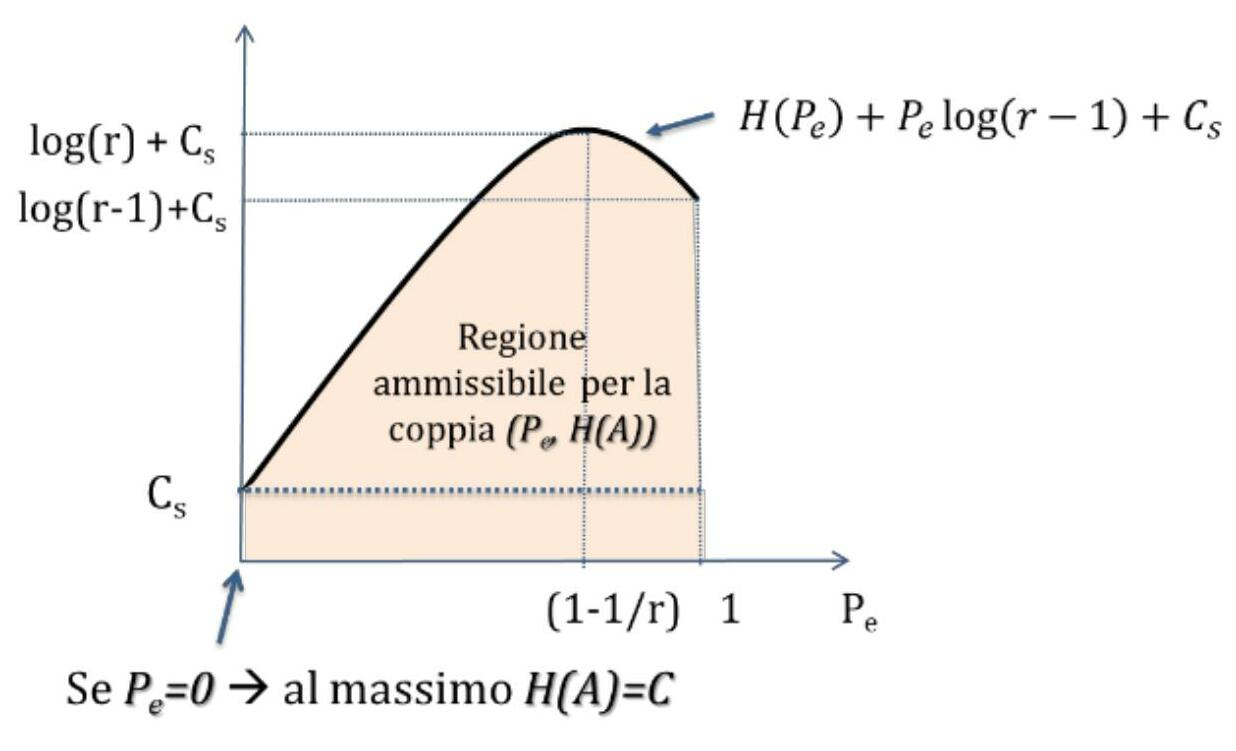
\includegraphics[scale=0.2]{img/equiv.jpg}
    \caption{Regione di di ammissibilit\`a per la coppia $\big ( P_e, H(A) \big )$.}
\end{figure}

Si ha quindi che \textit{se l’entropia della sorgente (il rate) supera la capacit\`a di canale \textbf{\`e impossibile trasmettere con probabilità di errore piccola a piacere}}. Se $H(A) - \mathcal{C} = \tau > 0$ si ha
\begin{equation*}
    H(P_e) + P_e \log (r-1) \geq \tau > 0
\end{equation*}
e quindi un limite inferiore per la $P_e$. Dal momento che esiste questo limite, dato un certo canale con capacità $\mathcal{C}$, vogliamo capire se c`è un modo per rendere la comunicazione più affidabile. \textbf{L’obiettivo è quindi quello di trovare un limite per la quantità di informazione che può essere trasmessa in modo affidabile su un canale rumoroso}. \\
L’affidabilità di una comunicazione può essere migliorata con la codifica di canale, il cui obiettivo consiste proprio nell’aumentare la resistenza dell’informazione al rumore presente sul canale. La codifica di canale \textit{trasforma} la sequenza di dati in ingresso al canale in una nuova sequenza intrinsecamente più robusta agli effetti del rumore. \textit{L’approccio adottato consiste solitamente nell’introdurre ridondanza}. Sfruttando tale ridondanza il decodificatore può ricostruire il messaggio originale anche in presenza di bit errati.
\begin{mybox}{green}{\textit{\textbf{Esempio 6} : \textbf{Codice a ripetizione}}}
Consideriamo un canale simmetrico binario con $p=0.01$ con simboli in ingresso equiprobabili.

\begin{minipage}{0.45\textwidth}
\begin{figure}[H]
    \centering
    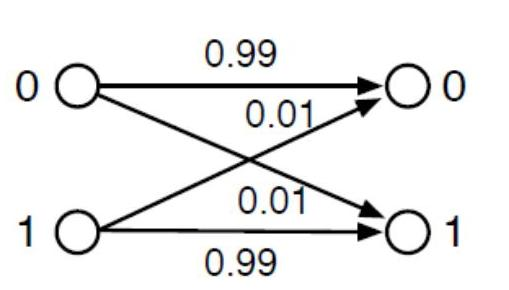
\includegraphics[scale=0.3]{img/bscese.jpg}
\end{figure}
\end{minipage}
\begin{minipage}{0.45\textwidth}
Si ha che 
\begin{equation*}
    \mathcal{P} = \begin{bmatrix}
    0.99 & 0.01 \\
    0.01 & 0.99 \\
    \end{bmatrix}
\end{equation*}
in cui la decisione ottima $d$ \`e data da
\begin{equation*}
    \begin{cases}
    d(0) = 0 \\
    d(1) = 1
    \end{cases} \implies P_e = \frac{0.01 + 0.01}{2} = 0.01
\end{equation*}
\end{minipage}

\vspace{10pt}
Proviamo a migliorare l’affidabilità con una semplice codifica di canale: il \textit{codice a ripetizione}, inviando il $bit$, ad esempio, 3 volte invece di una sola. In sostanza quindi si considera l’estensione di un BSC in cui i simboli che possono essere inviati sul canale sono solamente due $000, 1111$, mentre possono essere ricevute tutte le combinazioni di 3 bit (a seguito degli errori di trasmissione).
\end{mybox}
\begin{mybox}{green}{}
In ricezione la regola di decisione è abbastanza semplice: si sceglie $0$ se sono stati ricevuti più $0$ che $1$, mentre si sceglie $1$ nell'altro caso (avendo preso una ripetizione dispari non si ha mai ambiguità). Poiché la probabilità che $1$ bit venga trasmesso in maniera non corretta e uguale a $p=0.01$ per tutti i simboli, si ha dalla distribuzione binomiale
\begin{align*}
    P_e &= p^2(1-p) \left(
    \begin{array}{c}
      3 \\
      2
    \end{array}
  \right) + p^3(1-p)^0 \left(
    \begin{array}{c}
      3 \\
      3
    \end{array}
  \right) = \\
  &=3p^2(1-p) + p^3 = 3 \times 0.01^2 \times 0.99 + 0.01^3 \approx 3 \cdot 10^{-4}
\end{align*}
L'affidabilità è aumentata a costo di aumentare il numero di bit di ben 3 volte. Possiamo quindi dire che la velocità di trasmissione è ridotta di $1/3$. Se aumentiamo ancora il numero di bit vedremo sempre lo stesso andamento:

\begin{table}[H]
    \centering
    \begin{tabular}{ccc}
    $n$ & $P_e$ & $R$ \\
    \toprule
    $1$ & $10^{-2}$ & $1$ \\
    $3$ & $3$ $\cdot 10^{-4}$ & $1/3$ \\
    $5$ & $3\cdot 10^{-5}$ & $1/5$ \\
    $7$ & $4 \cdot 10^{-7}$ & $1/7$ \\
    $9$ & $10^{-8}$ & $1/8$ \\
    $\vdots$ & $\vdots$ & $\vdots$ \\
    \end{tabular}
    \label{tab:codic}
\end{table}
Quindi se nel tempo di $k$ simboli si trasmette un solo simbolo informativo la velocità di trasmissione si riduce di $k$ volte.
\end{mybox}

\subsection{Canale esteso}
\begin{figure}[H]
    \centering
    
\includegraphics[scale=0.2]{img/estchan.jpg}
\end{figure}
Nell'estensione del canale andiamo a considerare sorgenti estese $A^n, B^n$. Si ha che vale
\begin{align*}
    I(A^n;B^n) \leq n \mathcal{C}
\end{align*}
\begin{tcolorbox}[enhanced, breakable, frame hidden]
\textbf{Dim}:
\begin{align*}
    I(A^n;B^n) &= H(B^n) - H(B^n|A^n) = H(B^n) - \sum_{i=1}^n H(B_i|B_1, \dots, B_{i-1}, A^n) = \\
    &\overset{\eta}{=} H(B^n) - \sum_{i=1}^n H(B_i|A_i) \leq \sum_{i=1}^n H(B_i) - \sum_{i=1}^n H(B_i|A_i) = \sum_{i=1}^n I(A_i; B_i) \leq \\
    &\leq n \mathcal{C} \hspace{350pt} \square
\end{align*}
\end{tcolorbox}
Dove l'uguaglianza $\eta$ vale perche il canale \`e discreto e senza memoria, da cui $B_i$ dipdende unicamente da $A_i$ ed \`e quindi condizionalmente indipendente da tutto il resto. La prima disuguaglianza vale invece dalla (\ref{eqn:leq}) e la seconda dalla definizione di capactit\`a. \\
Si pu\`o estendere la disuguaglianza di Fano all'estensione $n$-esima del canale come
\begin{equation}
    H(A^n|B^n) \leq H(P_e^n) + P_e^n \log (r^n - 1)
\end{equation}
dove $P_e^n$ \`e la probabilit\`a di errore associata a una sequenza di $n$ simboli e \textcolor{red}{non} la potenza $n$-esima della $P_e$ per un simbolo.
Abbiamo visto che aumentando il numero di bit usati per codificare un simbolo della sorgente si riduce la $P_e$ ma anche la velocità con cui si trasmettono i dati. Consideriamo allora un altro esempio: dato lo stesso canale BSC visto sopra, cambiamo codifica, invece di inviare un bit per volta, ne inviamo due e codifichiamo il messaggio fatto da due bit in una parola di codice fatta da tre bit:
 
 \begin{minipage}{0.45\textwidth}
 \begin{figure}[H]
     \centering
     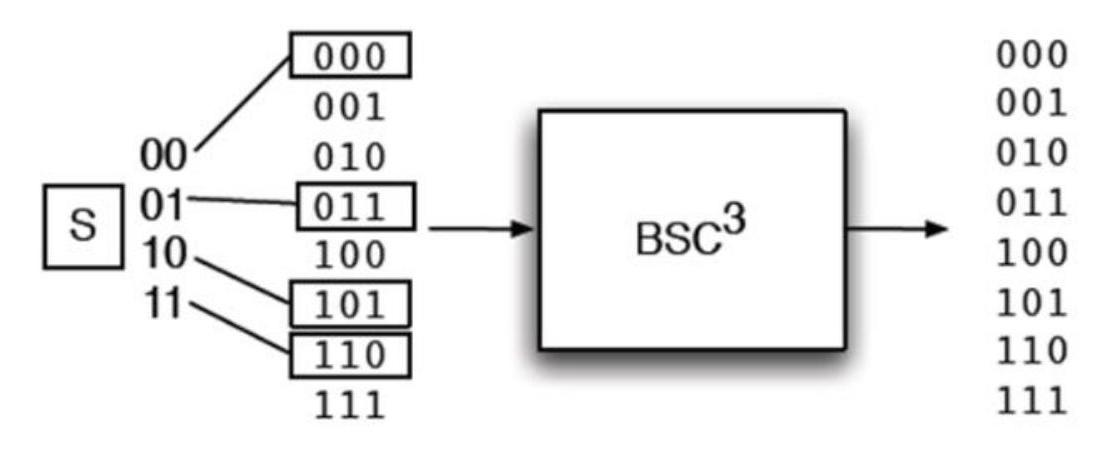
\includegraphics[scale=0.2]{img/bsc3.jpg}
 \end{figure}
 \end{minipage} \hfill
 \begin{minipage}{0.45\textwidth}
 La decisione ottima $d$ \`e data da
\begin{equation*}
    \begin{cases}
    d(000) = d(001) = 00 \\
    d(010) = d(011) = 01 \\
    d(100) = d(101) = 10 \\
    d(110) = d(111) = 11 \\
    \end{cases} \implies P_e \approx 2 \cdot 10^{-2}
\end{equation*}
Con un rate $R=\frac{2}{3}$ dal momento che vengono inviati $3$ bit per rappresentarne $2$.
\end{minipage}

La codifica di canale associa a blocchi di $k$ bit in ingresso blocchi di $n$ bit, con $n \geq k$ il che comporta che il \textbf{coding rate} $R_c$ segua la legge
\begin{equation}
    R_c \coloneqq \frac{k}{n}
\end{equation}
dal momento che, se per ogni parola della sorgente lunga $k$ bit se ne inviano $n$ la velocità di trasmissione si ridurr\`a: se invio $1$ $bit$ ogni $T$ unit\`a di tempo (ad esempio secondi): senza codifica sono necessari $kT$ unit\`a di tempo per terminare la comunicazione, con la codifica sono necessari $nT$ unit\`a di tempo, con $n\geq k$. Abbiamo quindi una struttura di questo tipo:
\begin{figure}[H]
    \centering
    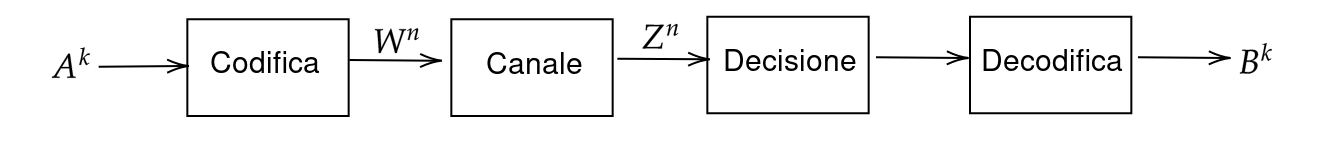
\includegraphics[scale=0.3]{img/diagramma.png}
\end{figure}
In cui, seguendo l'esempio con $k=2, n=3$, potremmo avere $A^2 = \{00, 01, 10, 11\}, W^3 = \{000, 011, 101, 110\}$ e $Z^3 = \{000, 001, 010, 011, 100, 101, 110, 100\}$. In questo sistema si ha che
\begin{itemize}
    \item $H(A^k|B^k) = H(A^k) - I(A^k;B^k)$
    \item Con i canali in cascata: $I(A^k; B^k) \leq I(W^n;Z^n)$
    \item Con un canale esteso: $I(W^n;Z^n) \leq n \mathcal{C}$
\end{itemize}
Questo comporta
\begin{equation*}
    \begin{cases}
    H(A^k|B^k) \geq H(A^k) - n \mathcal{C} = kH(A) - n \mathcal{C} \\
    H(A^k|B^k) \leq H(P_e^n) + P_e^n \log (r^k - 1)
    \end{cases} \implies k H(A) \leq H(P_e^n) + P_e^n \log (r^k -1) + n \mathcal{C}
\end{equation*}
Nel limite in cui $P_e \to 0$ si ha che 
\begin{equation*}
    kH(A) \leq n \mathcal{C} \implies H(A) \leq \frac{n}{k} \mathcal{C} = \frac{\mathcal{C}}{R_c}
\end{equation*}

\begin{minipage}{0.4\textwidth}
quindi deve essere che 
\vspace{15pt}
\begin{mybox}{blue}{}
\vspace{-10pt}
\begin{equation}
    R = R_c H(A) \leq \mathcal{C}
\end{equation}
\end{mybox}
\end{minipage} \hfill
\begin{minipage}{0.4\textwidth}
\begin{figure}[H]
    \centering
    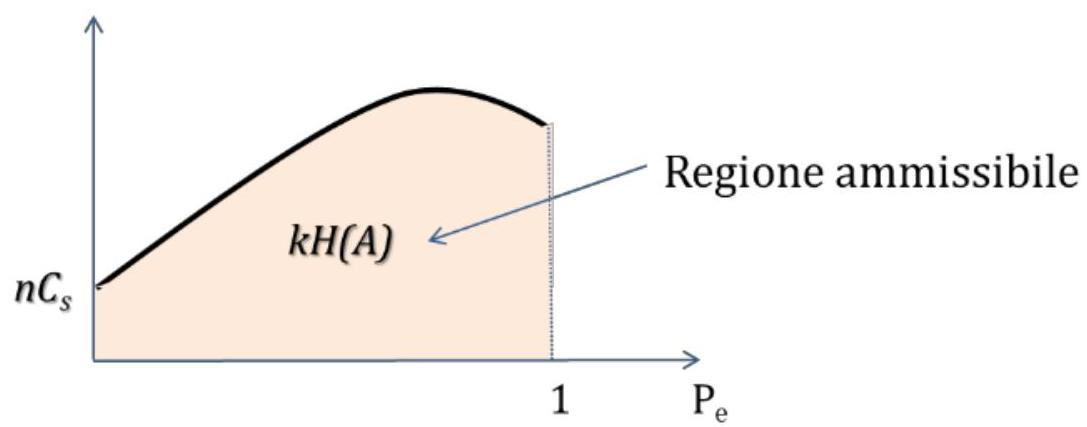
\includegraphics[scale=0.2]{img/ammiss.jpg}
\end{figure}
\end{minipage}

ovvero che, per poter lavorare nella regione $P_e \rightarrow 0$ si deve:
\begin{itemize}
    \item \textbf{Ridurre il rate di trasmissione}:
    \begin{enumerate}
        \item \textit{Riducendo il rate} (entropia) \textit{della sorgente} $A$, quindi comprimendo di pi\`u (non \`e detto che sia possibile).
        \item Ridcuendo $R_c$, ovvero \textit{aumentando la ridondanza della codifica di canale}: fissata $H(A)$ se la sorgente emette un bit ogni $T_s$ unit\`a di tempo, con modulazione binaria la banda necessaria $B$ sarebbe, se $R_c = 1$
        \begin{equation*}
            B \approx \frac{1}{T_s}
        \end{equation*}
        se invece il canale deve far passare $n$ bit in $kT_s$ unit\`a di tempo la banda necessaria sarebbe
        \begin{equation*}
            B \approx \frac{n}{kT_s} = \frac{R_c}{T_s}
        \end{equation*}
        il che implica che \textit{serve una banda maggiore}.
    \end{enumerate}
    \item \textbf{Aumentare la capacità di canale} $\mathcal{C}$ aumentando il \textit{Rapporto Segnale Rumore} sul canale: la $P_e$ si ridurr\`a dal momento che il canale introduce una minore equivocazione.
\end{itemize}
\subsection{Secondo Teorema di Shannon}
Il secondo teorema di Shannon da un’altra possibilità, ci dice che fissato il rate di sorgente e la capacità di canale, si può mantenere costante il rapporto $R_c = \frac{n}{k}$ (ovvero non aumentando la banda) \textbf{incrementando la lunghezza del blocco in ingresso al codificatore}. In sostanza dimostra che \textit{è possibile ridurre arbitrariamente la probabilità di errore, con il vincolo che il rate di trasmissione sia inferiore alla capacita di canale}.

Supponiamo di avere una sorgente discreta senza memoria con alfabeto $A$, entropia $H(A)$ e un canale discreto senza memoria con capacità per simbolo pari a $\mathcal{C}$ $[bit/simbolo]$. Il \textbf{Secondo Teorema di Shannon} afferma che

\textit{Esiste un sistema di codifica con $R_c = \frac{k}{n}$ e $R = R_c H(A) < \mathcal{C}$ che permette la trasmissione dell’informazione emessa dalla sorgente sul canale con una probabilità di errore arbitrariamente piccola.}

Questo pu\`o essere espresso come
\begin{equation}
    \forall \epsilon > 0, \exists n_0 \in \mathbb{N}: \forall n > n_0 \text{ si ha } P_e < \epsilon 
\end{equation}
ed in particolare si pu\`o scrivere, detta $E(\cdot)$ una funzione  convessa decrescente e positiva in $[0,\mathcal{C}]$
\begin{equation}
    P_e < e^{-nE(R_s)} \text{ con }R_s \coloneqq R_c H(A)
\end{equation}

Il Secondo Teorema di Shannon \textit{non fornisce dettagli sul sistema di codifica necessario} per ottenere probabilità d’errore arbitrariamente piccola, ma afferma solo che, \textit{se} $R < \mathcal{C}$, esso \textit{\textbf{esiste}}. Nella pratica, si può verificare che per ridurre la probabilità d’errore si deve incrementare il numero di $bit$ in ingresso al codificatore. Per $n \to \infty$ per\`o il tempo necessario per la trasmissione del messaggio codificato tende all’infinito e la complessità di codifica e decodifica cresce.
\subsection{Canale Gaussiano}
Fino ad ora abbiamo considerato canali discreti. Nella realtà le informazioni vengono inviate in canali analogici e si devono quindi considerare sorgenti analogiche. Studiamo in particolare il canale con rumore bianco gaussiano (\textit{AWGN})\footnote{Questo canale \`e un buon modello per molte comunicazioni, come quella telefonica o quella satellitare.}, che è caratterizzato da un modello a rumore additivo tra ingresso $X$ ed uscita $Y$:
\begin{equation}
    Y = X + Z
\end{equation}
in cui il rumore $Z = \mathcal{N}(0; \sigma_z^2)$ con $X \perp Z$ ($X$ e $Z$ incorrelate). \textit{Data la bianchezza del rumore il canale \`e quindi senza memoria e stazionario}. \\
Anche nel caso di segnali analogici poi vale quanto abbiamo visto, e la capacità è definita come il massimo
dell’informazione mutua:
\begin{align*}
    \mathcal{C} &= \max_{X} I(X;Y) = \max_{X} \big [ h(Y) - h(Y|X) \big ]= \\
    &=\max_{X} \big [ h(Y) - h(X+Z|X) \big ]= \max_{X} \big [ h(Y) - h(Z|X) \big ]= \\
    &=\max_{X} \big [ h(Y) - h(Z) \big ] = \max_{X} \big [ h(Y) - \frac{1}{2}\log (2 \pi \sigma_z^2 e )\big ]
\end{align*}
che si ottiene quando $Y$ \`e gaussiana
\begin{equation*}
    \mathcal{C} = \frac{1}{2}\log (2 \pi \sigma_y^2 e) - \frac{1}{2}\log (2 \pi \sigma_z^2 e) = \frac{1}{2} \log \frac{\sigma_y^2}{\sigma_z^2}
\end{equation*}
ed essendo $X \perp Z$ si ha $\sigma_y^2 = \sigma_x^2 + \sigma_z^2$ da cui
\begin{equation}
    \mathcal{C} = \frac{1}{2} \log \bigg ( 1 + \frac{\sigma_x^2}{\sigma_z^2} \bigg )
\end{equation}

Stiamo per\`o considerando un canale con banda infinita: nella pratica tutti i canali hanno banda limitata $[-B,B]$ e, se non vogliamo avere aliasing, il segnale deve essere campionato\footnote{Per il Teorema del Campionamento di Nyquist-Shannon.} con una frequenza almeno pari a $2B$ campioni$/s$. Ogni campione di segnale ha potenza $P_X = \sigma_x^2$ mentre la potenza del rumore, assumento che la densità spettrale di potenza del segnale sia $\sigma_x^2 = \frac{N_0}{2} \frac{[W]}{[Hz]}$, \`e data da $P_Z = \sigma_z^2 = N_0 B$ da cui
\begin{equation*}
    \mathcal{C} = \frac{1}{2} \log \bigg ( 1 + \frac{\sigma_x^2}{N_0 B} \bigg ) \hspace{10pt} \frac{bit}{\text{trasmissione}}
\end{equation*}
e se teniamo in considerazione la frequenza di campionamento $f = 2B$ possiamo usare il canale $2B$ volte al secondo, quindi
\begin{equation}
    \mathcal{C} = f \frac{1}{2} \log \bigg ( 1 + \frac{\sigma_x^2}{N_0 B} \bigg ) = B \log \bigg ( 1 + \frac{\sigma_x^2}{N_0 B} \bigg ) = B \log \big (1 + SNR \big ) \hspace{5pt} \frac{bit}{s}
\end{equation}
che è famosa formula di Shannon della capacità di un canale \textit{AWGN}. \\
Dalla formula si vede che la capacità dipende dalla banda e dal \textit{SNR}, quindi dalla potenza del segnale in ingresso $P_x$. Aumentando la potenza di trasmissione aumenta il \textit{SNR} e ovviamente aumenta la capacità, ma la crescita è logaritmica. Aumentando la banda $B$ aumenta il termine a moltiplicare ma anche la quantità di rumore che entra nel segnale, quindi si ha un asintoto
\begin{align*}
    \lim_{B \to \infty} \mathcal{C} &= \lim_{B \to \infty} B \log \bigg ( 1 + \frac{\sigma_x^2}{BN_0} \bigg ) = \\
    &=\lim_{B \to \infty} (\log e) B \ln \bigg ( 1 + \frac{\sigma_x^2}{BN_0} \bigg ) \approx \lim_{B \to \infty} (\log e) B \frac{\sigma_x^2}{BN_0} = (\log e) \frac{\sigma_x^2}{N_0}
\end{align*}
dove si \`e usato l’approssimazione al primo ordine $\ln (1 + x) \approx x$ con $x \ll 1$. \`E chiaro quindi che, anche aumentando la banda $B$ non si pu\`o scendere sotto il limite di $\approx 1.44 \sigma_x^2/N_0$.

\subsection{Curva di Shannon}
Introduciamo adesso la curva di Shannon, che mostra l'esistenza di un \textit{trade-off} tra potenza del segnale in ingresso $P_x$ e banda $B$ in ogni sistema di comunicazione. Dal momento che deve essere $R < \mathcal{C}$ si deve avere
\begin{equation}
    R < B \log \bigg ( 1 + \frac{P_x}{N_0 B}\bigg )
\end{equation}
dividendo entrambi i membri per $B$ si ottiene l'\textit{efficienza spettrale} $r \coloneqq R/B$
\begin{equation}
    r < \log \bigg ( 1 + \frac{P_x}{N_0 B} \bigg )
\end{equation}
ovvero il numero di $bits$ per secondo che possono essere trasmessi in un'unit\`a di banda (in 1 $Hz$). Osservando che $P_x = E_b R$, dove $E_b$ \`e l'energia per bit trasmesso, otteniamo
\begin{equation}
\label{eqn:shanncurve}
    r < \log \bigg (1 + r \frac{E_b}{N_0} \bigg )
\end{equation}
Questa relazione definisce le regioni di ammissibilit\`a di efficienza spettrale al variare del rapporto $E_b/N_0$. Il luogo dei punti in cui $r = \log (1 + r E_b/N_0 )$ prende il nome di \textbf{curva di Shannon} (vedi Figura \ref{fig:shcrv}). Quest'ultima divide il piano $(E_b/N_0, r)$ in due parti: la regione sotto la curva (in blu) rappresenta l'insieme dei punti per cui \`e possibile ottenere una comunicazione affidabile (quella sopra in cui non \`e possibile). Per studiare il comportamento del $ENR$ (\textit{Energy-Noise Ratio}) al variare di $r$ eleviamo alla potenza di $2$ entrambi i membri della \ref{eqn:shanncurve}, da cui
\begin{equation}
\frac{2^r - 1}{r} < \frac{E_b}{N_0}
\end{equation}
Possiamo quindi studiare il comportamento asintotico:
    \begin{equation*}
    \begin{cases}
        r \to \infty \implies \frac{E_b}{N_0} \to \infty \\
        r \to 0 \implies \frac{E_b}{N_0} \to \ln 2
    \end{cases}
    \end{equation*}
ovvero che la curva di Shannon ha un asintoto verticale in $E_b/N_0 = \ln 2 \approx 1.6$ $dB$ al di sotto del quale non \`e possibile avere una trasmissione affidabile, per ogni valore di $r$.
\begin{figure}[H]
    \centering
    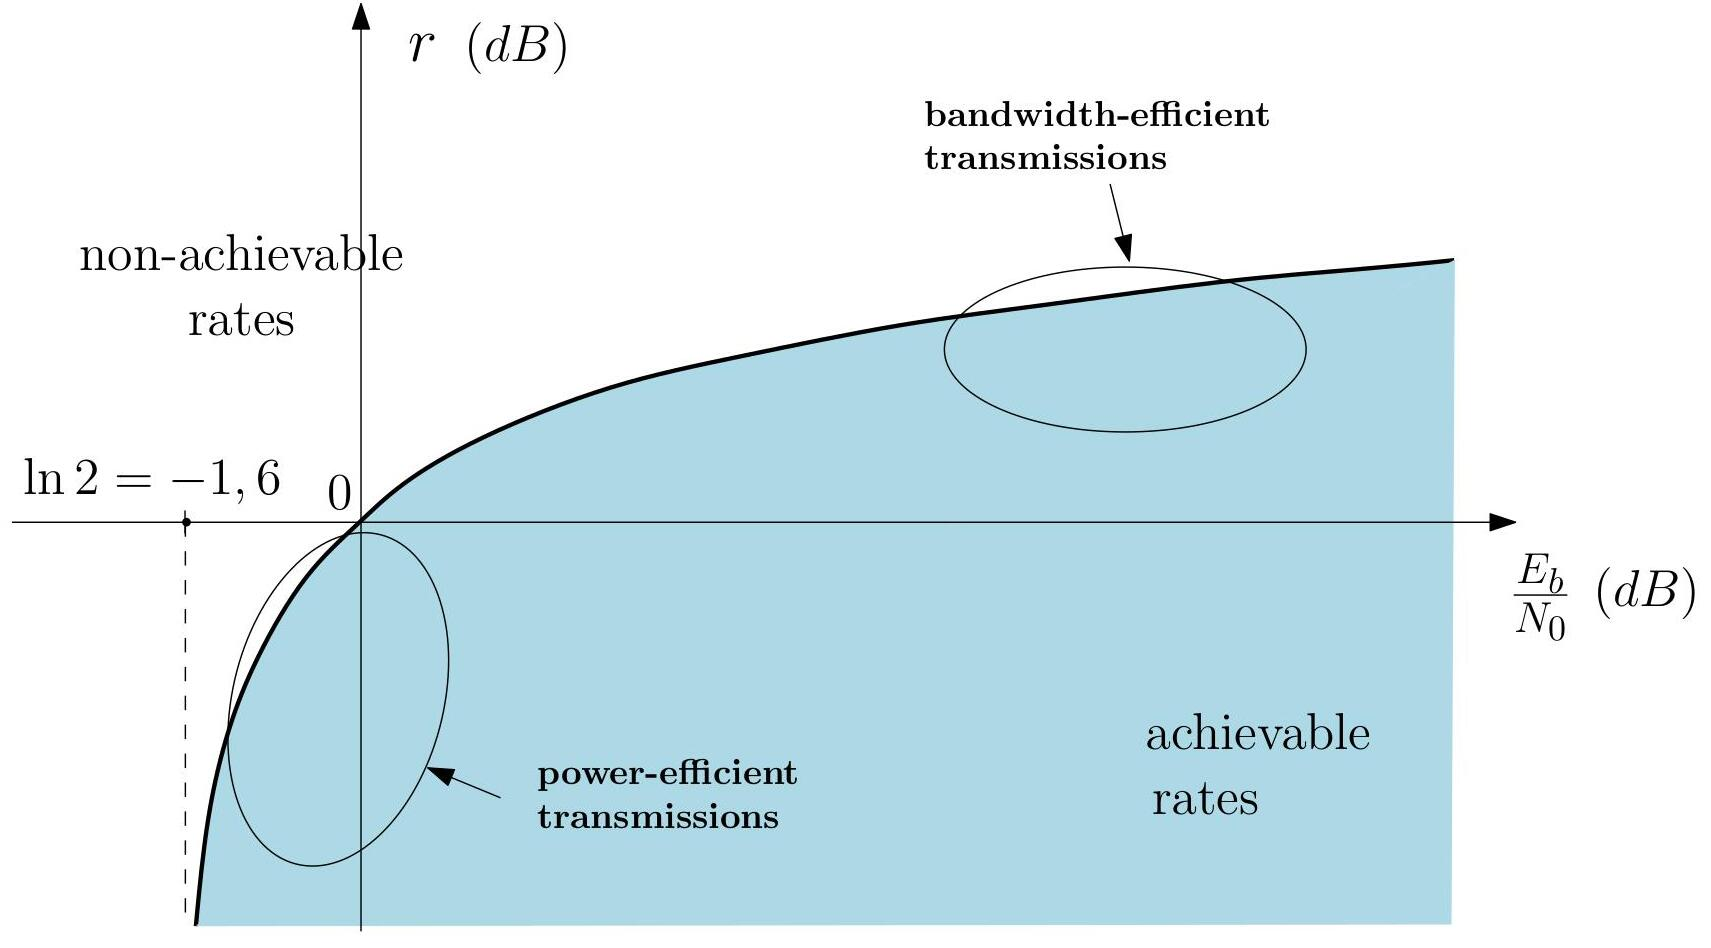
\includegraphics[scale=0.2]{img/shanno.jpg}
    \caption{Curva di capacit\`a di Shannon.}
    \label{fig:shcrv}
\end{figure}
La curva che si ottiene è teorica, ma tali risultati sono molto utili nella progettazione di un sistema reale, in quanto definiscono il \textit{\textbf{limite superiore} delle prestazioni ottenibili da un sistema} modellabile con un canale corrotto da rumore \textit{AWGN}. Nella regione dei punti operativi (raggiungibili) ovviamente più il punto di lavoro reale che si riesce ad ottenere si avvicina alla curva limite $(R=C)$ più il sistema è efficiente. Per le comunicazioni il cui principale limite è la potenza di trasmissione ($r \ll 1$) si hanno trasmissioni efficienti in potenza, mentre per i sistemi dove è la banda ad essere il limite principale ($r \gg 1$) si hanno trasmissioni efficienti in banda.

\newpage
\begin{appendices}
\section{Richiami (TODO)}
\subsection{Richiami di probabilit\`a}
\label{sec:prob}

\subsection{Richiami sui processi stocastici}
\label{sec:stoc}

\subsection{Notazione}
Alcuni apici che useremo nel corso di questi appunti, che verranno inseriti ogni qual volta si debba esplicitare il motivo del passaggio matematico in cui sono stati invocati:

\begin{align*}
    &\alpha : \sum_{x} p(x) = 1 \\
    &\beta : \ln x \leq x - 1 \text{ con } \ln x = x - 1 \iff x = 1 \\
    &\gamma : p(a,b) = p(a|b)p(b) \\
    &\delta : \sum_{y} p(x,y) = p(x)
\end{align*}
\end{appendices}

\end{document}

